%%
%	version 2.0, 2017, Authors : Filipe Marques; (original Master Degree Thesis Template authors:) Miguel Amador and João Marques.
%%
\documentclass[defaultstyle,12pt,master,Helvetica]{01.thesis}
%Use 01.thesis_pt instead for PT version 
%Dummy text if written by default in English. Just changed to whatever you need.
% Helvetica is a similar font to Arial, with small differences.

%% Packages
\typeout{}
\typeout{--------------------------------------------------------------}
\typeout{ +---+ Thesis Template                            }
\typeout{ +---+      Version 2.0, November 2017                         }
\typeout{ +---+  for Instituto Superior Tecnico (IST),                 }
\typeout{ +---+  Universidade Técnica de Lisboa                         }
\typeout{ * Using Thesis Style from Pedro Tomás                                }
\typeout{ * Created to write Dissertations                             }
\typeout{ * Conforms with IST Doctoral Degree format and with most important packages setup        }
%\typeout{ * Should conform with IST PhD Degree format (not verified)   }
\typeout{                                                              }
\typeout{ AUTHOR: Filipe Marques; (original Master Degree Thesis Template authors:) Miguel Amador and João Marques                                          }
\typeout{                                                              }
\typeout{Important: Use all files in the archive, since this is based in all them. Modify dummy files at wish.                                                              }
\typeout{--------------------------------------------------------------}
\typeout{}

% Defines an additional alphabet... not required in most cases
% ------------------------------------------------------------
% \DeclareMathAlphabet{\mathpzc}{OT1}{pzc}{m}{it}

% PACKAGE babel:
% ---------------
% The 'babel' package may correct some hyphenisation issues of latex. 
% However in most situations it is not required.
\usepackage[english,portuguese]{babel}


% PACKAGE fontenc:
% -----------------
% chooses T1-fonts and allows correct automatic hyphenation.
%\usepackage[T1]{fontenc}
%\usepackage[latin1]{inputenc}
\usepackage[utf8]{inputenc}
\usepackage[T1]{fontenc}
%\usepackage{lmodern} %will change font type

% Package ulem.
\usepackage{ulem} % Allows the use of other text emphatizer commands
\normalem %defines \emph{} to italic, instead of underline. 
\raggedbottom %declaration makes all pages the height of the text on that page. No extra vertical space is added. The \flushbottom declaration makes all text pages the same height, adding extra vertical space when necessary to fill out the page.

% PACKAGE date time:
% -----------------
% Lets you alter the format of the date that \today returns.
\usepackage{datetime}
\newdateformat{todaythesis}{%
  \monthname[\THEMONTH]  \THEYEAR}

% PACKAGE latexsym:
% -----------------
% Defines additional latex symbols. May be required for thesis with many math symbols.
\usepackage{latexsym}

% MATH PACKAGES amsthm, amssymb, amsfonts...:
% -------------------------------------------
% This package is typically required. Among many other things it adds the possibility
% to put symbols in bold by using \boldsymbol (not \mathbf); defines additional 
% fonts and symbols; adds the \eqref command for citing equations. I prefer the style
% "(x.xx)" for referering to an equation than to use "equation x.xx".
\usepackage{amsthm, amssymb, amsfonts, amsbsy}
\usepackage{mathtools}%The mathtools package fixes some amsmath quirks and adds some useful settings, symbols, and environments to amsmath.
\usepackage[dvipsnames]{xcolor}
\usepackage{cancel} % xcolor to change the texto color; cancel to use a cancel line in equations.
%https://en.wikibooks.org/wiki/LaTeX/Colors

% PACKAGE TABLES multirow, colortbl, longtable:
% ---------------------------------------
% These packages are most usefull for advanced tables. The first allows to join rows 
% throuhg the command \multirow which works similarly with the command \multicolumn
% The second package allows to color the table (both foreground and background)
% The third package is only required when tables extend beyond the length of one page;
% with compatibilities with the tabular environment. The last allow the definitions of landscape pages, allowing the use of a different orientation for wider graphics or tables. See package documentation to see the implementation.
\usepackage{multirow}
\usepackage{colortbl}
\usepackage{supertabular}
\usepackage{pdflscape}
% \usepackage{longtable}
\usepackage{tabularx}	% (default: necessary for the cover)
\usepackage{longtable,tabu}

% PACKAGE GRAPHICS graphics, epsfig, caption, etc...:
% ---------------------------------------------
% Packages for figures... well you will certainly need these packages, with the exception
% of the 'caption' package. This only allows to define extra caption options.
% Notice that subfigure allows to place figures within figures with its own caption. It
% should be avoided to create an eps file with subfigures. That will mean that you won't be 
% able to reference those subfigures. Instead create an EPS file (the only graphics format supported
% by latex) for each of the subfigures and then use the command \subfigure (see below).
\usepackage{graphics}
\usepackage{graphicx}
%\usepackage[pdftex]{graphicx} %> esta selecção provoca colisão com epsfig e caption...
\usepackage{epsfig}	%colisao com graphicx
\usepackage[font=small,labelfont=bf,textfont=normalfont]{caption}
\usepackage{caption} 	%to alter captions  (\usepackage[footnotesize,bf,center]{caption})
%\usepackage[hang,small,bf]{subfigure} %deprecated > use subfig or subcaption:
\usepackage{subcaption}	%for subfigures
\usepackage{dcolumn}
\usepackage{bm}
\usepackage{booktabs}
\usepackage{rotating}

\usepackage{color}% to alter text colour
\usepackage{pstricks} % to inkscape latex... not working
\usepackage{import} %to pdf-tex import from different place

% PACKAGE algorithmic, algorithm
% ------------------------------
% These packages are required if you need to describe an algorithm.
% \usepackage{algorithmic}
% \usepackage[chapter]{algorithm}

% PACKAGE natbib/cite/biblatex
% -------------------
% The three packages are not compatible, and you should use one of the two. Notice however that the
% IEEE BiBTeX stylesheet is imcompatible with the natbib package. If using the IEEE format, use the 
% cite package instead
%% Natbib
%\usepackage[square,numbers,sort&compress]{natbib}
\usepackage{natbib}
%% Cite
%\usepackage{cite}
%% Biblatex (Not working)
%\usepackage{csquotes}
%\usepackage[backend=biber,style=authoryear]{biblatex}


% PACKAGE acronyum
% -----------------
% This package is most useful for acronyms. The package guarantees that all acronyms definitions are 
% given at the first usage. IMPORTANT: do not use acronyms in titles/captions; otherwise the definition 
% will appear on the table of contents.
\usepackage[printonlyused]{acronym}
\usepackage[titletoc,title,header]{appendix}
\usepackage[noauto]{chappg}
%The following line assures that each chapter deals with acronyms idependently.
%You may also do it manually by calling acresetall anywhere in the documento to reset the acronyms behaviour. 
\preto\chapter\acresetall

% PACKAGE extra_functions VER COMO DEVE SER
% -----------------
% My Personal package: defines the following commands:
% \fancychapter{chaptername) -> Prints a fancier chapter (you can also use the fancychapter package for this)
% \hline{width} -> use for a replacement of the \hline command
% \Mark1, \Mark2, \Mark3, ...
\usepackage{00.extra_functions}

\usepackage{xr-hyper}

% PACKAGE hyperref
% -----------------
% Set links for references and citations in document
% Some MiKTeX distributions have faulty PDF creators in which case this package will not work correctly
% Long live Linux :D
\usepackage[hidelinks,plainpages=false]{hyperref}
\hypersetup{
  colorlinks=false,
  citecolor=red,
  breaklinks=true,
  bookmarksnumbered=true,
  bookmarksopen=true,
  pdftitle={Thesis Title},
  pdfauthor={Author Name},
  pdfsubject={Doctoral Thesis in Electrical and Computer Engineering},
  pdfcreator={Document Creator Name},
  pdfkeywords={Thesis}}
%\usepackage[pdftex,bookmarks,colorlinks,breaklinks]{hyperref}  % PDF hyperlinks, with coloured links
%%\hypersetup{linkcolor=blue}
%\hypersetup{linkcolor=black}
\usepackage{float}
%\usepackage[final]{00.listofsymbols}
\usepackage{00.symlist}

% Set paragraph counter to alphanumeric mode
% \renewcommand{\theparagraph}{\Alph{paragraph}~--}
\renewcommand{\theparagraph}{}

\usepackage{enumitem}	% para set list
\usepackage{algpseudocode} % algorithmic pseudocode
\usepackage[chapter]{algorithm}

\usepackage{scrextend}
% \usepackage{marginnote}%temporary notes at the margin
\usepackage{multicol} %multiple columns environment
%solves figure problem: http://tex.stackexchange.com/questions/12262/multicol-and-figures
\newenvironment{Figure}
{\par\medskip\noindent\minipage{\linewidth}}
{\endminipage\par\medskip}

\usepackage{siunitx}
\sisetup{load-configurations = abbreviations}
%%% -------------------- declares extra units
\DeclareSIUnit\Mtoe{\mega \tonne oe} % use: \SI{100}{\Mtoe}
\DeclareSIUnit\GWh{GWh} % use: \SI{100}{\GWh}  (not \GW\hour = GW h )
%%% -------------------------------------------------

\usepackage{wrapfig} % to wrap text around small figures
\usepackage{dcolumn} %dcolumns in tables : https://en.wikibooks.org/wiki/LaTeX/Tables#Defining_multiple_columns

\usepackage{makeidx} %necessary?

%%%%%%%%%%%%

\usepackage{times}
\usepackage{etoolbox}
\usepackage{inconsolata}
\usepackage{nicefrac}
\usepackage{empheq}
\usepackage{url}
\usepackage{xspace}
\usepackage{enumitem}
\usepackage{stmaryrd}
\usepackage{tikz}
\usetikzlibrary{bayesnet}

% Gantt charts
\usepackage{pgfgantt}

\usepackage{stmaryrd}
\SetSymbolFont{stmry}{bold}{U}{stmry}{m}{n}

\usepackage{lscape}
%% Page formatting
\hoffset 0in
\voffset 0in

%Alternative set of page geometry
%\oddsidemargin 0.71cm
%\evensidemargin 0.04cm
%\marginparsep 0in
%\topmargin -0.25cm
%\textwidth 15cm
%\textheight 23.5cm

\usepackage[top=2.5cm, bottom=2.5cm, inner=4.0cm, outer=2.9cm]{geometry}

\usepackage{fancyhdr}
\pagestyle{fancy}
\renewcommand{\chaptermark}[1]{\markboth{\thechapter.\ #1}{}}
\renewcommand{\sectionmark}[1]{\markright{\thesection\ #1}}
\fancyhf{}
%\fancyhead[LE]{\bfseries\nouppercase{\leftmark}}
%\fancyhead[RO]{\bfseries\nouppercase{\rightmark}}
\fancyfoot[LE,RO]{\bfseries\small\thepage}
\renewcommand{\headrulewidth}{0.0pt}
\renewcommand{\footrulewidth}{0.0pt}
\addtolength{\headheight}{2pt} % make space for the rule
\fancypagestyle{plain}{% Used in Chapter titles
	\fancyhead{} % get rid of headers
	\renewcommand{\headrulewidth}{0pt} % and the line
	\renewcommand{\footrulewidth}{0pt}
	\fancyfoot[LE,RO]{\bfseries\small\thepage}
}

\fancypagestyle{begin}{%
	\fancyhead{}
	\renewcommand{\headrulewidth}{0pt}
	\renewcommand{\footrulewidth}{0pt}
	\fancyfoot[LE,RO]{\bfseries\small\thepage}
}
\fancypagestyle{document}{%
	\fancyhf{}
	\fancyhead[LE]{\bfseries\nouppercase{\leftmark}}
	\fancyhead[RO]{\bfseries\nouppercase{\rightmark}}
	\fancyfoot[LE,RO]{\bfseries\small\thepage}
	%\renewcommand{\headrulewidth}{0pt}
	%\renewcommand{\footrulewidth}{0pt}
	\addtolength{\headheight}{2pt} % make space for the rule
}
\fancypagestyle{documentsimple}{%
	\fancyhf{}
	\fancyfoot[LE,RO]{\bfseries\small\thepage}
	%\renewcommand{\headrulewidth}{0pt}
	%\renewcommand{\footrulewidth}{0pt}
	\addtolength{\headheight}{2pt} % make space for the rule
}
\setcounter{secnumdepth} {5}
\setcounter{tocdepth} {2}
\renewcommand{\thesubsubsection}{\thesubsection.\Alph{subsubsection}}

% Removed deprecated package subfigure. See if relevant if you choose to use the subfig package instead.
%\renewcommand{\subfigtopskip}{0.3 cm}
%\renewcommand{\subfigbottomskip}{0.2 cm}
%\renewcommand{\subfigcapskip}{0.3 cm}
%\renewcommand{\subfigcapmargin}{0.2 cm}

\graphicspath{{Figures/}}

\setlength{\parskip}{0.5em}
%% Custom commands
\newcommand{\smap}{SparseMAP\xspace}
\newcommand*{\wrt}{\textit{w.\hspace{.07em}r\hspace{.07em}.t.}\@\xspace}
\newcommand*{\eg}{\textit{e.\hspace{.07em}g.}\@\xspace}
\newcommand*{\ie}{\textit{i.\hspace{.07em}e.}\@\xspace}
\newcommand*{\cf}{\textit{cf.}\@\xspace}
\newcommand*{\lhs}{\textit{l.\hspace{.07em}h\hspace{.07em}.s.}\@\xspace}
\newcommand*{\rhs}{\textit{r.\hspace{.07em}h\hspace{.07em}.s.}\@\xspace}
\newcommand{\eqnref}[1]{Equation~\ref{#1}}
\newcommand{\chapref}[1]{Chapter~\ref{#1}}
\newcommand{\secref}[1]{\S\ref{#1}}
\newcommand{\figref}[1]{Figure~\ref{#1}}
\newcommand{\tableref}[1]{Table~\ref{#1}}
\newcommand{\appref}[1]{Appendix~\ref{#1}}

% font for small caps
% \newcommand*{\fonttextsc}{\fontfamily{lmtt}\selectfont}

\let\log\relax
\let\exp\relax
\let\min\relax
\let\max\relax
\DeclareMathOperator*{\log}{\mathsf{log}}
\DeclareMathOperator*{\exp}{\mathsf{exp}}
\DeclareMathOperator*{\min}{\mathsf{min}}
\DeclareMathOperator*{\max}{\mathsf{max}}
\DeclareMathOperator{\KL}{\mathsf{KL}}
\DeclareMathOperator{\Bern}{\mathsf{Bernoulli}}
\DeclareMathOperator{\Cat}{\mathsf{Categorical}}
\DeclareMathOperator{\Gibbs}{\mathsf{Gibbs}}
\DeclareMathOperator{\supp}{\mathsf{supp}}
\DeclareMathOperator*{\sigmoid}{\mathsf{sigmoid}}
\DeclareMathOperator*{\softmax}{\mathsf{softmax}}
\DeclareMathOperator*{\smapop}{\mathsf{SparseMAP}}
\DeclareMathOperator*{\sparsemax}{\mathsf{sparsemax}}
\DeclareMathOperator*{\argmin}{\mathsf{argmin}}
\DeclareMathOperator*{\argmax}{\mathsf{argmax}}
\DeclareMathOperator*{\minimize}{\mathsf{minimize}}
\DeclareMathOperator*{\maximize}{\mathsf{maximize}}
\DeclareMathOperator*{\subjto}{\mathsf{s.t.}}
\DeclareMathOperator{\sparsemaxk}{\mathsf{sparsemax}_\text{$k$}}
\DeclareMathOperator{\topk}{\mathsf{top}_\text{$k$}}
\DeclareMathOperator{\att}{\mathsf{Att}}
\DeclareMathOperator{\ath}{\mathsf{Head}}
\DeclareMathOperator*{\diag}{\mathsf{diag}}
\DeclareMathOperator*{\entmax}{\mathsf{\entmaxtext}}
\newcommand{\simplex}{\triangle}
\renewcommand\ss{s}
\newcommand\s{\bm{\ss}}
\newcommand\xx{z}
\newcommand\x{\bm{\xx}}
\newcommand{\reals}{\mathbb{R}}
\newcommand\zrv{Z}
\newcommand\ZZ{\mathcal{Z}}
\newcommand\LL{\mathcal{L}}
\renewcommand\AA{\bm{A}}
\newcommand\zsamp{z}
\newcommand\defeq\coloneqq
\newcommand\pv{\bm{\xi}}
\newcommand\g{\bm{g}}
\newcommand\dd{\operatorname{d}\!}
\newcommand\pp{p}
\newcommand\p{\bm{\pp}}
\newcommand\thresh{\tau}
\newcommand*\entmaxtext{entmax\xspace}
\newcommand*\aentmax[1][\alpha]{\mathop{\mathsf{#1}\textnormal{-}\mathsf{\entmaxtext}}}

% \newtheorem{definition}{Definition}
% \newtheorem{proposition}{Proposition}
% \newtheorem{lemma}{Lemma}
% \newtheorem{corollary}{Corollary}[lemma]

\newcommand{\delang}{{\textsc{de}}\xspace}
\newcommand{\enlang}{{\textsc{en}}\xspace}
\newcommand{\rolang}{{\textsc{ro}}\xspace}
\newcommand{\jalang}{{\textsc{ja}}\xspace}
\newcommand{\langp}[2]{{\textsc{#1}}$\shortrightarrow${\textsc{#2}}}
\newcommand{\langpb}[2]{{\textsc{#1}}$\leftrightarrow${\textsc{#2}}}
\newcommand{\tr}{\top}
\newcommand{\amap}{\bm{\pi}}
\newcommand{\HHs}{\mathsf{H}^{\textsc{s}}}
\newcommand{\HHt}{\mathsf{H}^{{\textsc{t}}}}
\newcommand{\ones}{\bm{1}}
\newcommand{\EE}{\mathbb{E}}
\newcommand{\RR}{\mathbb{R}}
\newcommand{\param}{{\bm{\theta}}}
\newcommand*\diff{\mathop{}\!\mathrm{d}}

\newcommand{\DP}[2]{\langle#1,#2\rangle}
\newcommand{\pfrac}[2]{\frac{\partial #1}{\partial #2}}
\newcommand\spacerule{\addlinespace[0.33em]}

\newenvironment{itemizesquish}
{\begin{list}{\labelitemi}
                {\setlength{\itemsep}{0em}\setlength{\labelwidth}
                        {0.5em}\setlength{\leftmargin}
                        {\labelwidth}\addtolength{\leftmargin}
                        {\labelsep}}}{\end{list}}
\newenvironment{enumeratesquish}
{\begin{list}{\addtocounter{enumi}{1}\labelenumi}
                {\setlength{\itemsep}{0em}\setlength{\labelwidth}
                        {0.5em}\setlength{\leftmargin}
                        {\labelwidth}\addtolength{\leftmargin}
                        {\labelsep}}}{\end{list}\setcounter{enumi}{0}}

\newcommand{\textover}[3][l]{%
        % #1 is the alignment, default l
        % #2 is the text to be printed
        % #3 is the text for setting the width
        \makebox[\widthof{#3}][#1]{#2}%
}

\newcounter{definition}[section]
\newenvironment{definition}[1][]{%
        \stepcounter{definition}%
        \ifstrempty{#1}%
        {\mdfsetup{%
                        frametitle={%
                                        \tikz[baseline=(current bounding box.east),inner xsep = 5mm,inner ysep=1mm]
                                        \node[anchor=east,rectangle,fill=defineblue]
                                        {\strut Definition~\thedefinition};}}
        }%
        {\mdfsetup{%
                        frametitle={%
                                        \tikz[baseline=(current bounding box.east),inner xsep = 5mm,inner ysep=1mm]
                                        \node[anchor=east,rectangle,fill=defineblue]
                                        {\strut Definition~\thedefinition:~#1};}}%
        }%
        \mdfsetup{innertopmargin=10pt,linecolor=defineblue,%
                linewidth=2pt,topline=true,
                frametitleaboveskip=\dimexpr-\ht\strutbox\relax,}
        \begin{mdframed}[]\relax%
                }{\end{mdframed}}
\mdfsetup{skipabove=\topskip,skipbelow=\topskip}

\newcounter{lemma}[section]
\newenvironment{lemma}[1][]{%
        \stepcounter{lemma}%
        \ifstrempty{#1}%
        {\mdfsetup{%
                        frametitle={%
                                        \tikz[baseline=(current bounding box.east),inner xsep = 5mm,inner ysep=1mm]
                                        \node[anchor=east,rectangle,fill=lemmayellow]
                                        {\strut Lemma~\thelemma};}}
        }%
        {\mdfsetup{%
                        frametitle={%
                                        \tikz[baseline=(current bounding box.east),inner xsep = 5mm,inner ysep=1mm]
                                        \node[anchor=east,rectangle,fill=lemmayellow]
                                        {\strut Lemma~\thelemma:~#1};}}%
        }%
        \mdfsetup{innertopmargin=10pt,linecolor=lemmayellow,%
                linewidth=2pt,topline=true,
                frametitleaboveskip=\dimexpr-\ht\strutbox\relax,}
        \begin{mdframed}[]\relax%
                }{\end{mdframed}}
\mdfsetup{skipabove=\topskip,skipbelow=\topskip}

\newcounter{proposition}[section]
\newenvironment{proposition}[1][]{%
        \stepcounter{proposition}%
        \ifstrempty{#1}%
        {\mdfsetup{%
                        frametitle={%
                                        \tikz[baseline=(current bounding box.east),inner xsep = 5mm,inner ysep=1mm]
                                        \node[anchor=east,rectangle,fill=propositionmint]
                                        {\strut Proposition~\theproposition};}}
        }%
        {\mdfsetup{%
                        frametitle={%
                                        \tikz[baseline=(current bounding box.east),inner xsep = 5mm,inner ysep=1mm]
                                        \node[anchor=east,rectangle,fill=propositionmint]
                                        {\strut Proposition~\theproposition:~#1};}}%
        }%
        \mdfsetup{innertopmargin=10pt,linecolor=propositionmint,%
                linewidth=2pt,topline=true,
                frametitleaboveskip=\dimexpr-\ht\strutbox\relax,}
        \begin{mdframed}[]\relax%
                }{\end{mdframed}}
\mdfsetup{skipabove=\topskip,skipbelow=\topskip}

%-----------------------------------------------------------
%-----------------------------------------------------------
\begin{document}
%% Use Main document Language
\selectlanguage{english}
%% ------
\pagestyle{begin}

%% ----------- COVER --------------
% After deciding the language in which you'll write the thesis -- PT (Portuguese) or EN (English) -- you can
% edit and select (uncomment) the respective cover file.
\setcounter{page}{1} \pagenumbering{Alph}

% Add PDF bookmark 
\pdfbookmark[0]{Title}{Title}

%%% LOGO
\thispagestyle{empty}
\begin{flushleft} ~\\ \vspace{-12mm} \hspace{-12mm}  
\includegraphics[width=50mm]{Cover/istnewlogo}

    %%% Instituição
    \centering
    \Large \textbf{UNIVERSIDADE DE LISBOA \\ INSTITUTO SUPERIOR TÉCNICO}
    %%% espaço sem gráficos
    \vspace{30mm}

    %%% Optional Image
    %\vspace{10mm}
    %~\\ \vspace{50mm} % gráficos
    %\\ \begin{center} 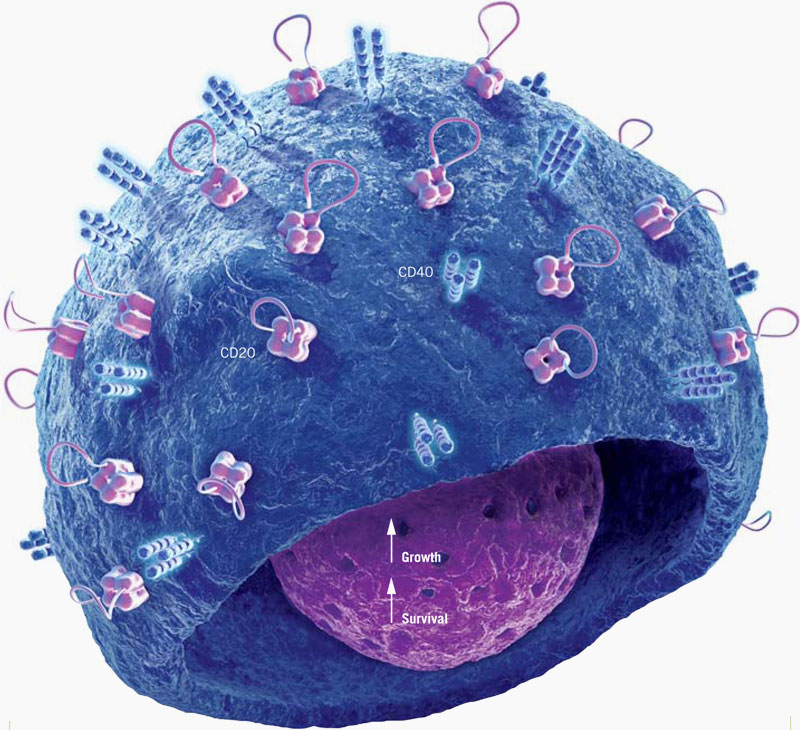
\includegraphics[height=50mm]{Cover/coverimage}  \end{center} % gráficos
    \vspace{5mm}

    %%% Titulo
    \centering
    \Large \textbf{Learnable Sparsity and Weak Supervision for Compact, Transparent, and Data Efficient Neural Models}
    % \\ \vspace{10mm}
    % \Large Optional Subtitle
    % \\ \vspace{15mm}
    \\ \vspace{25mm}  % NO SUBTITLE
    \large \textbf{Gonçalo Migueis de Matos Afonso Correia} \\
    \vspace{4cm}

    \begin{minipage}{\textwidth}
        \begin{tabularx}{\textwidth}{ l @{ } l }
            \textbf{Supervisor} :    & \textbf{Doctor} André Filipe Torres Martins, University of Lisbon \\
            \textbf{Co-Supervisor} : & \textbf{Doctor} Vlad Niculae, University of Amsterdam             \\
        \end{tabularx}

    \end{minipage}
    %
    %\vspace{27mm}
    \\ \vspace{20mm}
    \centering
    \large \textbf{Thesis specifically prepared to obtain the PhD Degree in}\\
    \large Electrical and Computer Engineering\\
    %\\ \vspace{2mm}
    \vspace{18mm}
    \Large \textbf{Draft}

    \vspace{15mm}

    %\large \textbf{\todaythesis\today} \\
    \large \textbf{April 2022} \\
    \let\thepage\relax
\end{flushleft}
\pagebreak
%\setcounter{page}{1} \pagenumbering{Alph}

% Add PDF bookmark 
\pdfbookmark[0]{Title}{Title}

%%% LOGO
\thispagestyle{empty}
\begin{flushleft} ~\\ \vspace{-12mm} \hspace{-12mm}  
\includegraphics[width=50mm]{Cover/istnewlogo} 
 
 %%% Instituição
\centering
\LARGE \textbf{Universidade de Lisboa \\ Instituto Superior Técnico}
%%% espaço sem gráficos
\vspace{30mm}

%%% Optional Image
%\vspace{10mm}
%~\\ \vspace{50mm} % gráficos
%\\ \begin{center} 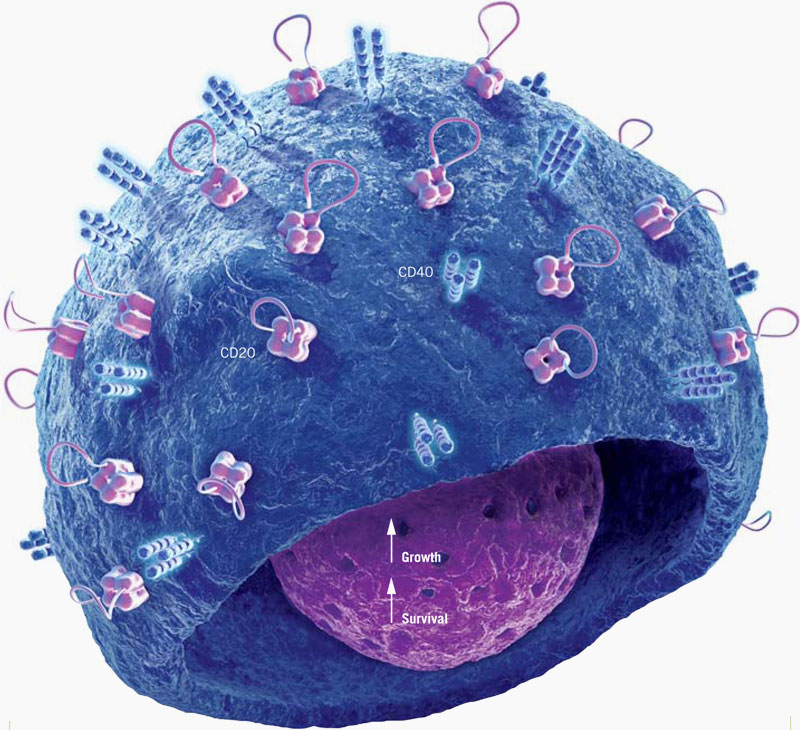
\includegraphics[height=50mm]{Cover/coverimage}  \end{center} % gráficos
 \vspace{5mm}
 
 %%% Titulo
\centering
\LARGE \textbf{Título da Tese que descreve o objeto de estudo.}
\\ \vspace{10mm}
\Large Subtítulo Opcional
\\ \vspace{15mm}
%\\ \vspace{25mm}  % NO SUBTITLE
\Large \textbf{Nome completo} \\
\vspace{4cm}

\begin{minipage}{\textwidth}
\begin{tabularx}{\textwidth}{ l @{ } l }
\large \textbf{Orientador} : & \textbf{Doutor} Nome completo\\
 \large \textbf{Co-Orientador} :  & \textbf{Doutor} Nome completo\\
 %&    ~~~~~~~~~~~~~~~~~~~~~~~~~~ large name\\
\end{tabularx}

\end{minipage}
%
\\ \vspace{27mm}
%\vspace{12mm}
\centering
\large \textbf{Tese especialmente elaborada para a obtenção do grau de Doutor em}\\
\large Engenharia Mecânica\\
%\\ \vspace{2mm}
\vspace{18mm}
\Large \textbf{Tese Provisória}
 
\vspace{15mm}

%\large \textbf{\todaythesis\today} \\
\large \textbf{November 2017} \\
\let\thepage\relax
\end{flushleft}
\pagebreak

%%-------------------------------------
\clearpage
% Since I am using double sided pages, the second page should be white.
% Remember that when delivering the dissertation, IST requires for the cover to appear twice.

\thispagestyle{empty}
\cleardoublepage

\setcounter{page}{1} \pagenumbering{roman} % --- Start with Roman numbering ---

\baselineskip 18pt % line spacing: -12pt for single spacing
%               -18pt for 1 1/2 spacing
%               -24pt for double spacingnts}

%%%% Initial Chapters
\selectlanguage{english}
\begin{abstract}

    Neural network models have become ubiquitous in Machine Learning
    literature. These models are compositions of differentiable
    building blocks that result in dense representations of the
    underlying data. To obtain good representations, conventional
    neural models require many training data points. Moreover, those
    representations, albeit giving a high performance on many tasks,
    are largely uninterpretable. These models are often
    overparameterized and give out representations that do not
    compactly represent the data. To address these issues, we find
    solutions in {\textbf sparsity} and various forms of {\textbf
            weak supervision}. For {\textbf data-efficiency}, we leverage
    transfer learning as a form of weak supervision. The proposed
    model can perform similarly to models trained on millions of data
    points on a sequence-to-sequence generation task, even though we
    only train it on a few thousand. For {\textbf transparency}, we
    propose a probability normalizing function that can learn its
    sparsity. The model learns the sparsity it needs differentiably
    and thus adapts it to the data according to the neural
    component's role in the overall structure. We show that the
    proposed model improves the interpretability of a popular machine
    translation neural architecture compared to conventional
    probability normalizing functions. Finally, for {\textbf
            compactness}, we uncover a way to obtain exact gradients of
    discrete and structured latent variable models efficiently. The
    discrete nodes in these models can compactly represent implicit
    clusters and structures in the data, but training them was often
    complex and prone to failure since it required approximations
    that rely on sampling or relaxations. We propose to train these
    models with exact gradients by parameterizing discrete
    distributions with sparse functions, both unstructured and
    structured. We obtain good performance on three latent variable
    model applications while still achieving the practicality of the
    approximations mentioned above. Through these novel
    contributions, we challenge the conventional wisdom that neural
    models cannot have these three properties.

\end{abstract}
\begin{keywords}
    Machine learning,
    natural language processing,
    neural networks,
    sparsity,
    latent variable models.
\end{keywords}
\clearpage
\thispagestyle{empty}
\cleardoublepage
\singlespacing
\selectlanguage{portuguese}
\onehalfspacing
\begin{resumo}

    Esta tese propõe novas técnicas para melhorar a eficiência na
    utilização de dados, a transparência e a compacidade de redes
    neuronais, com aplicações em processamento de linguagem
    natural. Graças aos nossos avanços em técnicas de
    esparsidade e supervisão fraca, desafiamos a doutrina de que
    modelos neuronais não são capazes de exibir tais
    características.

    Para atingir eficiência na utilização de dados, propomos
    aproveitar as capacidades de transferência de aprendizagem de
    redes neuronais pré-treinadas em tarefas sequenciais. Aplicamos o
    nosso método em Pós-Edição Automática (PEA) para demonstrar a sua
    eficácia. Para isso, usamos um modelo neuronal pré-treinado nos
    dois componentes principais do sistema de PEA, explorando várias
    estratégias de compartilhamento de parâmetros. Conseguimos obter
    resultados competitivos com modelos treinados em grandes
    quantidades de dados artificiais, mas treinando em apenas um
    pequeno conjunto de dados.

    Para atingir transparência, propomos substituir a função
    \textit{softmax} nos mecanismos de atenção de redes neuronais
    pela função \textit{$\alpha$-entmax}: uma generalização
    diferenciável da \textit{softmax} que permite que palavras com
    baixa pontuação recebam precisamente um peso de zero. Para além
    disso, derivamos um método para aprender o parâmetro $\alpha$
    automaticamente, que controla a forma e a dispersão da função
    \textit{$\alpha$-entmax}. Em tradução automática, mostramos que a nossa
    abordagem adaptativa melhora a interpretabilidade quando comparado
    à simples aplicação da \textit{softmax}.

    Para atingir modelos compactos, propomos uma nova técnica para
    treinar modelos com variáveis latentes discretas de forma mais
    eficaz. Treinar este tipo de modelos é muitas vezes desafiador devido
    à necessidade de usar estratégias de amostragem com variância alta,
    ou usar relaxamentos para o espaço contínuo. Em vez disso, propomos usar
    mapeamentos esparsos diferenciáveis para parametrizar as
    distribuições discretas. A esparsidade vai permitir uma marginalização eficiente como
    alternativa às técnicas mencionadas.
    Aplicamos o nosso método a três diferentes tarefas de modelos
    com variáveis latentes discretas e obtemos resultados competitivos
    atingindo, mesmo assim, a praticabilidade de aproximações
    baseadas em amostragem.

\end{resumo}

\begin{palavraschave}
    Aprendizagem automática,
    processamento de linguagem natural,
    redes neuronais,
    esparsidade,
    modelos com variáveis latentes.
\end{palavraschave}
\clearpage
\thispagestyle{empty}
\cleardoublepage

\pdfbookmark{Acknowledgments}{Acknowledgments}
\begin{acknowledgments}

    This thesis would not have been possible without the support of
    many. Family and friends have supported me over
    the years to various degrees.
    
    First of all, I dedicate this thesis to my mother, Maria da
    Conceição, and my father, Júlio António. I profusely thank them
    for everything they have done in my education, both academically
    and personally. I especially thank them for supporting me
    immediately after I told them that I wanted to pursue a Master's
    degree in Artificial Intelligence in Edinburgh, even though I had
    already started one in Biomedical Engineering. Through a domino
    effect, this has culminated in this thesis, and I hope I'm making
    them proud. I also want to thank my grandmother, Maria Helena, as she
    always cared for me as though I were her child. I'm also grateful
    to the rest of my family for their support and encouragement.
    
    This thesis would have been much harder to do, had I not had
    endless support from Sofia. She has been a pillar in my life
    throughout these years, and I'm glad to have her as my partner.
    Many ideas have blossomed from conversations with her over dinner
    or on the long walks we usually take. Moreover, she has drawn
    many of the figures present in this thesis (the reader can infer
    which ones by how much better they look).
    
    I am forever grateful to my official advisors, André and Vlad,
    and my honorary (but just as important) advisor, Wilker. They
    have been stellar, and I am fortunate to consider them not only
    advisors but also friends. I thank André for believing in me in
    the first place and inviting me to start on this journey with
    him. I thank Vlad for always looking out for me in numerous ways
    and inspiring me to be better. I thank Wilker for introducing me
    to latent and variational modeling, topics I was and am highly
    interested in, and for being kind and patient while explaining
    those concepts.
    
    I am fortunate to have had the help and support of many friends.
    From school, I thank João Miguel, Ricardo B., Martim, Sérgio,
    Álvaro, Inês, Alice, Leonor, Miguel, Filipe, Ricardo F., Renato,
    and Luciano. I've known many of them since I was six years old,
    and I hope to have you by my side for countless more years! From
    IST (2012-2016), I thank Catarina, Patrícia, Mariana, Maria,
    Miguel, Joana, Diogo, Gonçalo, André Melo, Daiane, and João. They
    are incredible friends and an endless source of laughs,
    inspiration, and kindness. From Edinburgh, I thank Alasdair,
    Antonio, Lasse, Diogo, and Miguel. We all shared great
    discussions and experiences over there, learned from among the
    best, and despite some physical distance right now, I still feel
    like we are close. I also thank my \textit{sis-law} Inês, for
    being the little sister I never had, and my \textit{bro-law}
    Francisco, who would undoubtedly find it extremely funny to be
    mentioned in a doctoral dissertation. A special thanks belongs to
    João Miguel, André Melo, and João Graça. When I was most confused
    and lost in my academic journey, they were the ones who persuaded
    me (thankfully!) to change paths and pursue a career in Machine
    Learning. This thesis exists, in a way, because of conversations
    with them.
    
    Finally, I'm grateful for my colleagues at the SARDINE and
    Probabll labs, who I'm glad to call friends. I thank Ben, Erick,
    Tsveti, Marcos, Pedro, Chryssa, Taya, Nuno, Patrick, António,
    Bryan, and Lina. This endeavor would have been so dull had not
    all of them been around, and countless discussions led to many
    ideas present in this thesis. Additionally, even though we have
    never met in person, I thank Mathieu Blondel, who had the idea to
    learn $\alpha$ in $\alpha$-\entmaxtext
    (\chapref{chap:adaptsparse}), and had done initial work on
    top-$k$ sparsemax (\chapref{chap:sparsemarg}).
    
    My PhD was funded by the European Research Council (ERC
    StG DeepSPIN 758969).
    
\end{acknowledgments}
\clearpage
\thispagestyle{empty}
\cleardoublepage

\thispagestyle{empty}
\hbox{} \vfill
\begin{flushright}
\small \textit{\textbf{Anyone who has never made a mistake has never tried anything new.}}
\\ \vspace{2mm}  
\scriptsize Albert Einstein
\end{flushright}

\clearpage
\thispagestyle{empty}
\cleardoublepage % --- Citation (optional) ---
%% Use Main document Language
\selectlanguage{english}
%% ------
% This is required for the fancy chapters
\dominitoc
\dominilof
\dominilot

%%%%%%%%%%%%%%%%%%%%%%%%%%%%%%%%%%%%%%%%%%%%%%%%%%%%%%%%%%%%%%%%%%%%%%
% List of contents
%\renewcommand{\baselinestretch}{1}
\pdfbookmark[0]{Index}{index}
\pdfbookmark[1]{Contents}{toc}
\tableofcontents
% \contentsline{chapter}{References}{\pageref{bib}}
\clearpage
\thispagestyle{empty}
\cleardoublepage
%\renewcommand{\baselinestretch}{1.5}
%%%%%%%%%%%%%%%%%%%%%%%%%%%%%%%%%%%%%%%%%%%%%%%%%%%%%%%%%%%%%%%%%%%%%%
% List of figures
\pdfbookmark[1]{List of Figures}{lof}
\listoffigures
\clearpage
\thispagestyle{empty}
\cleardoublepage

%%%%%%%%%%%%%%%%%%%%%%%%%%%%%%%%%%%%%%%%%%%%%%%%%%%%%%%%%%%%%%%%%%%%%%
% List of tables
\pdfbookmark[1]{List of Tables}{lot}
\listoftables
\clearpage
\thispagestyle{empty}
\cleardoublepage

% %%%%%%%%%%%%%%%%%%%%%%%%%%%%%%%%%%%%%%%%%%%%%%%%%%%%%%%%%%%%%%%%%%%%%%
% % List of algorithms
% Requires packages algorithmic, algorithm
% \pdfbookmark[1]{List of Algorithms}{loa}
% \listofalgorithms
% \cleardoublepage
\acresetall
%% Remain list of table titles are set manualy
%% %%%%%%%%%%%%%%%%%%%%%%%%%%%%%%%%%%%%%%%%%%%%%%%%%%%%%%%%%%%%%%%%%%%%%%
 % List of acronyms
\pdfbookmark[1]{List of Acronyms}{loac}
%\chapter*{Abbreviations}

%GLOSSARIO de Acrónimos
\printglossary[type=\acronymtype]

\clearpage
\thispagestyle{empty}
\cleardoublepage




\begin{notation}
    \begin{tabularx}{\textwidth}{r X}
        % \multicolumn{2}{l}{\textbf{Vectors, matrices, and indexing.}} \\

        $a$, $\bm{a}$, $\bm{A}$, and $\mathcal{A}$ & a scalar, a
        vector, a matrix, and a set, respectively;                                                                                                                            \\

        $v_i$                                      & the $i$th element of vector $\bm{v}$;                                                                                    \\

        $w_{ij}$                                   & the element on the $i$th row and $j$th column of
        $\bm{W}$;                                                                                                                                                             \\

        $\bm{e}_{i}$                               & the indicator vector for which every entry is
        zero, except the $i$\textsuperscript{th}, which is 1;                                                                                                                 \\

        $\simplex^K$                               & the canonical simplex, \ie, $\pv \in
        \reals^K:~\sum_i \xi_i = 1, \pv \geq \bm{0}\}$;                                                                                                                       \\

        $Y$                                        & a random variable;                                                                                                       \\

        $p_Y(y;\theta)$                            & the probability mass function (pmf) that
        specifies the probability distribution of the random variable
        $Y$, evaluated at the outcome $y$ using parameters $\theta$;                                                                                                          \\

        $p(y|x)$                                   & the probability value of outcome $y$ given outcome $x$;                                                                  \\

        $\text{Cat}(f(\cdot;\theta))$              & the categorical distribution parameterized by the function $f(\cdot;\theta)$                                             \\

        $\text{Cat}(y; f(x;\theta))$               & the probability mass value of outcome $y$ under the categorical distribution parameterized by the function $f(x;\theta)$ \\

        $\mathbb H(p)$                             & the Shannon's entropy of the pmf
        $p(z)$, \ie, $-\sum_i p_i \log p_i$;                                                                                                                                  \\

        $\KL\left[ p || q \right]$                 & the Kullback-Leibler divergence
        of $p(z)$ from $q(z)$;                                                                                                                                                \\

        $\|z\|_0 \defeq |\{t: z_t \neq 0 \}|$      & the number of
        non-zeros of a sequence $z$;                                                                                                                                          \\

        $\mathbb{E}_{p(z)}[f(z)]$                  & the expectation of a function
        $f:\ZZ \rightarrow \mathbb{R}$ under the pmf $p(z)$,
        letting $z \in \ZZ$ be an outcome of a random variable;                                                                                                               \\



        % $\bs{w}_j$ &
        %     the $j$th column of matrix $\bs{W}$; \\

        % $\bs{v}_{\mathcal{S}}$ &
        %     the sub-vector of $\bs{v}$ indexed by an
        %     ordered set $\mathcal{S} \subset  \mathbb{N}$; \\

        % $\bs{W}_{\mathcal{S}}$ &
        %     the sub-matrix of $\bs{W}$ consisting of the
        %     columns indexed by $\mathcal{S}$; \\

        % $[\bs{v}_1, \ldots,  \bs{v}_k]$ &
        %     vector concatenation, \ie, for $\bs{v}_i \in \real^{d_i},  
        %     [\bs{v}_1, \ldots, \bs{v}_k] \in \real^{\sum_i d_i}$; \\

        % $[\bs{W}_1, \ldots, \bs{W}_k]$
        %     & column-wise stacking of  $\bs{W}_i \in
        %     \real^{m\times d_i}$; $[\bs{W}_1,\ldots,\bs{W}_k]
        %     \in\real^{m\times\sum_i d_i}$; \\

        % $\range{n}$ &
        %     the index set, \ie, $\{ 1, 2, \cdots, n \}$ for $n\in\mathbb{N}$. \\

        %\multicolumn{2}{l}{\textbf{Important sets and functions.}} \\

        % $\iverson[\pi]$ &
        %     the Iverson bracket: $\iverson[\pi]=1$ if proposition $\pi$
        %     is true, $0$ otherwise; \\

        % $\norm{\bs{v}}_p$ &
        %     the $\ell_p$ norm of vector $\bs{v}\in\real^d$, \ie,
        %     $\norm{\bs{v}}_p = \left(\sum_{i=1}^d |v_i|^p \right)^{1/p}$; \\ 

        % $\Simplex^d$ &
        %     the canonical simplex, \ie, $\{\bs{y} \in \real^d,
        %     \norm{\bs{y}}_1 = 1, \bs{y} \succcurlyeq \bs{0} \}$;\\

        % $\id{\mathcal{S}}$ &
        %     the indicator function of set $\mathcal{S}$,
        %     $\id{\mathcal{S}}(\bs{x}) = 0$ if $\bs{x} \in \mathcal{S}$,
        %     else $+\infty$;\\

        % $\proj{\mathcal{S}}(\bs{v})$ &
        %     euclidean projection of $\bs{v}$ onto the set $S$, \ie, 
        %     $\displaystyle \argmin_{\bs{y} \in S} \norm{\bs{v}-\bs{y}}_2^2$; \\[-0.5em]

        % $\bar{\real}$ &
        %     extended real numbers, \ie, $\real \cup \{+\infty\}$ \\

        % $\dom f$ &
        %     the domain of function
        %     $f:\real^d\rightarrow\bar\real$, \ie, $\left\{\bs{x}\in\real^d:
        %     f(\bs{x}) < \infty \right\};$\\

        % $\partial f(\bs{x})$ &
        %     the subdifferential of convex function $f:\real^d \rightarrow
        %     \bar{\real}$ at point $\bs{x}$, \ie, $\partial f(\bs{x})=\left\{
        %     \bs{g} \in \real^d: \forall \bs{z} \in \dom f,
        %     f(\bs{z}) \geq f(\bs{x}) + \bs{g}^\tr(\bs{z}-\bs{x})\right\}$;
        %     its elements $\bs{g}\in\partial f(\bs{x})$ are called
        %     \emph{subgradients} of $f$ at $\bs{x}$; \\

        % $\nabla f(\bs{x})$ &
        %     the gradient of differentiable $f$ at $\bs{x}$, \ie, $\partial
        %     f(\bs{x})=\{\nabla f(\bs{x})\}$; \\

        % $\bs{J_h}(\bs{x})$ &
        %     the Jacobian of $\bs{h}:\real^d\rightarrow\real^m$, \ie, 
        %     $\bigl(\bs{J_h}(\bs{x})\bigr)_{ij}=\pfrac{h(\bs{x})_i}{x_j}$; \\

        % $\bs{H}_f(\bs{x})$ &
        %     the Hessian of $f:\real^d\rightarrow\real$, \ie,
        %     $\bigl(\bs{H}_f(\bs{x})\bigr)_{ij}=\pfrac{^2 f(\bs{x})}{x_i x_j}$; \\
    \end{tabularx}
\end{notation}

%% Use Main document Language
\selectlanguage{english}
% Pages number is starting now with arabic style... until now it was on roman mode
\pagenumbering{arabic} \setcounter{page}{1}
\baselineskip 18pt
%% Define the title of Chapter Table of Contents
\mtcsettitle{minitoc}{Contents}
%% ------
\pagestyle{documentsimple}%Simple head
% %%%%%%%%%%%%%%%%%%%%%%%%%%%%%%%%%%%%%%%%%%%%%%%%%%%%%%%%%%%%%%%%%%%%%%
% The Introduction:
% %%%%%%%%%%%%%%%%%%%%%%%%%%%%%%%%%%%%%%%%%%%%%%%%%%%%%%%%%%%%%%%%%%%%%%
\fancychapter[Introduction]{Introduction}
\label{cap:int}

\cleardoublepage
\doublespacing

\noindent Deep learning is a field of machine learning that uses
\textbf{neural networks} to learn and obtain predictions
and inferences from unprocessed data. The success of well-known deep
learning models~\citep[\textit{inter
        alia}]{convnet,devlin2018bert,brown2020language} relies on a rich
parameterization accomplished through the use of numerous layers of
computation. Along with vast amounts of data points,
such heavy parameterization allows these models to learn good
vector representations that permit them to excel in their respective
tasks. However, these models are often highly overparameterized;
additionally, their interpretation is difficult due to the underlying
opaqueness of neural models. Moreover, they require costly computing
power, which causes environmental concerns~\citep{Strubell2019}. In
natural language processing (NLP), one such model is the transformer
architecture~\citep{vaswani2017attention} which has quickly risen to
prominence thanks to its outstanding performance, leading to
improvements in the state-of-the-art of neural machine
translation~\citep[NMT;][]{marian,ott2018scaling}, and served as an
inspiration to even bigger and more powerful general-purpose models
like BERT~\citep{devlin2018bert} and
\mbox{GPT-3}~\citep{brown2020language}.

On the other hand, neural latent variable models are powerful and
expressive tools for finding patterns in high-dimensional data, such
as images or text~\citep{Kim2018,Kingma+2014:VAE,RezendeEtAl14VAE}.
These models have powerful structural biases that guide the model's
training; of particular
interest are \emph{discrete} latent variables, which can recover
categorical and structured encodings of hidden aspects of the data,
leading to compact representations~\citep{KingmaEtAl2014SSVAE} and,
in some cases, superior explanatory power~\citep{titov2008joint,
    Bastings2019}. However, more often than not, training models with
discrete latent nodes is a difficult task due to the need to rely on
high-variance methods~\citep{Williams1992} or relaxations into the
continuous space~\citep{GumbelSoftmax,Concrete}.

In this thesis, we will address the issues mentioned above of overuse
of data points, opaqueness, and the difficulties in training compact
versions of neural models. To obtain the solutions presented, we will
rely on forms of \textbf{weak supervision} and, most importantly, on
\textbf{sparse} projections onto probability spaces.

When this project began in 2018, the use of large pre-trained
language models was very much in an infant state.
ELMo~\citep{peters2018deep} had just been released, closely followed
by BERT~\citep{devlin2018bert}, and practitioners were just starting
to use these models in their research to improve the state-of-the-art
of tasks in NLP. The transformer
arquitecture~\citep{vaswani2017attention} was also a promising model
that had just started to pick up much steam and to replace the
recurrent neural network (RNN) sequence-to-sequence models that were
prominent in the NLP literature at the
time~\citep{bahdanau2014neural}. During the course of this project,
there has been remarkable progress in neural networks and NLP
research; for example, pre-trained language model literature has
evolved from proposing simply encoders that provide rich contextual
representations~\citep{devlin2018bert}, to also provide decoders that
deliver extremely realistic text~\citep[GPT-3;][]{brown2020language},
and encoder-decoder models that allow for any task to be posed as a
natural language
prompt~\citep{raffel2020Exploringlimitstransfer,lewis2020BARTDenoisingSequencetoSequence}.

The approaches found in the present thesis are, in part, a product of
the aforementioned research efforts. As we will see in the following
chapters, we introduced a way to use large pre-trained encoders in
generation tasks before large pre-trained decoder and encoder-decoder
models were developed; we tackled the opaqueness of the, at the time,
recently proposed and barely understood transformer architecture; and
pioneered a new paradigm in discrete latent variable model training.

We also note that this thesis has strong roots in a line of
literature that has been proposing new methods to induce sparsity
within the computational graphs of neural networks. Before this
thesis, the foundations had been laid by the study of sparse
normalization functions~\citep{sparsemax,fusedmax,entmax} and their
applications~\citep{maruf2019selective,malaviya2018sparse}, and also
their uses in structured
prediction~\citep{sparsemap,sparsemapcg}. During the
course of this project, we have extended this line of work by
tackling some of the abovementioned issues with our sparsity-induced
solutions. We have also created new foundations for others to extend
upon our work and create their own sparse approaches to new and
challenging problems~\citep{treviso2021PredictingAttentionSparsity,
    farinhas2022SparseCommunicationMixed}.

\section{Contributions and Thesis Statement}
\label{sec:int_contributions}

\noindent We will now summarize the contributions of this thesis, which will
address the open questions left to answer in the previous section.

\begin{itemize}

      \item \textbf{We use weak supervision by leveraging transfer learning
                  for data-efficient sequence-to-sequence models.} We show how to
            leverage a pre-trained encoder to perform a
            sequence-to-sequence task on a tiny dataset. We explore different
            avenues of parameter sharing and initialization to make this
            possible.


      \item \textbf{We propose a new deep model with attention that can
                  dynamically adapt to be denser or sparser as needed.} We change the
            transformer architecture such that each attention head, the main
            building block of transformers, can dynamically change its sparsity
            during training. This way, each attention head can accommodate its
            sparsity to its role in the overall model. To achieve that, we derive
            the gradient of $\alpha$ in $\alpha$-\entmaxtext{}~\citep{entmax}, a
            function akin to softmax, in which the sparsity of the probability
            vector is controlled by a parameter $\alpha$.

      \item \textbf{We conduct an extensive analysis on the increased
                  transparency of transformer models that use {\boldmath
                              $\alpha$}-\entmaxtext{} as its normalization function in the
                  attention mechanism.}
            Besides studying the distribution of sparsity and respective $\alpha$ values
            throughout all attention heads in the transformer, we also identify
            examples of sharper attention head behavior than what was found in
            previous work, along with the disentanglement of newfound behaviors
            thanks to our proposed sparsity.

      \item \textbf{We propose a new method to train discrete and
                  structured latent variable models based on the efficiency of
                  marginalizing expectations using sparsity.} Thanks to this method, we
            can train these families of latent variable models without recurring
            to any sampling or relaxations of the discreteness into
            the continuous space. In particular, in the unstructured case, our
            method relies on the sparsemax~\citep{sparsemax} projection function.
            In the structured case, we propose to either use
            SparseMAP~\citep{niculae2018sparsemap} or the novel top-$k$
            sparsemax.

      \item \textbf{We provide open-source code for each of the
                  methods we have proposed.}
            The respective repositories can be found in each
            of the chapters.


\end{itemize}

\paragraph*{Thesis Statement.} The primary claim of this thesis is
that, unlike what numerous previous works insist, neural
models have the capability of being data-efficient, transparent, and
compact: one only needs to look through a different lens that is
capable of leveraging weak supervision, sparsity, and latent
representations. We conclude that a \textit{vanilla}
application of neural models to the problem at hand is not sufficient
for achieving these properties: for \textbf{data-efficiency}, we find that we need
to allow parameter sharing, careful initialization, and powerful
transfer learning capabilities to succeed at a low-resource
generation task; for \textbf{transparency}, we can allow the model to have
sparsity and let it learn it according to its needs at training time; and
for \textbf{compactness}, we can leverage discrete latent variable models in a
better way than what was previously possible by using an exact but
efficient gradient.

\section{Publications}
\label{sec:int_publications}

This thesis is based, in part, on the following publications:

\begin{sloppypar}
      \begin{itemize}

            \item {\bf A Simple and Effective Approach to Automatic
                  Post-Editing with Transfer Learning}~\citep{Correia2019}.
                  Described in \chapref{chap:ape}, this paper was accepted as a
                  poster at ACL 2019.
                  
            \item {\bf Unbabel's Submission to the WMT2019 APE Shared Task:
                  BERT-based Encoder-Decoder for Automatic
                  Post-Editing}~\citep{lopes2019unbabels}. Not included as a specific
                  chapter within this thesis, this work describes an Automatic
                  Post-Editing model that was submitted to the APE Shared Task at
                  WMT2019. This model won the Shared Task, obtaining state-of-the-art
                  in APE at the time.
                  
            \item {\bf Adaptively Sparse
                  Transformers}~\citep{correia2019adaptively}. Described in
                  \chapref{chap:adaptsparse}, this paper was accepted for an oral
                  presentation at EMNLP 2019.
                  
            \item {\bf Efficient Marginalization of Discrete and Structured
                  Latent Variables via Sparsity}~\citep{correia2020procneurips}.
                  Described in \chapref{chap:sparsemarg}, this work was
                  accepted as a spotlight paper at NeurIPS 2020.
                  
      \end{itemize}
\end{sloppypar}
\section{Roadmap}
\label{sec:int_roadmap}

Herein we show the outline of the remainder of this thesis.

We begin in \chapref{chap:background} by reviewing major concepts
that are essential to understand the content of this thesis,
particularly neural network models for NLP, sparse probability
normalization functions, and latent variable models.

In \chapref{chap:ape}, we develop a sequence-to-sequence model for
Automatic Post-Editing using the Transformer architecture and by
harnessing the transfer learning power of a pre-trained large
language model.

In \chapref{chap:adaptsparse}, we augment the Transformer to use
attention modules that allow sparse probabilities that adaptively
change their own sparsity depending on their role within the model.

In \chapref{chap:sparsemarg}, we propose a new training method of
discrete and structured neural latent variable models, which uses
sparse probabilities in order to compute the training objective of
these models, instead of using Monte Carlo methods.

Finally, in \chapref{chap:conclusions}, we summarize the
contributions of the present thesis, address some of the limitations
and open problems of the present work, and discuss exciting future
directions of further research.


\cleardoublepage
\singlespacing

\fancychapter[Background]{Background}
\label{chap:background}

\cleardoublepage
\doublespacing

\noindent This chapter will discuss the foundations of our work and
remind the reader of crucial concepts needed to understand this
thesis. Foremost, we will present key machine learning concepts.
Then, we will discuss neural networks in the context of NLP,
particularly sequence modeling. Secondly, we will lay the foundations
for using unstructured and structured sparse projections into the
simplex in neural networks. Finally, we will discuss critical
concepts regarding latent variable models, particularly with discrete
(unstructured and structured) latent assignments.

\section{Machine Learning}
\label{sec:ml-primer}

\noindent We begin by presenting the main ingredients in the machine learning pipeline:
%
\begin{itemize}
    \item a dataset $\mathcal{D}$, made out of
          \textit{inputs} $\mathcal{D}=\left\{\bm{x}_n\right\}_{n=1}^N$ or
          \textit{input-output} pairs
          $\mathcal{D}=\left\{(\bm{x}_n,y_n)\right\}_{n=1}^N$;
    \item a set of parameters $\theta$;
    \item a loss function $L$.
\end{itemize}
%
With these ingredients, we create a machine learning pipeline by
taking a \textit{training set} that is a subset of $\mathcal{D}$ and estimate
the parameters $\theta$ by minimizing the loss
$L$ on that set. The resulting model with optimal
$\hat{\theta}$ can then be evaluated on a held-out set of
$\mathcal{D}$, called \textit{test set}, to assess its performance.
We will often assume $\mathcal D$ is made out of input-output pairs,
unless specified otherwise.

When the model is probabilistic, this process creates a probability
model that identifies the probability measure of a random experiment:
it maps from available inputs in the set of possible inputs
$\mathcal{X}$ to a probability distribution of a random variable $Y$. When the set of
possible outputs $\mathcal{Y}$ is discrete, the probability
distribution of $Y$ is prescribed by a probability mass function
(pmf) $p_{Y|X}(y|\bm{x};\theta)$; when the set of possible outputs
$\mathcal{Y}$ is continuous, the probability distribution of $Y$ is
prescribed by a probability density function (pdf). In the context of
the present thesis, we will not have applications in which
$\mathcal{Y}\in\reals$ (\ie, \textit{regression problems}) and as
such, when referring to $p_{Y|X}(y|\bm{x};\theta)$, we assume that it is a
probability mass function. Furthermore, our problems will most often
involve a $k$-way classification, and so $p_{Y|X}(y|\bm{x};\theta)$ will be
specifying a \textit{Categorical} distribution,
%
\begin{equation}
    Y|X\!\!=\!\bm{x}~\sim \text{Cat}(f(\bm{x}; \theta)),
\end{equation}
%
where $f(x; \theta) \in \simplex^{K-1}$ is a function such that
$p_{Y|X}(y|\bm{x};\theta)=\text{Cat}(y|f(\bm{x}; \theta))$.

\paragraph*{Supervised learning.} We now turn our attention to applications
in which one uses a dataset of input-output pairs. In such a case,
to estimate $\theta$ we minimize the loss over the input-pair dataset,
%
\begin{equation}
    \hat{\theta} = \argmin_\theta L_\mathcal{D}(\theta),
\end{equation}
%
where $L_\mathcal{D}(\theta)$ is the loss function:
the \textit{negative log-likelihood}
%
\begin{equation}
    L_\mathcal{D}(\theta) = -\mathcal{L}_\mathcal{D}(\theta) =
    - \sum_n \log p_{Y|X}(y_n|\bm{x}_n; \theta).
    \label{eq:discr-loss}
\end{equation}
%
A model with the loss function of \eqnref{eq:discr-loss} is called a
\textit{discriminative model}, while one that models instead
$p_{XY}(\bm{x}, y; \theta)$ is called a \textit{generative model}.
Typically, the loss function might also entail a regularization term (\eg, the $\ell_2$ norm),
which is added to the negative log-likelihood
%
\begin{equation}
    L_\mathcal{D}(\theta) = -\mathcal{L}_\mathcal{D}(\theta) + \mathcal{R}(\theta).
\end{equation}
%
Sometimes, instead of the probabilistically-grounded negative
log-likelihood, practitioners might use a non-probabilistic loss $\ell$ and
still use a statistical model; for example, one might use the 0/1
loss where the loss is $1$ if the $\argmax$ mode is wrong (\ie,
$\hat{y}\neq y$) and $0$ otherwise. After training the model, we wish
to make predictions $\hat{y}$ for each novel input $\bm{x}$ of the
test set, and we can make such predictions by using the optimal
trained parameters $\hat{\theta}$ and selecting, for instance, the highest-scoring
$y\in\mathcal{Y}$ by taking the $\argmax$
%
\begin{equation}
    \hat{y}=\argmax_{y\in\mathcal{Y}}p_{Y|X}\left(y|\bm{x};\hat{\theta}\right).
\end{equation}
%
For example, in a binary sentiment classification problem of English
sentences, $\mathcal{Y}=\{\text{negative},\text{positive}\}$, and
$\mathcal{X}$ would be the set of possible sentences in the English
language.

\paragraph*{Unsupervised learning.} Similarly, there are also applications in machine learning where we use just a
dataset of inputs $\mathcal D = \left\{\bm{x}\right\}_{n=1}^N$ and estimate the parameters $\theta$ under a loss to
obtain an unsupervised model; that is, a model in which inferences are made
without access to any labels (\ie, outputs). In this case, the loss function $L$ only
depends on the inputs $\bm{x}_n$ and the parameters $\theta$
and we thus model $p_X(\bm{x}|\theta)$.
In this case, the loss function is
%
\begin{equation}
    L_\mathcal{D}\left(\theta\right)=-\sum_n\log p_X\left(\bm{x}_n|\theta\right).
\end{equation}
%
In this setting, to assess the resulting model's performance,
we often compute the log-likelihood of the model under the test set
%
\begin{equation}
    \mathcal{L}_{\mathcal{D}_\text{test}}(\hat{\theta}) =
    \sum_n\log p_X\left(\bm{x}_n|\hat{\theta}\right),
\end{equation}
%
that is, we assess the likelihood of the model being able to generate
the data points $\bm{x}$.

\paragraph*{Semi-supervised and weakly-supervised learning.} In a
semi-supervised setting, there is typically a smaller portion of the
dataset that is labeled,
$\mathcal{D}_{L}=
    \left\{(\bm{x}_n,y_n)\right\}_{n=1}^{N_{L}}$,
and the remaining majority is unlabeled,
$\mathcal{D}_{U}=
    \left\{(\bm{x}_n)\right\}_{n=1}^{N_{U}}$.
The parameters are then estimated by using a combination of losses: a
component that is supervised and another that is unsupervised.
Taking the loss examples given above, a probabilistic semi-supervised model could
have the loss function
%
\begin{equation}
    L_{\mathcal D}\left(\theta\right)=
    -\sum_{\bm{x}\in\mathcal{D}_U}
    \log p_{X}\left(\bm{x}|\theta\right)
    -\sum_{(\bm{x},y)\in\mathcal{D}_L}
    \log p_{XY}\left(\bm{x}, y;\theta\right).
    \label{eq:semisup}
\end{equation}
%
In some applications,
both models may be independent components that share some
parameters; in others, they are components of the same joint distribution over
$\mathcal{X}\times\mathcal{Y}$.
In the context of this
thesis, we will use the term \textit{weakly-supervised} and
\textit{weak supervision} to refer to a broader setting that aims to
alleviate the need for labeled data to obtain a well-performing
model. This setting not only includes semi-supervision but also
includes, for example, the transferring of learned parameters of an
already optimized unsupervised model to a supervised one, also called
\textit{transfer learning}. In such a case, the estimation of
parameters can first occur by minimizing the first loss component in
\eqnref{eq:semisup}, and then those learned parameters can be reused
as an initialization on the minimization of the second component.
While not explored in this thesis, other forms of weak supervision
include the usage of underspecified or unreliable labels, linguistic
constraints, labels obtained via heuristics, among others.

\subsection{Linear and Deep Models}

\noindent Naturally, there are many different ways one can use $\theta$ to
parameterize $p_{Y|X}\left(y|\bm{x};\theta\right)$. One of the simpler ways
is to define a log-linear model
%
\begin{align}
    p_{Y|X}\left(y|\bm{x};\theta\right) & = \text{Cat}(y|f(\bm x; \theta)) \\
    f(x; \theta)                        & = \softmax \left(\bm{s}\right)   \\
    \bm{s}                              & 
    = \bm{W}_{\theta}^T\bm{\phi}\left(\bm{x}\right) \label{eq:linear}
\end{align}
%
where $\bm{\phi}$ is a function that maps $\bm{x}$ into a
manageable space, $W_{\theta}$ is a matrix of learnable weights, and
\textbf{softmax} is a function that maps a vector of scores $\bm{s}\in\reals^K$ into
a ``vector of probabilities'', that is, $\sum_{k=1}^K\left[\softmax(\bm{s})\right]_k=1$
and $\left[\softmax(\bm{s})\right]_k \geq 0$.

\begin{definition}[softmax]
    The mapping function \textbf{softmax} is defined as
    \begin{equation}\label{eq:softmax}
        \left[\softmax(\bm{s})\right]_j = \frac{\exp(s_j)}{\sum_{j'} \exp(s_{j'})}.
    \end{equation}
\end{definition}

In these linear models, the problem of obtaining the optimal $\bm{W}_{\theta}$ lies
within the set of problems that convex optimization can solve, which
significantly simplifies the optimization process. While the
optimization simplicity of linear models is appealing, constructing a suitable
$\bm{\phi}$ may require significant effort. The creation of an
effective feature function $\bm{\phi}: \mathcal{X} \rightarrow \reals^d$ might
demand extensive knowledge of the domain of $\mathcal{X}$ and of the
task itself. The \textit{art} of creating these functions $\bm{\phi}$
is often called \textbf{feature engineering}.

An alternative to the log-linear model is a \textbf{neural network}, which, in a
way, performs feature engineering automatically through the use of hidden
representations. Neural networks use non-linear functions, also known
as \textit{activation functions}, along with linear functions similar
to \eqnref{eq:linear} in order to build these hidden representations.

\begin{definition}[neural network]
    A neural network with parameters $\theta$ is a function
    composed of building blocks that comprise both linear and non-linear
    functions. These building blocks are called \textit{layers}.
    The layers connect in a sequence, and the output of each
    layer is fed into the next layer. The output of the last layer is
    the output of the neural network
    %
    \begin{equation}
        f(x; \theta) = \pi 
        \left(\bm{W}_{\theta}^T\bm{\phi}_{\theta}\left(\bm{x}\right)\right)\,,
    \end{equation}
    %
    where compositions of differentiable functions with learnable
    $\theta$ parameterize $\bm{\phi}_{\theta}$ and $\pi$ is a
    function that projects the scores into vectors of probabilities (\eg, softmax).
    The composition of $\bm{\phi}_{\theta}$ is extremely flexible and
    can be defined in a variety of ways, making it a powerful way to
    obtain meaningful representations of the input space.
\end{definition}
%
Thanks to its non-linearities, neural networks effectively create
intermediate abstractions of the data, which are optimized to represent the data
more effectively in order to succeed at the task, bypassing the need
for feature engineering.

Just as well, non-linearities and the flexible composition of functions end up
impeding the usage of convex optimization, and so neural networks are
often trained instead through a process called
\textit{backpropagation}, a gradient-based optimization algorithm.

\begin{definition}[backpropagation]
    Backpropagation is a gradient-based optimization algorithm that
    locally minimizes the loss function $L$ by iteratively updating the
    parameters $\theta$. In order to be able to update $\theta$,
    the only requirement is to be able to compute the gradient of
    $L$ with respect to every coordinate $\theta_d\in\theta$:
    %
    \begin{equation}
        \frac{\partial L_{\mathcal{D}}(\theta)}{\partial \theta_d}.
        \label{eq:backprop}
    \end{equation}
    %
\end{definition}

Due to the simplicity of this requirement, practitioners can build
neural networks in a modular way, where differentiable building
blocks of functions are combined in arbitrary computational graphs. A
handful of different algorithms can be used to update $\theta$ during
backpropagation; for example, Adam~\citep{kingma2014adam}.

In practice, computing \eqnref{eq:backprop} for the whole dataset
$\mathcal D$ is a costly operation, and so the gradient is usually
computed through an unbiased estimate: independent and identically
distributed samples of the dataset are drawn at each iteration, and \eqnref{eq:backprop}
is computed on that set of samples (\ie, the \textit{mini-batch}).
The size of the step at which $\theta$ is updated is determined by a value usually called the learning rate,
which is a hyperparameter of the model that is chosen to maximize a given metric on a held-out
dataset (the \textit{validation set} or \textit{development set}).

\section{Neural Networks and Natural Language}

\noindent Using neural networks in NLP applications is a pivotal part
of the research shown in the present thesis. While there are many
ways of applying neural networks to NLP, exploiting many different
architectures and aimed at many different tasks, we give
special attention to sequence-to-sequence models, which we will
explain in the sequel.

Nevertheless, in the context of neural networks for NLP, there is a
clear focus on obtaining vectorized representations of words, of words
within their context, and of whole sentences. A common ingredient in all
neural network architectures of NLP is the use of
\textbf{embeddings}. After the sentence is segmented into tokens
(words, segments of words, and punctuation), the first component of the
neural network is an \textit{embedding table}: a set of learnable
vectors of parameters that represent each token in the vocabulary $V$
(chosen beforehand). For each token in the sentence, the
corresponding vector (\textit{embedding}) is taken from the table,
and the resulting output is the sequential concatenation of
embeddings. Many different architectures can extend the computational
graph afterward, which will change those representations and entangle
them to contextualize the representation of each word in the context
of the sentence and the task at hand.

\subsection{Sequence-to-Sequence Models}

\noindent In NLP, predicting the next word in a sentence is a common
task, for example in problems such as machine translation (MT). The
broader family of models that handle such tasks are sequential
models. In this thesis, we mainly focus on
\textbf{sequence-to-sequence models}.

\begin{definition}[sequence-to-sequence models]
    A sequence-to-sequence model (\textit{seq2seq}) is a model that takes as input a
    sequence of tokens and produces as output another sequence of tokens.
    The model has $Y_i | Y_{\leq i}, X \sim \text{Cat}(f(y_{\leq i}, \bm{x};
        \theta))$ as its underlying distribution. In turn, the pmf
    %
    \begin{equation}
        p(y_i|y_{\leq i}, \bm{x}) = \text{Cat}(y_i|f(y_{\leq i}, \bm{x}; \theta))
    \end{equation}
    %
    specifies that probability distribution, where
    $\bm{x}=[x^1, \dots, x^N]$ is the input sequence of words,
    $y_i$ is the next word in the output sequence $y=[y^1, \dots, y^M]$,
    and $y_{\leq i}$ is the history of previous words in $y$.
    When modeled with neural networks, these models typically have
    two main building blocks: the \textit{encoder}, which processes $\bm{x}$,
    and the \textit{decoder}, that parameterizes the probability of the next
    token $y_i$ in the context of $y_{\leq i}$ and $\bm{x}$.
\end{definition}

In the following section, we will expand on the architecture used in
the sequence-to-sequence models presented in this thesis: the \textbf{transformer}.

\subsection{Transformer}
\label{sec:transformer_bg}

\noindent The transformer~\citep{vaswani2017attention} is an architecture which
maps an input sequence to an output sequence through many layers of
\textbf{multi-head attention} mechanisms, yielding a dynamic,
context-dependent strategy for propagating information within and
across sentences. It contrasts with previous seq2seq models for neural machine translation (NMT), which
usually rely either on gated recurrent operations~\citep[often
    LSTMs:][]{bahdanau2014neural,luong2015effective} or static
convolutions~\citep{convseq}.

Attention mechanisms compute, for each query, a weighted
representation of the items. The particular attention mechanism used
in \citet{vaswani2017attention} is called \emph{scaled dot-product
    attention}.

\begin{definition}[attention mechanisms and scaled dot-product attention]
    Attention mechanisms are a possible differentiable building block
    of a neural network, mainly used in sequence modeling. For each
    item in the sequence, the attention mechanism computes a weighted
    representation of all the other items in said sequence or a given
    context sequence. Given the current item, it can often be
    interpreted as showing each item's importance in the context. A
    scaled dot-product attention mechanism is a particular type of
    attention mechanism:
    %
    \begin{equation}
        \att(\bm{Q}, \bm{K}, \bm{V}) = \amap
        \left(\frac{\bm{Q}\bm{K}^\tr}{\sqrt{d}}\right) \bm{V},
        \label{eq:att_scaled_dot}
    \end{equation}
    %
    where, given $n$ query contexts and $m$ sequence items under
    consideration, $\bm{Q} \in \reals^{n \times d}$ contains
    representations of the queries, $\bm{K}, \bm{V} \in \reals^{m
            \times d}$ are the \emph{keys} and \emph{values} of the items
    attended over, and $d$ is the dimensionality of these
    representations. The $\amap$ mapping normalizes row-wise using a mapping function like
    \textbf{softmax}, that is, $\amap(\bm{Z})_{ij} = \softmax(\bm{z}_i)_j$.
    In words, the \emph{keys} compute a relevance score between each item
    and query. Then, $\amap$ normalizes these attention weights, and
    these will weight the \emph{values} of each item at each query
    context.
\end{definition}

However, for complex tasks, different parts of a sequence may be
relevant in different ways, motivating \emph{multi-head attention} in
transformers. Multi-head attention is simply the application of
\eqnref{eq:att_scaled_dot} in parallel $H$ times, each with a
different learned linear transformation that allows specialization,
%
\begin{equation}\label{eq:head}%
    \ath_i(\bm{Q}\!,\!\bm{K}\!,\!\bm{V})\!=\!\att(\bm{QW}_i^Q\!\!,\bm{KW}_i^K\!\!,\bm{VW}_i^V\!).
\end{equation}

In the transformer, there are three separate multi-head attention mechanisms for
distinct purposes:
%
\begin{itemize}
    \item \textbf{Encoder self-attention:} builds rich, layered representations of
          each input word by attending to the entire input sentence;
    \item \textbf{Context attention:} selects
          a representative weighted average of the encodings of the input words at each
          time step of the decoder;
    \item \textbf{Decoder self-attention:} attends over the partial output sentence
          fragment produced so far.
\end{itemize}
%
Together, these mechanisms enable the contextualized flow of information between
the input sentence and the sequential decoder.

\subsection{Large Pre-trained Language Models}
\label{sec:pretrained-bg}

\noindent A recently attractive way to obtain high-performing models in NLP is
to use a pre-trained language model. These are models with many
parameters, trained on millions of sentences gathered from
the web, using many computational resources in the training process.
Many such models are publicly released and are
available for the research and industry community to use. Typically,
practitioners download an already optimized model from the web and
train it further by \textit{finetuning} it, that is, taking an
already trained model's parameters and optimizing them on a new
dataset, usually using a lower learning rate, such that the new
optimum does not veer too far from the original optimum.

Many different models have been released in the last few years, such
as ELMo~\citep{peters2018deep}, OpenAI GPT
series~\citep{radford2018improving, brown2020language},
BERT~\citep{devlin2018bert}, and
T5~\citep{raffel2020Exploringlimitstransfer}. Of particular interest
in this thesis is BERT since it is the model used in
\chapref{chap:ape}.

BERT, at its core, is a transformer model, as described in
\secref{sec:transformer_bg}. However, it is only made out of the
encoder building block and thus does not have language modeling
capabilities in its \textit{vanilla} form. As is the case with other
similar models, BERT was trained on an enormous corpus of sentences
in monolingual English and in multilingual datasets of 100+
languages. BERT's masked language modeling objective (MLM) has proven
to be a powerful mechanism to learn transferrable contextual encoder
representations of tokens and sentences. Many works have analyzed
the BERT model and have developed variants for it. Its study has even
been referred as ``BERTology''~\citep{rogers2020PrimerBERTologyWhat}.

\section{Sparsity and Structured Sparsity in Probability Distributions}
\label{sec:sparsity_background}

\subsection{Foundations}

\subsection{Sparsemax}\label{sec:sparsemax_bg}

The sparsemax mapping~\citep{martins2016softmax}, is given by the unique solution to
\begin{equation}\label{eq:sparsemax}
    \sparsemax(\s) \coloneqq \argmin_{\pv \in \simplex^K} \| \pv - \s \|_2^2\,.
\end{equation}

Like softmax, sparsemax is differentiable and has efficient forward and backward
passes~\citep{Held1974,martins2016softmax}, described in detail below;
the backward pass is essential in our use case. Since
\eqnref{eq:sparsemax} is the Euclidean projection operator onto the probability
simplex, and solutions can hit the boundary, sparsemax is likely to assign {\bf
        probabilities of exactly zero}; in contrast, softmax is always dense.

As a projection onto a polytope, the solution is likely to fall on the
boundaries or the corners of the set. In this case, points on the boundary of
$\simplex^K$ have one or more zero coordinates. In contrast, $\softmax(\s)
    \propto \exp(\s)$ is always strictly inside the simplex.
From the optimality conditions of the sparsemax problem~\eqref{eq:sparsemax},
it follows that the solution must have the form:
\begin{equation}\label{eq:sparsemax_form}
    \sparsemax(\s) = \max(\s - \tau, 0)\,,
\end{equation}
where the maximum is elementwise, and $\tau$ is the unique value that
ensures the result sums to one.
Letting $\bar{\ZZ}$ be the set of nonzero coordinates in the solution,
the normalization condition is equivalently
\begin{equation}
    \tau = \frac{\sum_{z \in \bar{\ZZ}} \ss_z}{|\bar{\ZZ}|}\,.
\end{equation}
Observing that small changes to $\s$ almost always have no effect on the support
$\bar{\ZZ}$, differentiating Equation~\ref{eq:sparsemax_form} gives
\begin{equation}
    \pfrac{\bar{\pv}}{\bar{\s}} = \bm{I}_{|\bar{\ZZ}|} - \frac{1}{|\bar{\ZZ}|}
    \bm{11}^\top\,,
\end{equation}
where $\bar{\pv}$ and ${\bar{\s}}$ denote the subsets of the respective vectors
indexed by the support $\bar{\ZZ}$. Outside of the support, the partial
derivatives are zero. (\emph{Cf.} the more general result in \citet[Proposition
    2]{entmax}.)
In terms of computation, $\tau$ may be found numerically using root finding
algorithms on $f(\tau) = \max(\s - \tau, 0) - 1$.
Alternatively, observe that it is enough to find $\bar{\ZZ}$. By showing that
sparsemax must preserve the ordering, \ie, that if $\ss_{z'} > \ss_z$ and $z \in
    \bar{\ZZ}$ then $z' \in \bar{\ZZ}$, it can be shown that $\bar{\ZZ}$ must
consist of the $k$ highest-scoring coordinates of $\s$, where $k$ can be find by
inspection after sorting $\s$. This leads to a straightforward $\mathcal{O}(K
    \log K)$ algorithm due to Held~\citep[pp.~16--17]{Held1974}. This can be further pushed to
$\mathcal{O}(K)$ using median pivoting algorithms~\citep{Condat2016, entmax}. We use
a simpler implementation based on repeatedly calling $\topk$,
doubling $k$ until the optimal solution is found. Since solutions get sparser
over time and $\topk$ is GPU-accelerated
in modern libraries~\citep{pytorch}, this strategy is very fast in practice.

\subsection{Entmax}\label{sec:entmax_bg}

The softmax mapping (\eqnref{eq:softmax}) is elementwise
proportional to $\exp$, therefore it can never assign a weight of
\textbf{exactly zero}. Thus, unnecessary items are still taken into
consideration to some extent. Since its output sums to one, this
invariably means less weight is assigned to the relevant items,
potentially harming performance and
interpretability~\citep{jain2019attention}. This has motivated a line
of research on learning networks with \emph{sparse}
mappings~\citep{sparsemax,fusedmax,louizos,shao2019ssn}. We focus on
a recently-introduced flexible family of transformations,
$\alpha$-\entmaxtext~\citep{blondel2019learning,entmax}, defined as:
%
\begin{equation}\label{eq:define_entmax}
    \aentmax(\bm{z}) \coloneqq
    \argmax_{\p \in \simplex^d} \bm{p}^\top\bm{z} + \HHt_{\alpha}(\bm{p}),
\end{equation}
%
where $\simplex^d \coloneqq
    \{\p \in \reals^d:\sum_{i} \pp_i = 1\}$
is the \emph{probability simplex}, and, for $\alpha\geq1$,
$\HHt_\alpha$ is the Tsallis continuous family of entropies
\citep{Tsallis1988}:
%
\begin{equation}\label{eq:tsallisdef}
    \HHt_{\alpha}(\bm{p})\!\coloneqq\!
    \begin{cases}
        \frac{1}{\alpha(\alpha-1)}\sum_j\!\left(p_j - p_j^\alpha\right)\!, &
        \!\!\!\alpha \ne 1,                                                  \\
        -\sum_j \pp_j \log \pp_j,                                          &
        \!\!\!\alpha = 1.
    \end{cases}
\end{equation}
%
This family contains the well-known Shannon and Gini entropies,
corresponding to the cases $\alpha=1$ and $\alpha=2$, respectively.

\eqnref{eq:define_entmax} involves a convex optimization subproblem. Using the
definition of $\HHt_\alpha$, the optimality conditions may be used to derive the
following form for the solution (\appref{app:fenchelyoung}):
%
\begin{equation}\label{eq:entmax_form}
    \aentmax(\x) = [(\alpha - 1){\x} - \thresh \ones]_+^{\nicefrac{1}{\alpha-1}},
\end{equation}
%
where $[\cdot]_+$ is the positive part (ReLU) function, $\bm{1}$
denotes the vector of all ones, and $\thresh$ -- which acts like a
threshold -- is the Lagrange multiplier corresponding to the $\sum_i
    \pp_i=1$ constraint.

\paragraph*{Properties of {\boldmath $\alpha$}-\entmaxtext.}
The appeal of $\alpha$-\entmaxtext for attention rests on the
following properties. For $\alpha=1$ (\ie, when $\HHt_\alpha$ becomes
the Shannon entropy), it exactly recovers the softmax mapping (We
provide a short derivation in \appref{app:fenchelyoung}). For all $\alpha>1$
it permits sparse solutions, in stark contrast to softmax. In
particular, for $\alpha=2$, it recovers the sparsemax mapping
\citep{sparsemax}, which is piecewise linear. In-between, as $\alpha$
increases, the mapping continuously gets sparser as its curvature
changes.

To compute the value of $\alpha$-\entmaxtext, one must find the
threshold $\thresh$ such that the \rhs in \eqnref{eq:entmax_form} sums
to one. \citet{blondel2019learning} propose a general bisection
algorithm. \citet{entmax} introduce a faster, exact algorithm for
$\alpha=1.5$, and enable using $\aentmax$ with fixed $\alpha$ within
a neural network by showing that the $\alpha$-\entmaxtext Jacobian
\wrt $\x$ for $\p^\star = \aentmax(\x)$ is

\begin{equation}
    \begin{aligned}
        \pfrac{\aentmax(\x)}{\x} = \diag(\bm{s}) - \frac{1}{\sum_j s_j} \bm{ss}^\top,
        \text{where}\quad s_i = \begin{cases}(\pp_i^\star)^{2-\alpha}, & \pp_i^\star > 0, \\
             0,                        & \pp_i^\star = 0. \\\end{cases}
    \end{aligned}
\end{equation}

Our work in \secref{sec:adaptive} furthers the study of
$\alpha$-\entmaxtext by providing a derivation of the Jacobian {\bf
        \wrt the parameter} $\boldsymbol{\alpha}$, thereby allowing the shape
and sparsity of the mapping to be learned automatically. This is
particularly appealing in the context of multi-head attention
mechanisms, where we shall show in \secref{sec:stats} that different
heads tend to learn different sparsity behaviors.

\subsection{SparseMAP}\label{sec:smap_bg}

Theoretically, the approaches described in \secref{sec:sparsemax_bg}
and \secref{sec:entmax_bg} apply to any discrete distribution, many
interesting applications involve a discrete distribution of
combinatorial size. For such cases, we turn to structured prediction
methods in order to handle the combinatorial explosion. Of particular
interest in this thesis is \smap~\citep{niculae2018sparsemap,
    sparsemapcg}, a structured extension of sparsemax:

\begin{equation}\label{eq:sparsemap}
    \smapop(\bm{t}) \defeq \argmin_{\pv \in \simplex^{|\ZZ|}}
    \|\bm{A}\pv - \bm{t}\|_2^2,
\end{equation}

\smap has been used successfully to model structures such as trees
and matchings, and \citet{niculae2018sparsemap} apply an active set
algorithm for evaluating it and computing gradients efficiently,
requiring only a primitive for computing $\argmax_{z \in \ZZ} \langle
    \bm{a}_z, \bm{t}\rangle$. (We detail the algorithm below). While the
$\argmin$ in \eqref{eq:sparsemap} is generally not unique,
Carath\'eodory's theorem guarantees that solutions with support size
at most $D+1$ exist, and the active set algorithm enjoys linear and
finite convergence to a very sparse optimal distribution. Crucially,
\eqref{eq:sparsemap} has a solution $\bm{\xi}^\star$ such that the
set $\bar\ZZ = \left\{z \in \ZZ \mid \xi^\star_z > 0\right\}$ grows
only linearly with $D$, and therefore $|\bar\ZZ| \ll |\ZZ|$.

\subsubsection{Computing SparseMAP: The Active Set Algorithm}\label{sec:smap_as_bg}

In this section, we present the active set method
\citep[Chapters 16.4 \& 16.5]{nocedalwright} as applied to the SparseMAP
optimization problem (Eq.~\ref{eq:sparsemap})~\cite{niculae2018sparsemap}.
This form of the algorithm, due to ~\citet[Section 6]{ad3},
is a small variation of the formulation of Nocedal and Wright for handling
the equality constraint.
Assume that we could identify the \emph{support}, or
\emph{active set} of an optimal solution  $\bm{\xi}^\star$, denoted
\[\bar\ZZ \defeq \left\{z \in \ZZ \mid \xi^\star_z > 0\right\}\,. \]
Then, given this set, we could find the solution to \eqref{eq:sparsemap}
by solving the lower-dimensional equality-constrained problem
\begin{equation}
    \minimize\| \bar{\bm{A}}\bar{\pv} - \bm{t} \|^2
    \quad\subjto\quad\bm{1}^\top\bar{\pv} = 1\,,
\end{equation}
where we denote by $\bar{\bm{A}}$ and $\bar{\pv}$ the restrictions of $\bm{A}$
and $\pv$ to the active set of structures $\bar\ZZ$.
The solution to this equality-constrained QP satisfies the KKT optimality
conditions,
\begin{equation}
    \label{eq:qp_kkt}
    \begin{bmatrix}
        {\bar{\bm{A}}}^\top \bar{\bm{A}} & \bm{1} \\
        \bm{1}^\top                      & 0      \\
    \end{bmatrix}
    \begin{bmatrix} \bar{\pv} \\ \tau \end{bmatrix}
    =
    \begin{bmatrix} \bar{\bm{A}}^\top \bm{t} \\ 1 \end{bmatrix}.
\end{equation}
Of course, the optimal support is not known ahead of time. The active set
algorithm attempts to guess the support in a greedy fashion,
at each iteration either [if the solution of \eqref{eq:qp_kkt} is not feasible
        for \eqref{eq:sparsemap}]
dropping a structure from $\bar\ZZ$, or [otherwise] adding a new structure.
Since the support changes one structure at a time, the design matrix in
\eqref{eq:qp_kkt} gains or loses one row and column, so
we may efficiently maintain its Cholesky decomposition via rank-one updates.

We now give more details about the computation.
Denote the solution of Eq.~\ref{eq:qp_kkt}, (extended with zeroes),
by $\hat{\pv} \in \simplex^{|\ZZ|}$.
Since we might not have the optimal $\bar{\ZZ}$ yet, $\hat{\pv}$ can be infeasible
(some coordinates may be negative.)
To account for this, we take a partial step in its direction,
\begin{equation}
    \pv^{(i+1)} = (1-\gamma)\pv^{(i)} + \gamma \hat{\pv}^{(i+1)}\,
\end{equation}
where, to ensure feasibility, the step size is given by
\begin{equation}\label{eq:step_size}
    \gamma = \min \left(1, \min_{z \in \bar{\ZZ}; \xi^{(i)}_z > \hat{\xi}_z}
    \frac{
        \xi^{(i)}_z
    }{
        \xi^{(i)}_z - \hat{\xi}_z}
    \right)\,.
\end{equation}

If, on the other hand, $\hat{\pv}$ is feasible for \eqref{eq:sparsemap},
(so $\gamma=1$),
we check whether we have a globally optimal solution.
By construction, $\hat{\pv}$ satisfies all KKT
conditions except perhaps dual feasibility $\bm{\nu} \geq 0$,
where $\nu_z$ is the dual variable (Lagrange multiplier) corresponding to the
constraint $\xi_z \geq 0$.
Denote $\bm{\mu}^{(i)} \defeq \bm{A}\pv^{(i)} = \bar{\bm{A}}\bar{\pv}^{(i)}$.
For any $z \not\in \bar{\ZZ}$, the corresponding dual variable must satisfy
\begin{equation}\label{eq:dual}
    \nu_z = \tau^{(i)} - \DP{\bm{a}_z}{\bm{t} - \bm{\mu}^{(i)}}\,.
\end{equation}
If the smallest dual variable is positive, then our current guess satisfies all
optimality conditions. To find the smallest dual variable we can equivalently
solve $\argmax_{z \in \ZZ} \DP{\bm{a}_z}{\bm{t} - \bm{\mu}^{(i)}}$, which is
a maximization (MAP) oracle call. If the resulting $\nu_z$ is negative,
then $z$ is the index of the most violated constraint $\xi_z \geq 0$;
it is thus a good choice of structure to add to the active set.

The full procedure is given in Algorithm~\ref{alg:activeset}.
The backward pass can be computed by implicit differentiation of the KKT system \eqref{eq:qp_kkt} \wrt
$\bm{t}$, giving, as in \cite{niculae2018sparsemap},
\begin{equation}
    \pfrac{\bar{\pv}}{\bm{t}} = \bar{\bm{A}}\big(\bm{S} - \bm{ss}^\top / s\big),
    \quad\text{where}\quad
    \bm{S} = (\bar{\bm{A}}^\top \bar{\bm{A}})^{-1},
    \bm{s} = \bm{S1}, s = \bm{1}^\top\bm{S1}
    \,.
\end{equation}
It is possible to apply the $\ell_2$ regularization term only to a subset of the
rows of $\bm{A}$, as is more standard in the graphical model literature. We
refer the reader to the presentation in \cite{ad3,niculae2018sparsemap} for this extension.

\begin{algorithm}[htpb]
    \caption{Active set algorithm for SparseMAP \label{alg:activeset}}
    \begin{algorithmic}[1]
        \Statex \textbf{Init:}
        $\bar\ZZ^{(0)} = \{ z^{(0)}\}$
        \quad where \quad
        $z^{(0)} \in \argmax_{z \in \ZZ} \DP{\bm{a}_z}{\bm{t}}$
        or a random structure.
        \For {i \text{in} $1, \ldots, N$}
        \State Compute $\tau^{(i)}$ and $\hat\pv^{(i)}$ by solving the relaxed QP (Eq.~\ref{eq:qp_kkt}).
        \Comment{Cholesky update.}
        \State $\pv^{(i)} \gets (1-\gamma) \pv^{(i-1)} + \gamma \hat{\pv}^{(i)}$
        ~(with $\gamma$ from Eq.~\ref{eq:step_size}).
        \If{$\gamma < 1$}
        \State Drop the minimizer of Eq.~\ref{eq:step_size} from $\bar{\ZZ}^{(i)}$.
        \Else
        \State Find most violated constraint,
        $z^{(i)} \gets \argmin_{z \in \ZZ} \nu_z$.
        \Comment{Eq.~\ref{eq:dual}, MAP oracle.}
        \If{$\nu_{z^{(i)}} \geq 0$}
        \State \Return \Comment{Converged.}
        \Else
        \State $\mathcal{Z}^{(i+1)} \gets \mathcal{Z}^{(i)} \cup \{ z^{(i)} \}$
        \EndIf
        \EndIf
        \EndFor
    \end{algorithmic}
\end{algorithm}
\section{Latent Variable Models}
\label{sec:lvm}

\noindent In \chapref{chap:sparsemarg}, we will focus on making
neural models more compact. To that effect, we propose a novel way to
train latent variable models. Latent variable models differ from the
models described in \secref{sec:ml-primer}, which only have
\textit{observed variables} ($X$ and $Y$). Latent variables are
variables that are not observed, \ie \textit{hidden}, but are assumed
to be correlated with the observed variables. Even though the
training of these models may be difficult, there are significant
advantages to this approach. Particularly, these models often need
fewer parameters, making them more compact. Another source of
compactness is that these models have built-in \textit{inductive
    bias}, that is, they make assumptions about how the variables
interact, yielding better interpretability and more compact
representations.

Mathematically, the possibility of a latent variable being present
in the modeling of $p_X(\bm{x}|\theta)$ stems from the simple
observation that
%
\begin{equation}\label{eq:lvm}
    \log p_X(\bm{x}|\theta) =
    \mathbb{E}_{\pi(z | x, \theta)} \left[\log p_X(\bm{x}|\theta)\right]\,,
\end{equation}
%
where $z$ is the underlying latent or hidden variable and $\pi$ is the
probability of an assignment $z$ given the current observed $\bm{x}$.

When discussing latent variable models, we assume throughout that there are observed variables
$x \in \mathcal{X}$ and latent stochastic variables $z \in \ZZ$. The
overall fit to a dataset $\mathcal D$ is $L_\mathcal{D}(\theta) =
    \sum_{x \in \mathcal{D}} \LL_x(\theta)$, where the loss of each
observation,
%
\begin{equation}\label{eq:fit}
    \mathcal{L}_{x}(\theta) =
    \mathbb E_{\pi(z|x, \theta)}
    \left[ \ell(x, z; \theta)\right] =
    \sum_{z \in \mathcal Z} \pi(z | x, \theta)~\ell(x, z; \theta) ~,
\end{equation}
%
is the expected value of a downstream loss $\ell(x,z;\theta)$\footnote{
    We swapped the probabilistically-grounded $\log p_X(\bm{x}|\theta)$
    for a more general $\ell(x,z;\theta)$ in order
    to englobate any possible loss, probabilistic or non-probabilistic.
}
under a
probability model $\pi(z|x,\theta)$ of the latent variable; in other
words, the latent variable $z$ is {\it marginalized} to compute this loss.
\eqnref{eq:fit} might also include a regularizer $\mathcal{R}(\theta)$.
With this loss, we are assuming that the latent variable is discrete. We refer the reader
to \citet{Kim2018} for other possibilities, such as continuous latent variables, and more
details in general.
To model complex data, one parameterizes both the downstream loss and
the pmf over latent assignments using neural networks, due
to their flexibility and capacity~\citep{Kingma+2014:VAE}.

\subsection{Discrete Latent Variables}\label{sec:discrete_lvm_bg}

\noindent In this thesis, we will focus on \textbf{discrete} latent variables, where
$|\ZZ|$ is finite but possibly very large. One example is when
$\pi(z|x,\theta)$ specifies a Categorical distribution, parameterized by a
vector $\pv \in \simplex^{|\ZZ|}$. To obtain $\pv$, a neural network
computes a vector of scores $\s \in \mathbb{R}^{|\ZZ|}$, one score
for each assignment, which is then mapped to the probability simplex,
typically via $\pv = \softmax(\s)$. Another example is when $\ZZ$ is
a structured (combinatorial) set, such as $\ZZ = \{0, 1\}^D$. In this
case, $|\ZZ|$ grows exponentially with $D$ and it is infeasible to
enumerate and score all possible assignments. For this structured
case, scoring assignments involves decomposition into parts, which
we describe in \secref{sec:struct_lvm_bg}.

Training such models requires summing the contributions of all
assignments of the latent variable, which involves as many as $|\ZZ|$
evaluations of the downstream loss. When $\ZZ$ is not too large, the
expectation may be evaluated explicitly, and learning can proceed
with exact gradient updates. If $\ZZ$ is large, and/or if $\ell$ is
an expensive computation, evaluating the expectation becomes
prohibitive. In such cases, practitioners typically turn to MC
estimates of $\nabla_\theta \LL_x(\theta)$ derived from latent
assignments sampled from $\pi(z|x,\theta)$. Under an appropriate
learning rate schedule, this procedure converges to a local optimum
of $\mathcal L_x(\theta)$ as long as gradient estimates are unbiased
\citep{robbins1951stochastic}. Next, we describe the two current main
strategies for MC estimation of this gradient. Later, in
\secref{sec:categorical}--\ref{sec:structured}, we propose our
\textbf{deterministic} alternative, based on sparsifying $\pi(z| x,
    \theta)$.

\paragraph*{Monte Carlo gradient estimates.} Let $\theta=(\theta_\pi,
    \theta_\ell)$, where $\theta_\pi$ is the subset of weights that $\pi$
depends on, and $\theta_\ell$ the subset of weights that $\ell$
depends on. Given a sample $\zsamp \sim \pi(z| x,\theta_\pi)$, an
unbiased estimator of the gradient for \eqnref{eq:fit} \wrt
$\theta_\ell$ is $\nabla_{\theta_\ell} \mathcal L_x(\theta) \approx
    \nabla_{\theta_\ell} \ell(x, \zsamp; \theta_\ell)$. Unbiased
estimation of $\nabla_{\theta_\pi} \mathcal L_x(\theta)$ is more
difficult, since $\theta_\pi$ is involved in the sampling of
$\zsamp$, but can be done with the Score Function
Estimator~\citep[SFE;][]{rubinstein1976monte,paisley2012variational}:
$\nabla_{\theta_\pi} \mathcal L_x(\theta) \approx \ell(x, \zsamp;
    \theta_\ell) ~ \nabla_{\theta_\pi} \log \pi(\zsamp | x, \theta_\pi)$,
also known as \textsc{reinforce}~\citep{Williams1992}. The SFE is
powerful and general, making no assumptions on the form of $z$ or
$\ell$, requiring only a sampling oracle and a way to assess
gradients of $\log \pi(\zsamp | x, \theta_\pi)$. However, it comes
with the cost of high variance. Making the estimator practically
useful requires variance reduction techniques such as
baselines~\citep{Williams1992,MuProp} and control
variates~\citep{CV2013,REBAR,RELAX}. Variance reduction can also be
achieved with Rao-Blackwellization techniques such as sum and
sample~\citep{casella1996rao,BBVI14,RB19}, which marginalizes an
expectation over the top-$k$ elements of $\pi(z| x,\theta_\pi)$ and
takes a sample estimate from the complement set.

\paragraph*{Continuous relaxations.} For continuous latent variables,
low-variance pathwise gradient estimators can be obtained by
separating the source of stochasticity from the sampling parameters,
using the so-called \emph{reparameterization trick}
\citep{Kingma+2014:VAE,RezendeEtAl14VAE}. For discrete latent
variables, reparameterizations can only be obtained by introducing a
step function like $\argmax$, which has null gradients almost everywhere.
Replacing the gradient of $\argmax$ with a nonzero surrogate like the identity
function, known as Straight-Through~\citep{STE}, or with the gradient of $\softmax$, known
as \emph{Gumbel-Softmax}~\citep{Concrete,GumbelSoftmax}, leads to a
biased estimator that can still perform well in practice. Continuous
relaxations like Straight-Through and Gumbel-Softmax are only
possible under a further modeling assumption that $\ell$ is defined
continuously (thus differentiably) in a neighborhood of the
indicator vector $\bm{z} = \bm{e}_{\zsamp}$ for every $z \in \ZZ$.

\subsection{Structured Latent Variables}\label{sec:struct_lvm_bg}

\noindent Many models of interest involve structured (or combinatorial) latent
variables. In this thesis, we assume that a latent $z$ can be represented as a
    {\it bit-vector}\,---\,\ie a vector of discrete binary variables
$\bm{a}_{z} \in \{0, 1\}^D$. This assignment of binary variables may
involve global factors and constraints (\eg tree constraints, or
budget constraints on the number of active variables, \ie $\sum_i
    [\bm{a}_{z}]_i \le B$, where $B$ is the maximum number of variables
allowed to activate at the same time). In such structured problems,
$|\ZZ|$ increases exponentially with $D$, making an exact evaluation of
$\ell(x, z; \theta)$ prohibitive, even with sparsemax.

Structured prediction typically handles this combinatorial explosion
by parameterizing scores for individual binary variables and
interactions within the global structured configuration, yielding a
compact vector of \textbf{variable scores} $\bm{t} = \g(x; \theta)
    \in \mathbb{R}^D$ (\eg, log-potentials for binary attributes), with
$D \ll |\ZZ|$. Then, the score of some global configuration $z \in
    \ZZ$ is $s_z \defeq \DP{\bm{a}_z}{\bm{t}}$. The variable scores
induce a unique Gibbs distribution over structures, given by
$\pi(z|x,\theta) \propto \exp(\DP{\bm{a}_{z}}{\bm{t}})$.
Equivalently, defining $\bm{A} \in \mathbb{R}^{D \times |\ZZ|}$ as
the matrix with columns $\bm{a}_{z}$ for all $z \in \ZZ$, we consider
the vector of probabilities parameterized by $\softmax(\s)$, where
$\s=\bm{A}^\top \bm{t}$. (In the unstructured case, $\bm{A}=\bm{I}$.)

In practice, however, we cannot materialize the matrix $\AA$ or the
global score vector $\bm{s}$, let alone compute the softmax and the
sum in \eqnref{eq:fit}. The SFE, however, can still be used, provided
that exact sampling of $z\sim\pi(z | x, \theta)$ is feasible, and
efficient algorithms exist for computing the normalizing constant
$\sum_{z'}\exp(\DP{\bm{a}_{z'}}{\bm{t}})$~\citep{WJ2008}, needed to
compute the probability of a given sample.


\cleardoublepage
\singlespacing

\fancychapter[A Simple and Effective Approach to Automatic Post-Editing with Transfer Learning]{A Simple and Effective Approach to APE with Transfer Learning}
\label{chap:ape}

\cleardoublepage
\doublespacing

\noindent In the following chapter, we will focus on this thesis' goal of
paving the way for more \textbf{data-efficient} neural network
models. To achieve this, we use weak supervision in the form of
transfer learning.

When the work discussed in this chapter was published, the use of
pre-trained transformers (\secref{sec:pretrained-bg}) in NLP
generation tasks had not been explored as much as it has been in
recent years. For instance, the work that proposed
BERT~\citep{devlin2018bert} had only been recently released, and NLP
researchers were quickly interested in using it in a variety of
tasks. Currently, other variants of pre-trained transformers have
been released, such as GPT-3~\citep{brown2020language} and
T5~\citep{raffel2020Exploringlimitstransfer}, which can generate
natural language. However, as BERT was a transformer encoder, it was
not straightforward to consider it to be used as a generation model.

In this work, we presented a simple and effective solution to this
problem, using the scarcity of Automatic Post-Editing data as the
playground to explore the transfer learning capacity of a large
transformer encoder model in a sequence-to-sequence task, being one
of the first works to do so.

\emph{This chapter is based on \citet*{Correia2019}.}

\section{Motivation}

\noindent {\bf Automatic post-editing}~\citep[APE;][]{simard2007rule} is
inspired by human post-editing, in which a human translator corrects
mistakes made by an MT system.
The goal of APE is to automatically correct the mistakes produced by
a black-box MT system. APE is particularly
appealing for rapidly customizing MT, avoiding training new systems
from scratch. Interfaces where human translators can post-edit and
improve the quality of MT
sentences~\citep{Alabau2014,Federico2014,Denkowski2015,Hokamp2018}
are a common data source for APE models since they provide {\bf
        triplets} of {\it source} sentences ({\tt src}), {\it machine
        translation} outputs ({\tt mt}), and {\it human post-edits} ({\tt
        pe}).

Unfortunately, human post-edits are typically scarce. Existing APE
systems circumvent this by generating {\bf artificial
        triplets}~\citep{junczys2016log, negri2018escape}. However, this
requires access to a high-quality MT system, similar to (or better
than) the one used in the black-box MT itself. This spoils the
motivation of APE as an alternative to large-scale MT training in the
first place: the time to train MT systems to extract these artificial
triplets, combined with the time to train an APE system on the
resulting large dataset, may well exceed the time to train an MT
system from scratch.

When the current work presented was published, the state of the art
in APE used a transformer~\citep{vaswani2017attention} variant with
    {\bf two encoders}, for the {\tt src} and {\tt mt}, and {\bf one
        decoder}, for {\tt pe}. This system was named the Dual-Source
Transformer~\citep{junczys2018ms, tebbifakhr2018multi}. These systems
greatly improved the MT baseline when concatenating human post-edited
data and artificial triplets. However, few successes were known using
only the actual data created by the human post-editors.

Meanwhile, there had been many successes of {\bf transfer learning}
for NLP (\secref{sec:pretrained-bg}): models such as CoVe~\citep{mccann2017learned},
ELMo~\citep{peters2018deep}, OpenAI GPT~\citep{radford2018improving},
ULMFiT~\citep{howard2018universal}, and BERT~\citep{devlin2018bert}
obtain powerful representations by training large-scale language
models and use them to improve performance in many sentence-level and
word-level tasks. However, a language generation task such as APE
presents additional challenges.

In this chapter, we build upon the successes above and show that {\bf
        transfer learning is an effective and time-efficient strategy for
        APE}, using a pre-trained BERT model. This is an appealing strategy
in practice: while large language models like BERT are expensive to
train, this step is only done once and covers many languages,
reducing engineering efforts substantially. In contrast, artificial
triplets for APE need to be created separately for every language
pair that one wishes to train an APE system for, which ends up
increasing the computational and time resources in the long run.

On the other hand, using transfer learning and with only the tiny shared
task dataset (23K triplets), our proposed strategy outperforms this
baseline considerably, by $-4.9$ TER and $+7.4$ BLEU in the
English-German WMT 2018 APE shared task, with only 3 hours of training on
a single GPU. Adding the artificial eSCAPE
dataset~\citep{negri2018escape} leads to a performance of $17.15$ TER,
a new state of the art at the time.

Our main contributions are the following:
\begin{itemize}
    \item We combine the ability of BERT to
          handle {\bf sentence pair inputs} together with its pre-trained
          multilingual model, to use both the {\tt src} and {\tt mt} in a
              {\bf cross-lingual encoder}, that takes a multilingual
          sentence pair as input.
    \item We show how pre-trained BERT models can also be used and
          fine-tuned as the {\bf decoder} in a language generation task.
    \item We make a thorough empirical evaluation and ablation of different ways of
          coupling BERT models in an APE system, comparing different options
          of parameter sharing, initialization, and fine-tuning.
\end{itemize}

\section{Previous Work}

\noindent In their Dual-Source Transformer model, \citet{junczys2018ms} also
found gains by tying together encoder parameters, and the embeddings
of both encoders and decoder. Our work confirms this but shows
further gains by using segment embeddings and more careful sharing
and initialization strategies. \citet{sachan2018parameter} explore
parameter sharing between transformer layers. However, they focus on
sharing decoder parameters in a \emph{one-to-many} multilingual MT
system. In our work, we share parameters between the encoder and the
decoder.

As stated in \secref{sec:experiments}, \citet{berard2017lig} also
showed improved results over the MT baseline, using exclusively the
shared task data. Their system outputs edit operations that decide
whether to insert, keep or delete tokens from the machine-translated
sentence. Instead of relying on edit operations, our approach
mitigates the small amount of data with transfer learning through
BERT.

Our work makes use of the key advances in transfer learning for
NLP~\citep{peters2018deep, howard2018universal, radford2018improving,
    devlin2018bert}. Pre-training these large language models has largely
improved the state of the art of the GLUE
benchmark~\citep{wang2018glue}. Particularly, our work uses
BERT~\citep{devlin2018bert} and makes use of the representations
obtained not only in the encoder but also on the decoder in a
generation task.

More closely related to our work, \citet{lample2019xlm}
pre-trained a BERT-like language model using parallel data, which
they used to initialize the encoder and decoder for supervised and
unsupervised MT systems. They also used segment embeddings (along
with word and position embeddings) to differentiate between a pair of
sentences in different languages. However, this is only used in one
of the pre-training phases of the language model (translation
language modeling) and not in the downstream task. In our work, we
use segment embeddings during the downstream task itself, which is a
perfect fit for the APE task.

\begin{figure}[ht!]
    \centering
    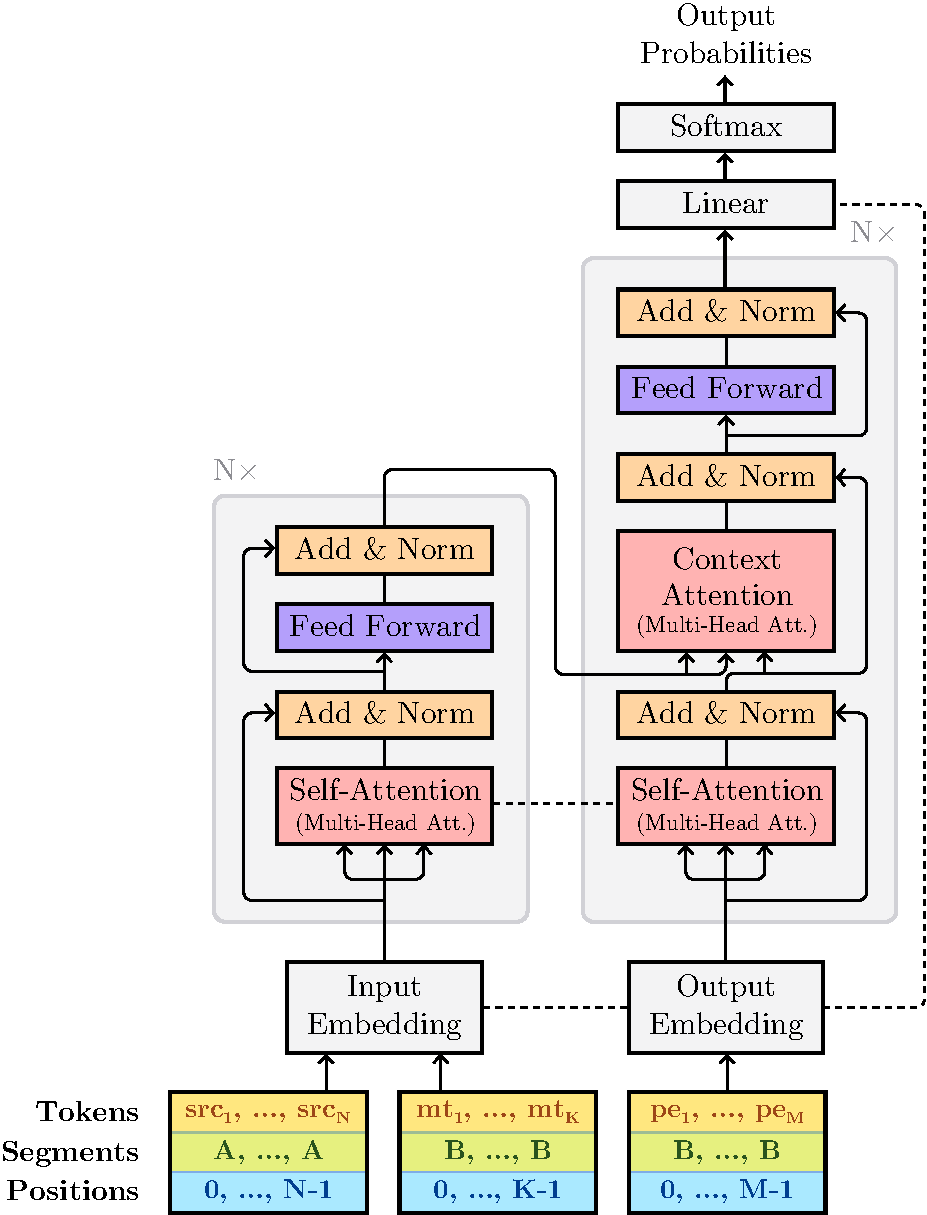
\includegraphics[width=0.9\textwidth]{Figures/bert-ape-diagram.pdf}
    \caption[Dual-Source BERT.]{Dual-Source BERT. Dashed lines show which blocks have shared parameters in our best configuration.}
    \label{fig:transformer_diagram}
\end{figure}

\section{Automatic Post-Editing with BERT}\label{sec:ape_bert}

\subsection{BERT as a Cross-Lingual Encoder}

\noindent Our transfer learning approach is based on the Bidirectional Encoder
Representations from Transformers~\citep[BERT;][]{devlin2018bert}.
This model obtains deep bidirectional representations by training a
transformer~\citep{vaswani2017attention} with a large-scale dataset
in a masked language modeling task where the objective is to predict
missing words in a sentence. In our experiments, we use the BERT\textsubscript{BASE}
model, which is composed of $N\!\!=\!\!12$ self-attention layers, hidden size
$K\!\!=\!768$, $H\!\!=\!\!12$ attention heads, and feed-forward inner layer size
$F\!\!=\!3072$. In addition to the word and learned position embeddings,
BERT also has {\bf segment embeddings} to differentiate between a
segment A and a segment B\,---\,this is useful for tasks such as natural
language inference, which involves two sentences. In the case of APE,
there is also a pair of input sentences ({\tt src}, {\tt mt}) which
are in different languages. Since one of the released BERT models was
jointly pre-trained on 104 languages,\footnote{
    \url{https://github.com/google-research/bert/blob/eedf5716ce1268e56f0a50264a88cafad334ac61/multilingual.md}}
we use this multilingual BERT pre-trained model to encode the
bilingual input pair of APE.

Therefore, the whole encoder of our APE model is the multilingual
BERT: we encode both {\tt src} and {\tt mt} in the same encoder and
use the segment embeddings to differentiate between languages
(\figref{fig:transformer_diagram}). We reset positional
embeddings when the {\tt mt} starts, since it is not a continuation
of {\tt src}.

\subsection{BERT as a Decoder}\label{sec:ape_bert_decoder}

\noindent Prior work has incorporated pre-trained models as {\it encoders}, but
not as {\bf decoders} of sequence-to-sequence models. Doing so
requires a strategy for generating fluently from the pre-trained
model. Note that, when using BERT as a decoder, its bidirectionality is lost, since the
model cannot look at words that have not been generated yet, and it
is an open question of how to learn decoder-specific blocks (\eg,
context attention), which are absent in the pre-trained model.

One of our key contributions is to use BERT in the decoder by
experimenting with different strategies for initializing and sharing the
self and context attention layers and the position-wise feed-forward
layers. We tie together the encoder and decoder embeddings weights
(word, position, and segment) along with the decoder output layer
(transpose of the word embedding layer). We use the same segment
embedding for the target sentence ({\tt pe}) and the second sentence
in the encoder ({\tt mt}) since they are in the same language. The
full architecture is shown in \figref{fig:transformer_diagram}.

We experiment with the following strategies for coupling BERT
pre-trained models in the decoder:
%
\begin{itemize}
    \item \textbf{Transformer.} A transformer decoder as described in
          \citet{vaswani2017attention} without any shared parameters,
          with the same dimensions as BERT\textsubscript{BASE} but with randomly
          initialized weights.
    \item \textbf{Pre-trained BERT.} This initializes the decoder with
          the pre-trained BERT model. The only component initialized randomly
          is the context attention (CA) layer, which is absent in BERT. Unlike
          in the original BERT model\,---\,which only encodes sentences\,---\,a mask in
          the self-attention is required to prevent the model from looking to
          subsequent tokens in the target sentence.
    \item \textbf{ BERT initialized context attention.} Instead of a
          random initialization, we initialize the context attention layers
          with the weights of the corresponding BERT self-attention layers.
    \item \textbf{Shared self-attention}. Instead of just having the same
          initialization, the self-attentions (SA) in the encoder and decoder
          are tied during training.
    \item \textbf{Context attention shared with self-attention.} We take
          a step further and \emph{tie} the context attention and self-attention
          weights\,---\,making all the attention transformation matrices
          (self and context) in the encoder and decoder tied.
    \item \textbf{Shared feed-forward.} We tie the feed-forward weights
          (FF) between the encoder and decoder.
\end{itemize}

\section{Experiments} \label{sec:experiments}

\noindent We now describe our experimental results. Our models were implemented
on a fork of OpenNMT-py~\citep{klein2017opennmt} using HuggingFace's
transformers
library.\footnote{\url{https://github.com/huggingface/transformers}}
Our model's implementation is publicly
available.\footnote{\url{https://github.com/deep-spin/OpenNMT-APE}}

\paragraph*{Datasets.}
We use the data from the WMT 2018 APE shared
task~\citep{Chatterjee2018} (English-German SMT), which consists of
23K triplets for training, 1K for validation, and 2K for
testing. In some experiments, we use the eSCAPE
corpus~\citep{negri2018escape}, which comprises about 8M sentences;
when doing so, we oversample 35x the shared task data to cover $10\%$
of the training data. We segment words with
WordPiece~\citep{wu2016google}, as used in the
Multilingual BERT. At training time, we discard triplets with 200+
tokens in the combination of {\tt src} and {\tt mt} or 100+ tokens in
    {\tt pe}. For evaluation, we use TER~\citep{snover2006study} and
tokenized BLEU~\citep{papineni2002bleu}.

\paragraph*{Training Details.}
We use Adam~\citep{kingma2014adam} with a triangular learning rate
schedule that increases linearly during the first 5,000 steps until
$5\times 10^{-5}$ and has a linear decay afterward. When using BERT
components, we use a $\ell_2$ weight decay of $0.01$. We apply
dropout~\citep{srivastava2014dropout} with $p_{\text{drop}}\!=\!0.1$ to all
layers and use label smoothing with
$\epsilon\!=\!0.1$~\citep{pereyra2017regularizing}. For the small data
experiments, we use a batch size of 1024 tokens and save checkpoints
every 1,000 steps; when using the eSCAPE corpus, we increase this to
2048 tokens and 10,000 steps. The checkpoints are created with the
exponential moving average strategy of \citet{junczys2018marian}
with a decay of $10^{-4}$. At test time, we select the model with
the best TER on the development set and apply beam search with a beam
size of 8 and using an average length penalty.

\begin{table}[t]
    \centering
    \tlfstyle
    \begin{tabular}{lcc}
        \toprule
                                                           & TER$\downarrow$ & BLEU$\uparrow$ \\
        \midrule
        Transformer decoder                                & 20.33           & 69.31          \\
        Pre-trained BERT                                   & 20.83           & 69.11          \\
        \hspace{1ex}\textcolor{gray}{\textit{with}}
        CA $\leftarrow$ SA                                 & 18.91           & 71.81          \\
        \textover[r]
        {\hspace{1ex}\textcolor{gray}{\textit{and}}}{\hspace{1ex}\textit{with}}
        \textover[r]
        {SA $\leftrightarrow$}
        {CA $\leftarrow$} Encoder SA                       & \textbf{18.44}  & \textbf{72.25} \\
        \textover[r]
        {\hspace{1ex}\textcolor{gray}{\textit{and}}}{\hspace{1ex}\textit{with}}
        \textover[r]
        {CA $\leftrightarrow$}{CA $\leftarrow$} SA         & 18.75           & 71.83          \\
        \textover[r]
        {\hspace{1ex}\textcolor{gray}{\textit{and}}}{\hspace{1ex}\textit{with}}
        \textover[r]
        {FF $\leftrightarrow$}{CA $\leftarrow$} Encoder FF & 19.04           & 71.53          \\
        \bottomrule
    \end{tabular}
    \caption[Ablation study of decoder configurations.]{
        Ablation study of decoder configurations, by gradually having more
        shared parameters between the encoder and decoder (trained without
        synthetic data). $\leftrightarrow$ denotes parameter tying and
        $\leftarrow$ an initialization.
    }
    \label{tab:ablation_smt}
\end{table}

\begin{landscape}
    \begin{table*}[t]
        \centering
        \tlfstyle
        \begin{tabular}{lccccccc}
            \toprule
                                                             &                & \multicolumn{2}{c}{test 2016} &
            \multicolumn{2}{c}{test 2017}                    &
            \multicolumn{2}{c}{test 2018}                                                                                                      \\
            \cmidrule{3-4} \cmidrule{5-6}  \cmidrule{7-8}
            Model                                            & Train Size     & TER$\downarrow$               & BLEU$\uparrow$ &
            TER$\downarrow$                                  & BLEU$\uparrow$ & TER$\downarrow$               & BLEU$\uparrow$                 \\
            \midrule
            MT baseline (Uncorrected)                        &                &
            24.76                                            & 62.11          & 24.48                         & 62.49          & 24.24 & 62.99 \\
            \midrule
            \citet{berard2017lig}                            &
            \multicolumn{1}{c}{23K}                          &
            22.89                                            & ---            & 23.08                         & 65.57          & ---   & ---   \\
            \midrule
            \citet{junczys2018ms}                            &
            \multicolumn{1}{c}{\multirow{2}{*}{5M}}          &
            18.92                                            & 70.86          & 19.49                         & 69.72          & ---   & ---   \\
            \citet{junczys2018ms}$\times 4$                  &
            \multicolumn{1}{c}{}                             &
            18.86                                            & 71.04          & 19.03                         & 70.46          & ---   & ---   \\
            \midrule
            \citet{tebbifakhr2018multi}                      &
            \multicolumn{1}{c}{\multirow{3}{*}{8M}}          &
            ---                                              & ---            & ---                           & ---            & 18.62 & 71.04 \\
            \citet{junczys2018ms}                            &
            \multicolumn{1}{c}{}                             &
            17.81                                            & 72.79          & 18.10                         & 71.72          & ---   & ---   \\
            \citet{junczys2018ms}$\times 4$                  &
            \multicolumn{1}{c}{}                             &
            17.34                                            & 73.43          & 17.47                         & 72.84          & 18.00 & 72.52 \\
            \midrule
            \midrule
            Dual-Source Transformer$^\dagger$                &
            \multicolumn{1}{c}{\multirow{4}{*}{23K}}         &
            27.80                                            & 60.76          & 27.73                         & 59.78          & 28.00 & 59.98 \\
            BERT Enc.\,+\,Transformer Dec. (\emph{Ours})     &
            \multicolumn{1}{c}{}                             &
            20.23                                            & 68.98          & 21.02                         & 67.47          & 20.93 & 67.60 \\
            BERT Enc.\,+\,BERT Dec. (\emph{Ours})            &
            \multicolumn{1}{c}{}                             &
            18.88                                            & 71.61          & 19.03                         & 70.66          & 19.34 & 70.41 \\
            BERT Enc.\,+\,BERT Dec. $\times 4$ (\emph{Ours}) &
            \multicolumn{1}{c}{}                             &
            \textbf{18.05}                                   & \textbf{72.39} & \textbf{18.07}                &
            \textbf{71.90}                                   & \textbf{18.91} & \textbf{70.94}                                                 \\
            \midrule
            BERT Enc.\,+\,BERT Dec. (\emph{Ours})            &
            \multicolumn{1}{c}{\multirow{2}{*}{8M}}          &
            16.91                                            & 74.29          & 17.26                         & 73.42          & 17.71 & 72.74 \\
            BERT Enc.\,+\,BERT Dec. $\times 4$ (\emph{Ours}) &
            \multicolumn{1}{c}{}                             &
            \textbf{16.49}                                   & \textbf{74.98} & \textbf{16.83}                &
            \textbf{73.94}                                   & \textbf{17.15} & \textbf{73.60}                                                 \\
            \bottomrule
        \end{tabular}
        \caption[Results on the WMT 2016--18 APE shared task datasets.]{
            Results on the WMT 2016--18 APE shared task datasets. Our
            single models trained on the 23K dataset took only 3h20m to converge
            on a single Nvidia GeForce GTX 1080 GPU, while results for models
            trained on 8M triplets take approximately 2 days on the same GPU.
            Models marked with ``$\times 4$'' are ensembles of 4 models.
            Dual-Source Transformer$^\dagger$ is a comparable re-implementation
            of \citet{junczys2018ms}. Best results for each training size (23K and 8M) are shown in \textbf{bold}.}
        \label{tab:results_smt}
    \end{table*}
\end{landscape}

\paragraph*{Initialization and Parameter Sharing.}
\tableref{tab:ablation_smt} compares the different decoder
strategies described in \secref{sec:ape_bert_decoder} on the WMT 2018
validation set. The best results were achieved by sharing the
self-attention between encoder and decoder, and by initializing (but
not sharing) the context attention with the same weights as the
self-attention. Regarding the self-attention sharing, we hypothesize
that its benefits are due to both encoder and decoder sharing a
common language in their input (in the {\tt mt} and {\tt pe}
sentence, respectively). Future work will investigate if this is
still beneficial when the source and target languages are less
similar. On the other hand, the initialization of the context
attention with BERT's self-attention weights is essential to reap the
benefits of BERT representations in the decoder\,---\,without it, using
BERT decreases performance when compared to a regular transformer
decoder. This might be because context attention and
self-attention share the same neural block architecture (multi-head
attention) and thus the context attention benefits from the
pre-trained BERT's better weight initialization. No benefit was
observed from sharing the feed-forward weights.

\paragraph*{Final Results and Analysis.}
Finally, \tableref{tab:results_smt} shows our results on the WMT
2016--18 test sets. The model named \emph{BERT Enc.\,+\,BERT Dec.}
corresponds to the best setting found in
\tableref{tab:ablation_smt}, while \emph{BERT Enc.\,+\,Transformer
    Dec.} only uses BERT in the encoder. We show results for single
models and ensembles of 4 independent models.

Using the small shared task dataset only (23K triplets), our single
\emph{BERT Enc.\,+\,BERT Dec.} model surpasses the MT baseline by a
large margin ($-$4.90 TER in test 2018). The only system we are aware
to beat the MT baseline with only the shared task data is
\citet{berard2017lig}, which we also outperform ($-$4.05 TER in test
2017). With only about 3 GPU hours and on a much smaller dataset, our
model reaches a performance that is comparable to an ensemble of the
best WMT 2018 system with an artificial dataset of 5M triplets
($+$0.02 TER in test 2016), which is much more expensive to train.
With 4$\times$ ensembling, we get competitive results with systems
trained on 8M triplets.

When adding the eSCAPE corpus (8M triplets), performance surpasses
the state of the art in all test sets. By ensembling, we improve even
further, achieving a final 17.15 TER score in test 2018 ($-$0.85 TER
than the previous state of the art).

\section{Subsequent Work}

\noindent After our publication~\citep{Correia2019}, many works have since been
published exploring the use of large pre-trained language models for
generation purposes (\eg,
\citep{zhang2019PretrainingBasedNaturalLanguage,
    chen2020DistillingKnowledgeLearned}), and our work shown in this
chapter was one of the first to do so.

Most closely related to our work, and co-authored by the writer of
the present thesis, \citet{Lopes2019} used our model on the
harder English-German NMT APE subtask of WMT 2019, winning the shared
task that year. To obtain this result, the transfer learning
capabilities of BERT were not enough and further engineering effort
was required. Particularly, a conservativeness factor was added
during beam decoding to constrain the changes the APE system can make
to the {\tt mt} output. Furthermore, the authors used a data
weighting method to augment the importance of data samples that have
lower TER. By doing this, data samples that required less
post-editing effort are assigned higher weights during the training
loop. Since the NMT system does very few errors on this domain this
data weighting is important for the APE model to learn to do fewer
corrections to the {\tt mt} output. However, their approach required
the creation of an artificial dataset to obtain a performance that
improved the MT baseline. Further investigation is required in APE to
come up with better methods that obtain improved results compared to
the baseline using only real post-edited data in these smaller APE
datasets based on NMT outputs rather than SMT ones.

In the following years of the APE subtask, we have seen models that
have been inspired by our BERT model. Particularly,
\citet{lee2020POSTECHETRISubmissionWMT2020} used an
XLM~\citep{lample2019xlm} inspired model in the 2020 APE WMT subtask,
instead of the multilingual BERT that our work used. Another
submission to that year's subtask pre-trained their own BERT-like
model on a cross-lingual dataset, making it predict the target
language during this pre-training
stage~\citep{wang2020AlibabaSubmissionWMT}.

On the data-efficiency side,
\citet{gois2020LearningNonMonotonicAutomatic} performed
experiments on the APE subtask, using only the real post-edited data,
without recurring to expensive synthetic dataset creation. In their
case, they also leveraged transfer learning using a BERT encoder, but
increased the decoder's supervision to include real keystrokes data,
from human post-editors. While not surpassing our approach, we
consider this to also be a promising direction: increasing inductive
bias in an effort to decrease larger data dependency. To address the
more difficult challenge of doing APE on NMT outputs,
\citet{chollampatt2020CanAutomaticPostEditing} used our model to
explore how many training instances are needed to achieve a better
performance than the harder \emph{do-nothing} NMT baseline and have
concluded that, while substantial improvements for NMT require more
data samples than SMT, the APE model can still improve upon the
baseline with relatively few instances. To improve future
APE research, they have released a more appropriately-sized dataset
of real post-edited NMT data of 161K training instances based on
subtitles (\emph{SubEdits}).

The approach conducted in this chapter has also been successfully
generalized to other tasks. \citet{kodama2020GeneratingResponsesthat}
used our model for the generation of responses of a dialogue system,
where, in the input, instead of \texttt{src} and a tentative
\texttt{mt} output, they concatenate a question with meta-data that
indicates how the system should generate a response in terms of
emotion and intimacy. As in our APE case, they also achieve good
performance on a low-resource dataset. Even more generally,
\citet{huang2021TransferLearningSequence} identifies APE as a part of
a family of generation tasks in which there are multiple inputs.
Inspired by our approach, they also tackle the low-resource nature of
these tasks by leveraging weak supervision through transfer learning.
To mitigate catastrophic forgetting, they propose a \emph{gradual
    fine-tuning} approach, in which they do an additional fine-tuning
stage to adapt the pre-trained language model to a single-source
sequence-to-sequence task, before finally fine-tuning on the
multiple-source sequence-to-sequence task. They achieve increased
performance on low-resource datasets, not only for APE but also for
multi-source translation and document-level translation.

\section{Final Remarks and Chapter Summary}

\noindent In this chapter, we proposed a transfer learning approach to APE
using BERT pre-trained models and careful parameter sharing. We
explored various ways of coupling BERT in the decoder for language
generation. We found it beneficial to initialize the context
attention of the decoder with BERT's self-attention and to tie
together the parameters of the self-attention layers between the
encoder and decoder. Using a small dataset, our results are
competitive with systems trained on a large amount of artificial
data, with much faster training. By adding artificial data, we obtain
a new state of the art in APE. We hope that our approach will
continue to inspire future work in leveraging weak supervision
through transfer learning to improve performance on generation tasks
that have scarce real data.

\cleardoublepage

\singlespacing
\fancychapter[Adaptively Sparse Transformers]{Adaptively Sparse Transformers}
\label{chap:adaptsparse}

\cleardoublepage
\doublespacing

\noindent In the previous chapter, we used transfer learning as a way
to weakly supervise a transformer model on a low-resource task.
While we achieved good results with this approach, the
architecture of the transformer remains largely uninterpretable,
which is unappealing if one wishes to find the
reasons behind the strengths and shortcomings of the model.

To this end, we introduce in the present chapter an approach that
uses \textbf{learnable sparsity} on each of the transformer's
attention heads. In the context of this thesis, this contribution
leads to neural models that are more \textbf{transparent} in their
decisions. This increased transparency will prove useful in order to
be able to more easily interpret the roles that each attention head
ends up playing in the overall model.

\textit{This chapter is based on \citet*{correia2019adaptively}.}

\section{Motivation}

\noindent At the heart of the transformer architecture
(\secref{sec:transformer_bg}) lie \emph{multi-head attention}
mechanisms: each word is represented by multiple different weighted
averages of its relevant context. As suggested by recent works on
interpreting attention head roles, separate heads may learn
to look for various relationships between
tokens~\citep{tang2018why,raganato2018analysis,
    marecek-rosa-2018-extracting,bert-rediscovers,specialized}.

The attention distribution of each head in the transformer is
predicted typically using the \textbf{softmax} normalizing transformation.
As a result, all context words have non-zero attention weight. Recent
work on single attention architectures suggests that using sparse
normalizing transformations in attention mechanisms such as sparsemax --
which can yield exactly zero probabilities for irrelevant words --
may improve performance and
interpretability~\citep{malaviya2018sparse,deng2018latent,entmax}.
Qualitative analysis of attention heads
\citep[Figure~5]{vaswani2017attention} suggests that, depending on
what phenomena they capture, heads tend to favor flatter or more
peaked distributions.

Recent works have proposed Sparse
Transformers~\citep{openai_sparse_transf} and Adaptive Span
Transformers~\citep{Sukhbaatar2019}. However, the ``sparsity" of those
models only limits the attention to a contiguous span of past tokens,
while in this work we propose a \textbf{highly adaptive} transformer
model that is capable of attending to a sparse set of words that are
not necessarily contiguous. \figref{fig:comparison} shows the
relationship of these methods with ours.

Our contributions are the following:

\begin{itemize}
    \item We introduce \textbf{sparse attention} into the
          transformer architecture, showing that it eases
          interpretability and leads to slight accuracy gains.
    \item We propose an adaptive version of sparse attention,
          where the shape of each attention head is {\bf learnable} and can vary continuously and
          dynamically between the dense limit case of \emph{softmax} and the sparse,
          piecewise-linear \emph{sparsemax} case.\footnote{
              Code and pip package available at \url{https://github.com/deep-spin/entmax}.}
    \item We make an extensive analysis of the added interpretability of these
          models, identifying both crisper examples of attention head behavior observed in
          previous work, as well as novel behaviors unraveled thanks to the sparsity
          and adaptivity of our proposed model.
\end{itemize}

\begin{figure}[htbp]
    \centering
    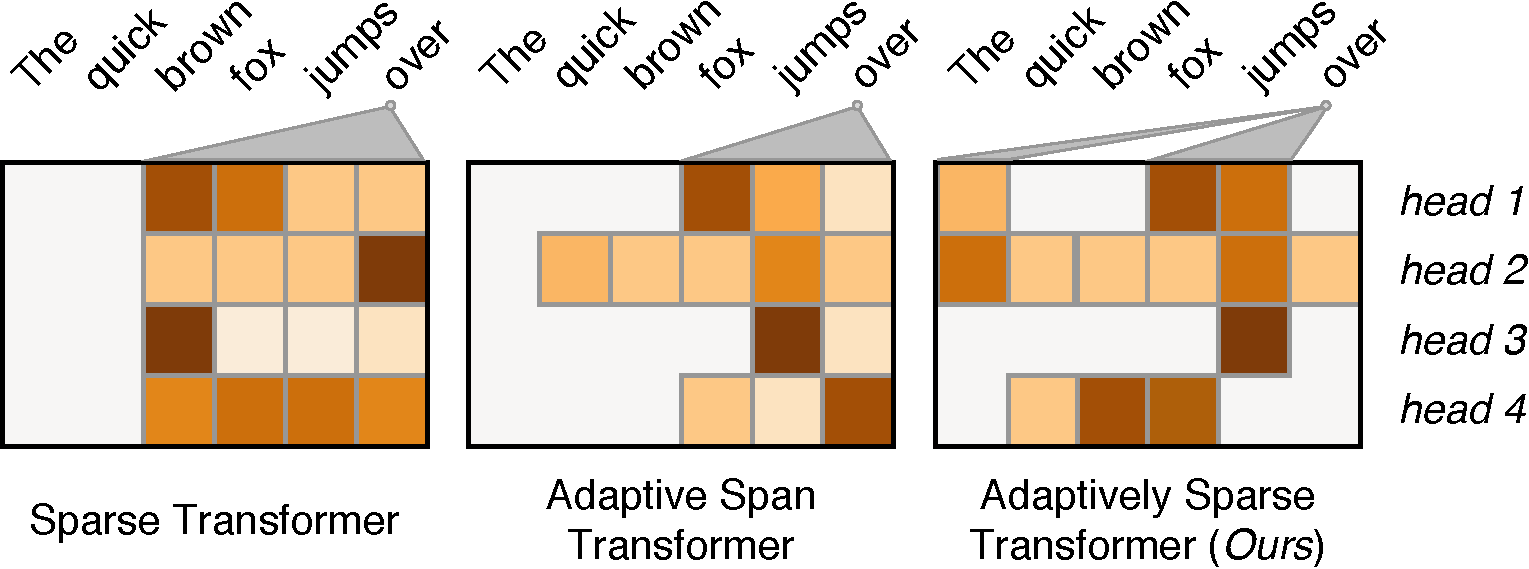
\includegraphics[width=0.95\columnwidth]{Figures/comparison.pdf}
    \caption{Attention distributions of different self-attention heads for the
        time step of the token ``over'', shown to compare our model to other
        related work. While the Sparse
        Transformer~\citep{openai_sparse_transf} and the Adaptive Span
        Transformer~\citep{Sukhbaatar2019} only attend to words within a
        contiguous span of the past tokens, our model is not only able to
        obtain different and not necessarily contiguous sparsity patterns for
        each attention head, but is also able to tune its support over which
        tokens to attend adaptively.}
    \label{fig:comparison}
\end{figure}

\section{Previous Work}

\paragraph*{Sparse attention.}
Prior work has developed sparse attention mechanisms, including
applications to NMT~\citep{sparsemax, malaviya2018sparse, fusedmax,
    shao2019ssn, maruf2019selective}. \citet{entmax} introduced the
\entmaxtext function this work builds upon. In their work, there is a
single attention mechanism which is controlled by a fixed $\alpha$.
In contrast, this is the first work to allow such attention mappings
to \emph{dynamically} adapt their curvature and sparsity, by
automatically adjusting the continuous $\alpha$ parameter. We also
provide the first results using sparse attention in a transformer
model.

\paragraph*{Fixed sparsity patterns.}
Recent research improves the scalability of transformer-like networks
through static, fixed sparsity patterns
\citep{openai_sparse_transf,dynamic_conv}. Our adaptively-sparse
transformer can dynamically select a sparsity pattern that finds
relevant words regardless of their position (\eg,
\figref{fig:head_interro}). Moreover, the two strategies could be
combined. In a concurrent line of research, \citet{Sukhbaatar2019}
propose an adaptive attention span for transformer language models.
While their work has each head learn a different contiguous span of
context tokens to attend to, our work finds different sparsity
patterns in the same span. Interestingly, some of their findings
mirror ours---we found that attention heads in the last layers tend
to be denser on average when compared to the ones in the first
layers, while their work has found that lower layers tend to have a
shorter attention span than higher layers.

\paragraph*{Transformer interpretability.} The original transformer
paper~\citep{vaswani2017attention} shows attention visualizations,
from which some speculation can be made of the roles the several
attention heads have. \citet{marecek-rosa-2018-extracting} study the
syntactic abilities of the transformer self-attention, while
\citet{raganato2018analysis} extract dependency relations from the
attention weights. \citet{bert-rediscovers} find that the
self-attentions in BERT~\citep{devlin2018bert} follow a sequence of
processes that resembles a classical NLP pipeline. Regarding
redundancy of heads, \citet{specialized} develop a method that is
able to prune heads of the multi-head attention module and make an
empirical study of the role that each head has in self-attention
(positional, syntactic and rare words). \citet{li2018multi} also aim
to reduce head redundancy by adding a regularization term to the loss
that maximizes head disagreement and obtain improved results. While
not considering transformer attentions, \citet{jain2019attention}
show that traditional attention mechanisms do not necessarily improve
interpretability since softmax attention is vulnerable to an
adversarial attack leading to wildly different model predictions for
the same attention weights. Sparse attention may mitigate these
issues; however, our work focuses mostly on a more mechanical aspect
of interpretation by analyzing head behavior, rather than on
explanations for predictions.

\section{Adaptively Sparse Transformers}
\label{sec:adaptive}

\noindent We now propose a novel transformer architecture wherein we simply replace
softmax with $\alpha$-\entmaxtext{}, described in
\secref{sec:entmax_bg}, in the attention heads. Concretely, we
replace the row normalization $\amap$ in \eqnref{eq:att_scaled_dot}
by
%
\begin{equation}
    \amap(\bm{Z})_{ij} = \aentmax(\bm{z}_i)_j.
\end{equation}
%
This change leads to sparse attention weights, as long as
$\alpha>1$; in particular, $\alpha=1.5$ is a sensible starting
point~\citep{entmax}.

\paragraph*{Different {\boldmath $\alpha$} per head.}
Unlike LSTM-based seq2seq models, where $\alpha$ can be more easily
tuned by grid search, in a transformer, there are many attention
heads in multiple layers. Crucial to the power of such models, the
different heads capture different linguistic phenomena, some of them
isolating important words, others spreading out attention across
phrases~\citep[Figure~5]{vaswani2017attention}. This motivates using
different, adaptive $\alpha$ values for each attention head, such
that some heads may learn to be sparser, and others may become closer
to softmax. We propose doing so by treating the $\alpha$ values as
neural network parameters, optimized via stochastic gradients along
with the other weights.

\paragraph*{Derivatives \wrt~{\boldmath $\alpha$}.}
In order to optimize $\alpha$ automatically via gradient methods, we
must compute the Jacobian of the \entmaxtext output \wrt $\alpha$.
Since \entmaxtext is defined through an optimization problem, this is
non-trivial and cannot be simply handled through automatic
differentiation; it falls within the domain of \emph{argmin
    differentiation}, an active research topic in optimization
\citep{gould,optnet}.

One of our key contributions is the derivation of a closed-form
expression for this Jacobian. The next proposition provides
such an expression, enabling \entmaxtext layers with
adaptive $\alpha$. To the best of our knowledge, ours is the first
neural network module that can automatically, continuously vary in
shape away from softmax and toward sparse mappings like sparsemax.

\begin{proposition}\label{prop:grad_alpha}%
    Let $\p^\star \coloneqq \aentmax(\x)$ be the solution of
    \eqnref{eq:define_entmax}.
    Denote the distribution $\tilde{\pp}_i \coloneqq \nicefrac{(\pp_i^\star)^{2 - \alpha}}{
            \sum_j(\pp_j^\star)^{2-\alpha}}$ and let
    $h_i \coloneqq -\pp^\star_i \log \pp^\star_i$.
    The $i$\textsuperscript{th} component of the Jacobian
    $\bm{g} \coloneqq \pfrac{\aentmax(\x)}{\alpha}$ is
    \begin{equation}\label{eq:final_gradient_alpha}
        g_i =%
        \begin{cases}
            \frac{p_i^{\star} - \tilde{\pp}_i}{(\alpha-1)^2} +
            \frac{h_i - \tilde{\pp}_i%
                \sum_j h_j%
            }{\alpha-1},                                                                  & \alpha > 1, \\[1.5ex]
            \frac{h_i \log \pp_i^{\star} - \pp_i^{\star} \sum_j h_j \log p_j^{\star}}{2}, & \alpha = 1.
        \end{cases}
    \end{equation}
\end{proposition}
\noindent%
The proof uses implicit function differentiation and is given in \appref{app:alpha_grad}.

\eqnref{eq:final_gradient_alpha} provides the remaining missing
piece needed for training adaptively sparse transformers. In the
following section, we evaluate this strategy on neural machine
translation, and analyze the behavior of the learned attention heads.

\section{Experiments}

\noindent We apply our adaptively sparse transformers on four MT tasks.
For comparison, a natural baseline is the standard transformer
architecture using the softmax transform in its multi-head attention mechanisms.
We consider two other model variants in our experiments that make use of different
normalizing transformations:

\begin{itemize}
    \item \textbf{1.5-\entmaxtext:} a transformer with sparse \entmaxtext
          attention with fixed $\alpha=1.5$ for all heads. This is a novel model,
          since 1.5-\entmaxtext{} had only been used on
          RNN-based NMT models~\citep{entmax}, but never
          in transformers, where attention modules are not just one single
          component of the model but rather an integral part of all of
          the model components.%
    \item \textbf{\boldmath $\alpha$-\entmaxtext:} an \textbf{adaptive}
          transformer with sparse \entmaxtext attention with a different,
          learned $\alpha_{i,j}^t$ for each head.
\end{itemize}

The adaptive model has an additional scalar parameter per attention
head for each of the three attention mechanisms (encoder
self-attention, context attention, and decoder self-attention), \ie,
\begin{equation}
    \big \{ a_{i,j}^{t} \in \reals:~
    i \in \{1, \dots, L\},~
    j \in \{1, \dots, H\},~
    t \in \{\texttt{enc}, \texttt{ctx}, \texttt{dec}\} \big\},
\end{equation}
and we set $\alpha_{i,j}^t = 1 + \sigmoid(a_{i,j}^t) \in ]1, 2[$.
All or some of the $\alpha$ values can be tied if desired, but we
keep them independent for analysis purposes.

\paragraph*{Datasets.} Our models were trained on 4 machine
translation datasets of different number of training instances
(sentence pairs):

\begin{itemize}[itemsep=.5ex,leftmargin=2ex]
    \item IWSLT 2017 German$\rightarrow$English
          \citep[\langp{de}{en},][]{cettolooverview}: ~200K.
    \item KFTT Japanese$\rightarrow$English
          \citep[\langp{ja}{en},][]{neubig11kftt}: ~300K.
    \item WMT 2016 Romanian$\rightarrow$English
          \citep[\langp{ro}{en},][]{bojar2016findings}: ~600K.
    \item WMT 2014 English$\rightarrow$German
          \citep[\langp{en}{de},][]{bojar2014findings}: ~4.5M.
\end{itemize}

All of these datasets were preprocessed with byte-pair
encoding~\citep[BPE;][]{sennrich2016neural}, using joint
segmentations of 32K merge operations.

\paragraph*{Training.}
We follow the dimensions of the Transformer-Base model of
\citet{vaswani2017attention}: The number of layers is $L=6$ and
number of heads is $H=8$ in the encoder self-attention, the context
attention, and the decoder self-attention. We use a mini-batch size
of 8192 tokens and warm up the learning rate linearly until 20k
steps, after which it decays according to an inverse square root
schedule. All models were trained until convergence of validation
accuracy, and evaluation was done at each 10K steps for
\langp{ro}{en} and \langp{en}{de} and at each 5K steps for
\langp{de}{en} and \langp{ja}{en}. The end-to-end computational
overhead of our methods, when compared to standard softmax, is
relatively small; in training tokens per second, the models using
$\alpha$-\entmaxtext and $1.5$-\entmaxtext are, respectively, $75\%$
and $90\%$ the speed of the softmax model.

\paragraph*{Results.}
We report test set tokenized BLEU~\citep{papineni2002bleu} results in
\tableref{table:mt}. We can see that replacing softmax by
\entmaxtext{} does not hurt performance in any of the datasets;
indeed, sparse attention transformers tend to have slightly higher
BLEU, but their sparsity leads to a better potential for analysis. In
the next section, we make use of this potential by exploring the
learned internal mechanics of the self-attention heads.

\begin{table*}[ht]
    \begin{center}
        \tlfstyle
        \begin{tabular}{lrrrr}
            \toprule
            activation
             & \langp{de}{en} & \langp{ja}{en}
             & \langp{ro}{en} & \langp{en}{de} \\
            \midrule
            $\softmax$
             & 29.79
             & 21.57
             & 32.70
             & 26.02                           \\
            $\aentmax[1.5]$
             & 29.83
             & \textbf{22.13}
             & \textbf{33.10}
             & 25.89                           \\
            $\aentmax[\alpha]$
             & \textbf{29.90}
             & 21.74
             & 32.89
             & \textbf{26.93}                  \\
            \bottomrule
        \end{tabular}
    \end{center}
    \caption{Machine translation tokenized BLEU test results
        on IWSLT 2017 \langp{de}{en},
        KFTT \langp{ja}{en}, WMT 2016 \langp{ro}{en} and
        WMT 2014 \langp{en}{de}, respectively.\label{table:mt}}
\end{table*}

\section{Analysis}

\noindent We conduct high-level analysis of the learned attention heads of the
sparse adaptive transformer model ($\alpha$-\entmaxtext) trained on
the 4 datasets. We then present, for the higher-resource dataset WMT
2014 English $\rightarrow$ German, a more detailed analysis of the
attention at the individual head behavior. Moreover, we make a
qualitative analysis of the interpretability capabilities of our
models.

\subsection{High-Level Statistics}
\label{sec:stats}

\begin{figure}[ht]
    \centering
    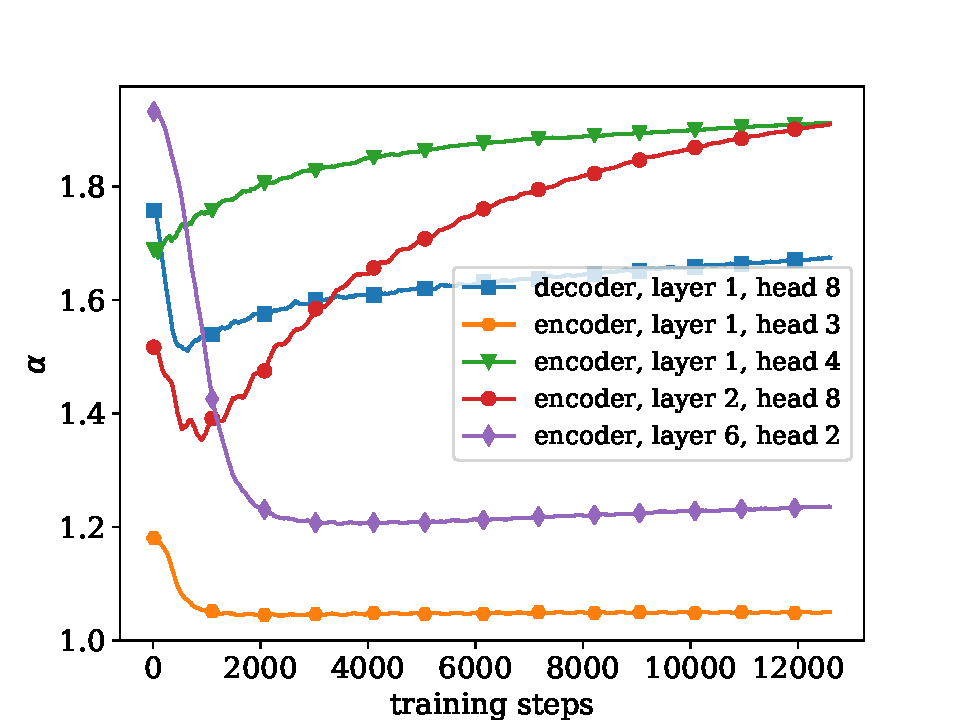
\includegraphics[width=0.95\columnwidth]{Figures/learning_alpha.pdf}
    \caption{\label{fig:learning_alpha}
        Trajectories of $\alpha$ values for a subset of the heads during
        training. Initialized at random, most heads become denser in the
        beginning, before converging. This suggests that dense attention may
        be more beneficial while the network is still uncertain, being
        replaced by sparse attention afterwards.}
\end{figure}

\paragraph*{What kind of {\boldmath $\alpha$} values are learned?}
\figref{fig:learning_alpha} shows the learning trajectories of the
$\alpha$ parameters of a selected subset of heads. We generally
observe a tendency for the randomly-initialized $\alpha$ parameters
to decrease initially, suggesting that softmax-like behavior may be
preferable while the model is still uncertain. After around one
thousand steps, some heads change direction and become sparser,
perhaps as they become more confident and specialized. This shows
that the initialization of $\alpha$ does not predetermine its
sparsity level or the role the head will have throughout. In
particular, head $8$ in the encoder self-attention layer $2$ first
drops to around $\alpha=1.3$ before becoming one of the sparsest
heads, with $\alpha\approx2$.

The overall distribution of $\alpha$ values at convergence can be
seen in \figref{fig:hist_alphas}. We can observe that the encoder
self-attention blocks learn to concentrate the $\alpha$ values in two
modes: a very sparse one around $\alpha \rightarrow 2$, and a dense
one between softmax and 1.5-\entmaxtext{}. However, the decoder self
and context attention only learn to distribute these parameters in a
single mode. We show next that this is reflected in the average
density of attention weight vectors as well.

\begin{figure}[!htbp]
    \centering
    \begin{subfigure}[b]{.49\linewidth}
        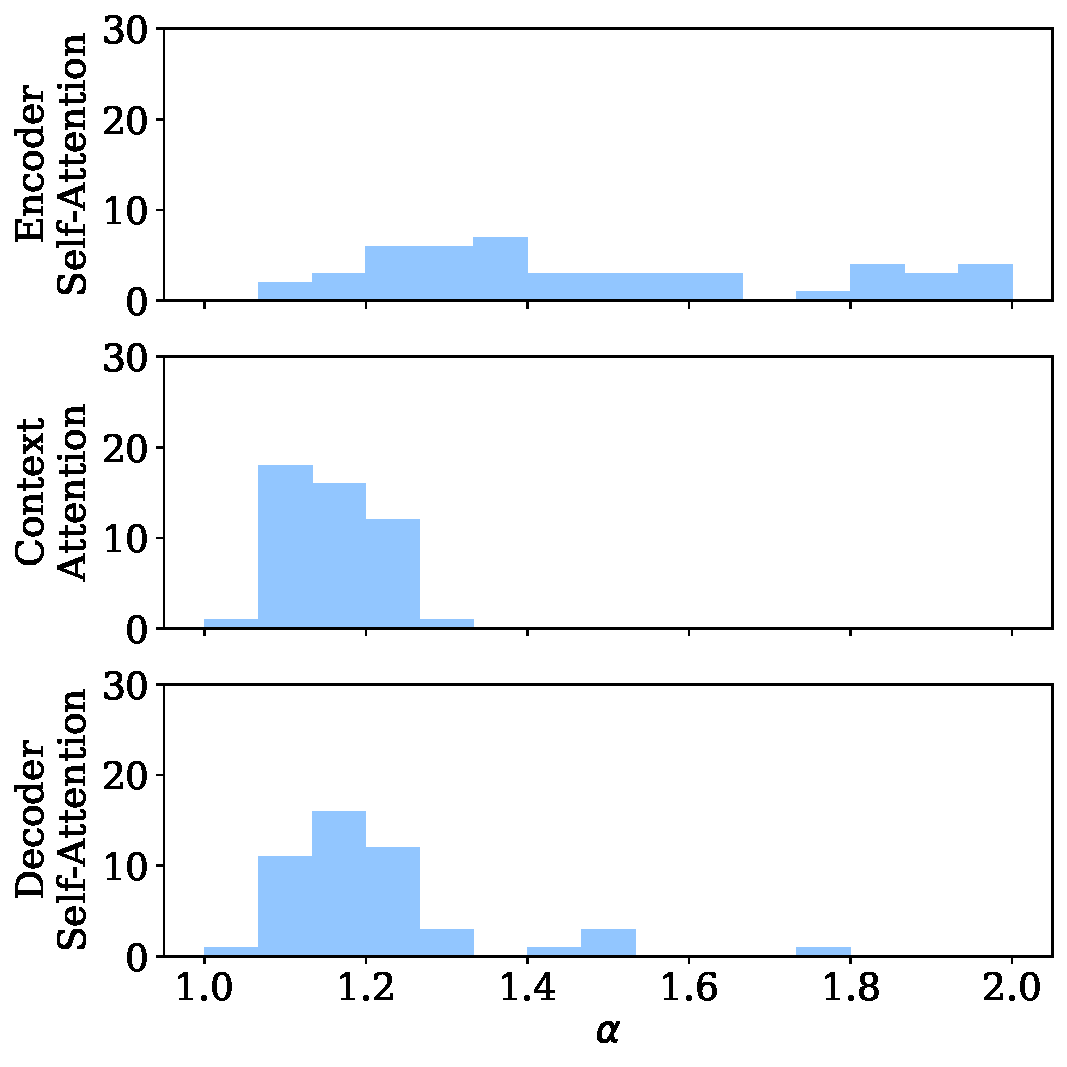
\includegraphics[width=\linewidth]{Figures/hist_alphas_ro.pdf}
        \caption{%
            \label{fig:hist_alphas_ro}%
            WMT 2016 \langp{ro}{en}.}
    \end{subfigure}
    \begin{subfigure}[b]{.49\linewidth}
        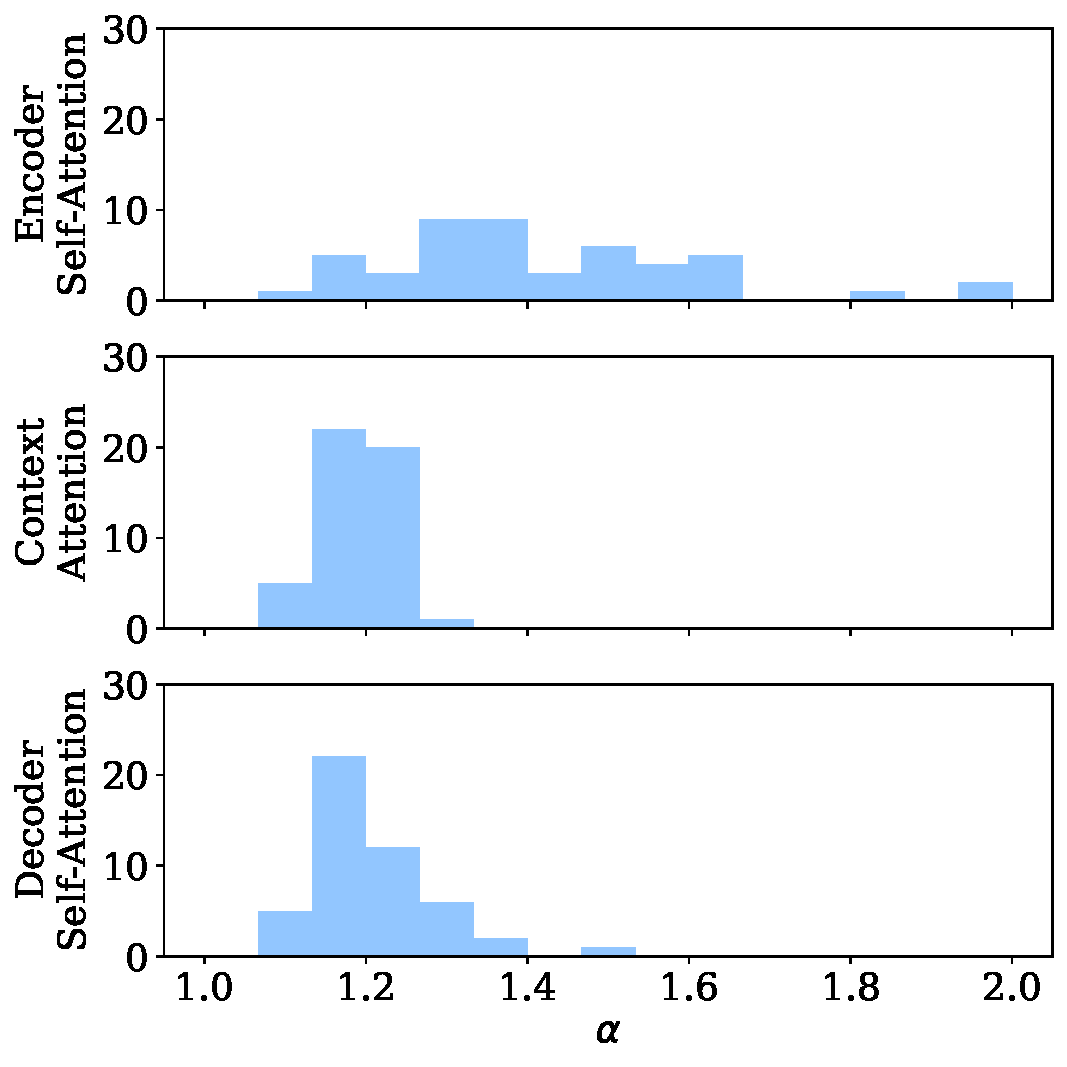
\includegraphics[width=\linewidth]{Figures/hist_alphas_ja.pdf}
        \caption{%
            \label{fig:hist_alphas_ja}%
            KFTT \langp{ja}{en}.}
    \end{subfigure}

    \begin{subfigure}[b]{.49\linewidth}
        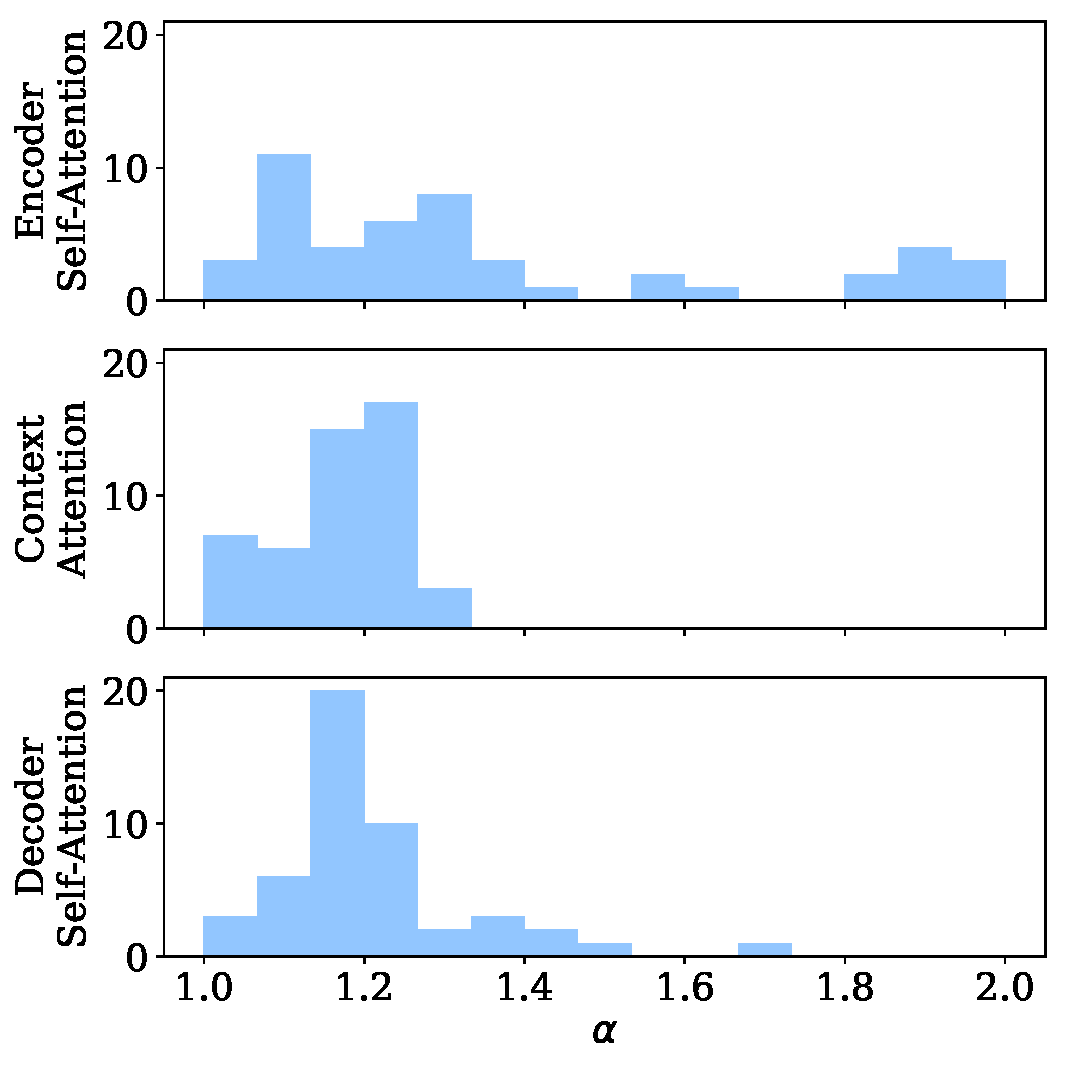
\includegraphics[width=\linewidth]{Figures/hist_alphas.pdf}
        \caption{%
            \label{fig:hist_alphas_en}%
            WMT 2014 \langp{en}{de}.}
    \end{subfigure}
    \begin{subfigure}[b]{.49\linewidth}
        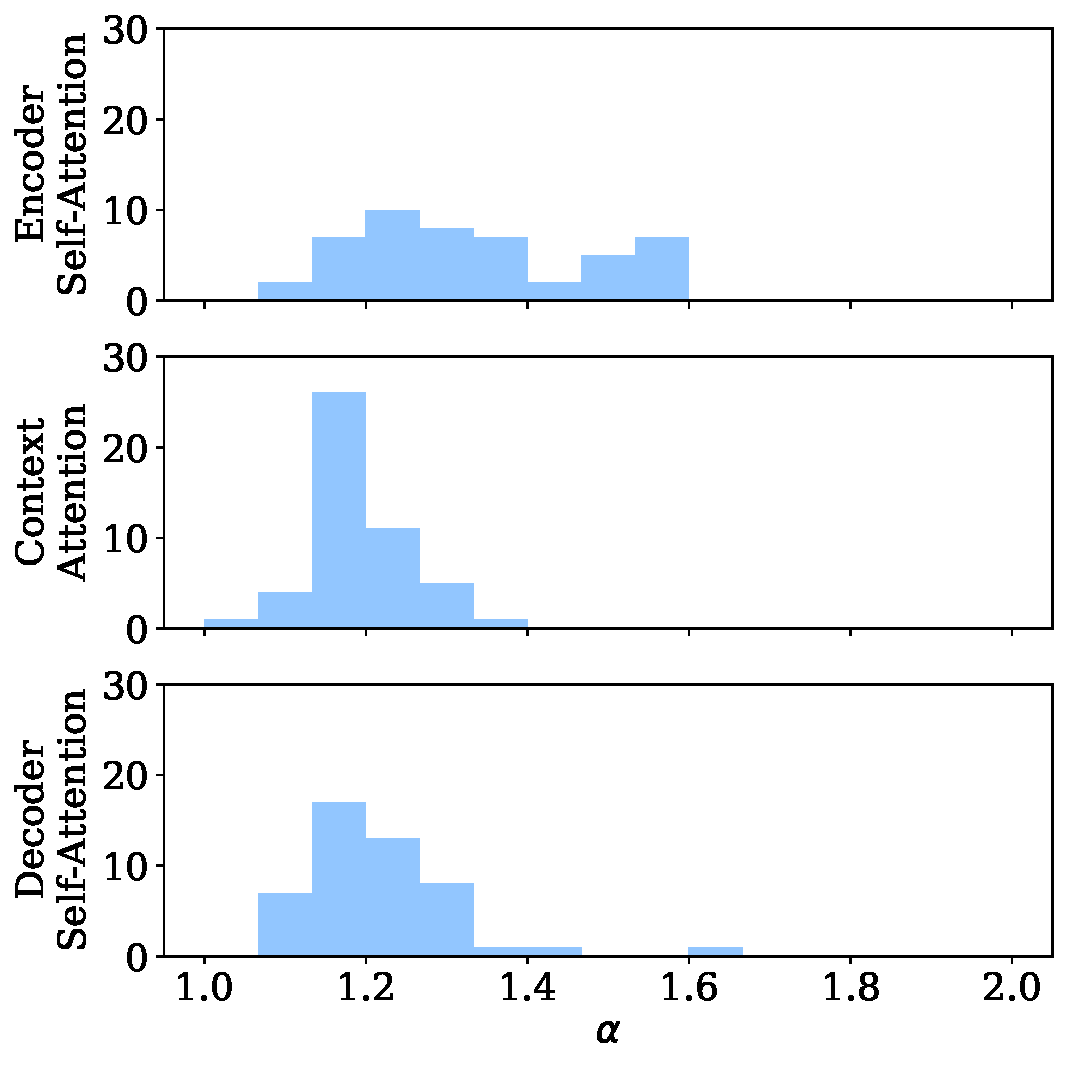
\includegraphics[width=\linewidth]{Figures/hist_alphas_de.pdf}
        \caption{%
            \label{fig:hist_alphas_de}%
            IWSLT 2017 \langp{de}{en}.}
    \end{subfigure}
    \caption{
        Distribution of learned $\alpha$ values per attention block.
        While the encoder self-attention has a bimodal distribution
        of values of $\alpha$,
        the decoder self-attention and context attention have a single mode.}
    \label{fig:hist_alphas}
\end{figure}

\begin{figure}[!htbp]
    \centering
    \begin{subfigure}[b]{.48\linewidth}
        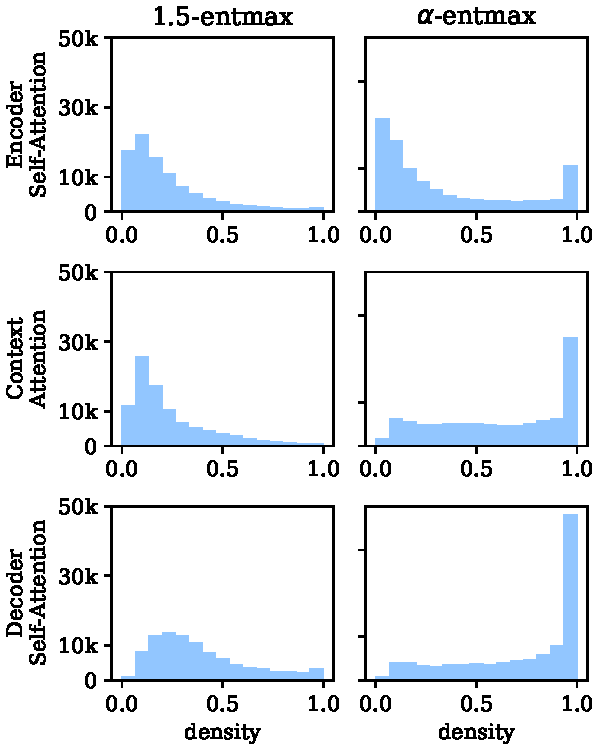
\includegraphics[width=\linewidth]{Figures/hist_densities_ro.pdf}
        \caption{%
            \label{fig:hist_densities_ro}%
            WMT 2016 \langp{ro}{en}.}
    \end{subfigure}
    \begin{subfigure}[b]{.48\linewidth}
        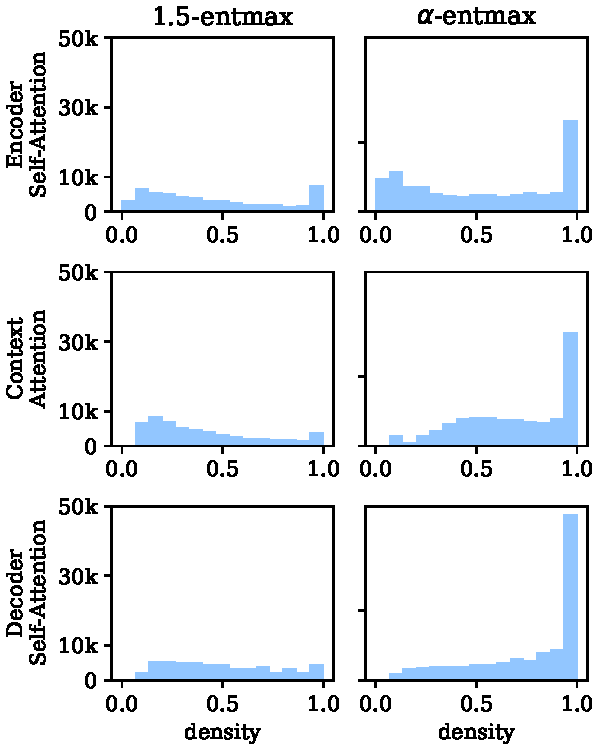
\includegraphics[width=\linewidth]{Figures/hist_densities_ja.pdf}
        \caption{%
            \label{fig:hist_densities_ja}%
            KFTT \langp{ja}{en}.}
    \end{subfigure}

    \begin{subfigure}[b]{.48\linewidth}
        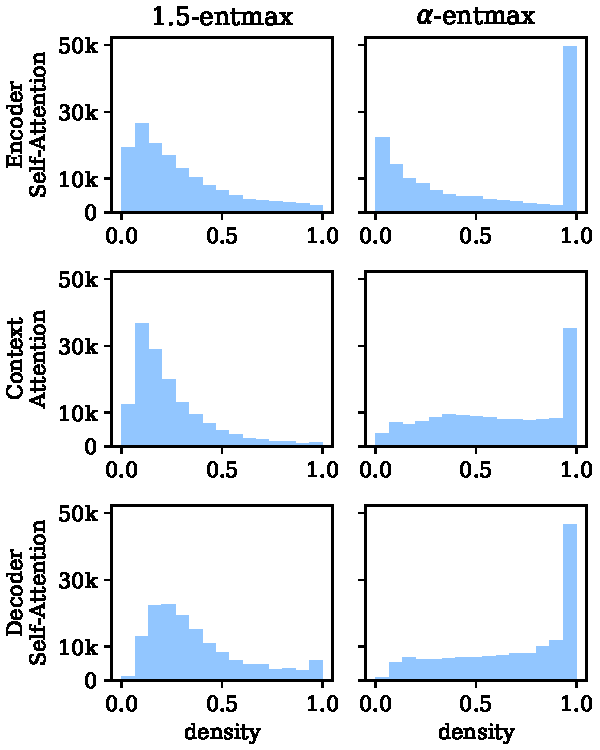
\includegraphics[width=\linewidth]{Figures/hist_densities.pdf}
        \caption{%
            \label{fig:hist_densities_en}%
            WMT 2014 \langp{en}{de}.}
    \end{subfigure}
    \begin{subfigure}[b]{.48\linewidth}
        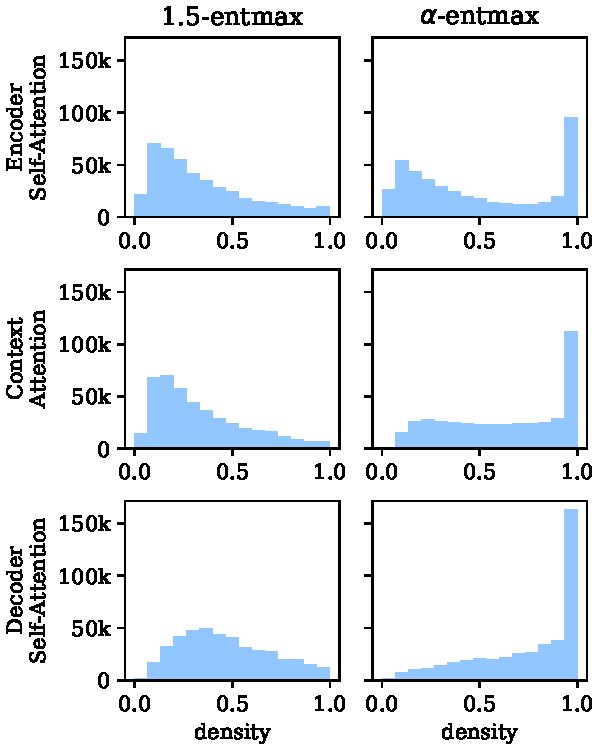
\includegraphics[width=\linewidth]{Figures/hist_densities_de.pdf}
        \caption{%
            \label{fig:hist_densities_de}%
            IWSLT 2017 \langp{de}{en}.}
    \end{subfigure}
    \caption{%
        \label{fig:hist_densities}
        Distribution of attention densities (average number of tokens
        receiving non-zero attention weight) for all attention heads and all
        validation sentences.
        When compared to 1.5-\entmaxtext{}, $\alpha$-\entmaxtext{}
        distributes the sparsity in a more uniform manner, with a clear mode
        at fully dense attentions, corresponding to the heads with low
        $\alpha$. In the softmax case, this distribution would lead to a
        single bar with density 1.}
\end{figure}

\paragraph*{Attention weight density when translating.}
For any $\alpha>1$, it would still be possible for the weight
matrices in \eqnref{eq:head} to learn re-scalings so as to make
attention sparser or denser. To visualize the impact of adaptive
$\alpha$ values, we compare the empirical attention weight density
(the average number of tokens receiving non-zero attention) within
each module, against sparse transformers with fixed $\alpha=1.5$.

\begin{sloppypar}
    \figref{fig:hist_densities} shows that, with fixed $\alpha=1.5$, heads
    tend to be sparse and similarly-distributed in all three attention
    modules. With learned $\alpha$, there are two notable changes: (i) a
    prominent mode corresponding to fully dense probabilities, showing
    that our models learn to combine sparse and dense attention, and (ii)
    a distinction between the encoder self-attention -- whose background
    distribution tends toward extreme sparsity -- and the other two
    modules, who exhibit more uniform background distributions. This
    suggests that perhaps entirely sparse transformers are suboptimal.
\end{sloppypar}

The fact that the decoder seems to prefer denser attention
distributions might be attributed to it being auto-regressive, only
having access to past tokens and not the full sentence. We speculate
that it might lose too much information if it assigned weights of
zero to too many tokens in the self-attention, since there are fewer
tokens to attend to in the first place.

Teasing this down into separate layers,
\figref{fig:head_density_per_layer} shows the average (sorted) density of
each head for each layer. We observe that $\alpha$-\entmaxtext{} is
able to learn different sparsity patterns at each layer, leading to
more variance in individual head behavior, to clearly-identified
dense and sparse heads, and overall to different tendencies compared
to the fixed case of $\alpha=1.5$.

\begin{figure}[!htbp]
    \centering
    \begin{subfigure}[b]{.49\linewidth}
        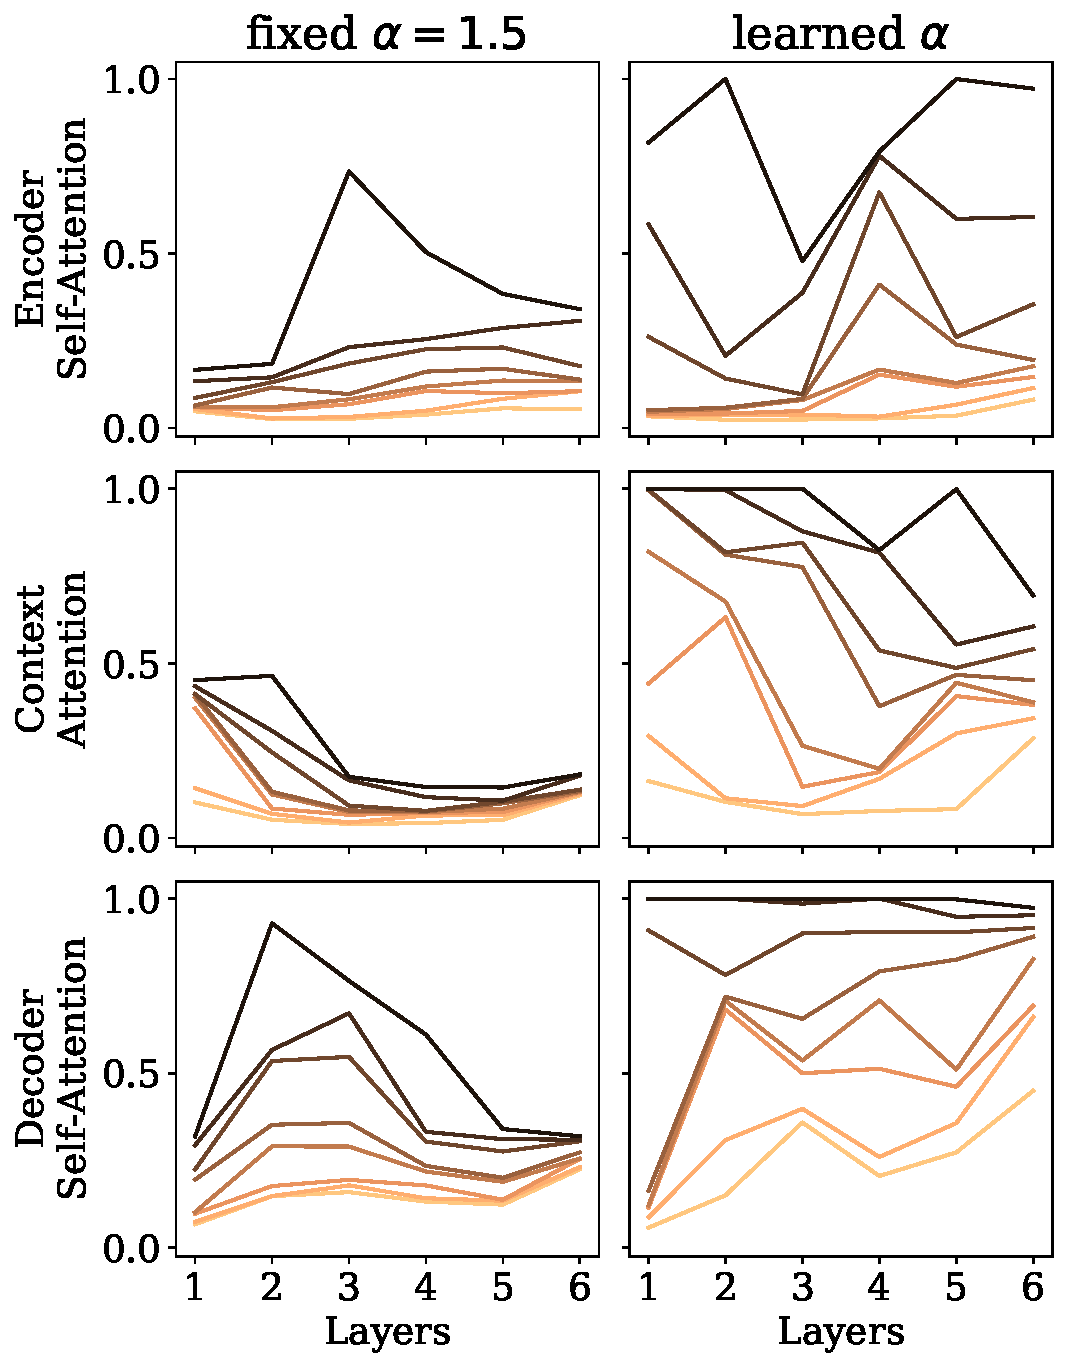
\includegraphics[width=\linewidth]{Figures/head_density_per_layer_ro.pdf}
        \caption{%
            \label{fig:head_density_per_layer_ro}%
            WMT 2016 \langp{ro}{en}.}
    \end{subfigure}
    \begin{subfigure}[b]{.49\linewidth}
        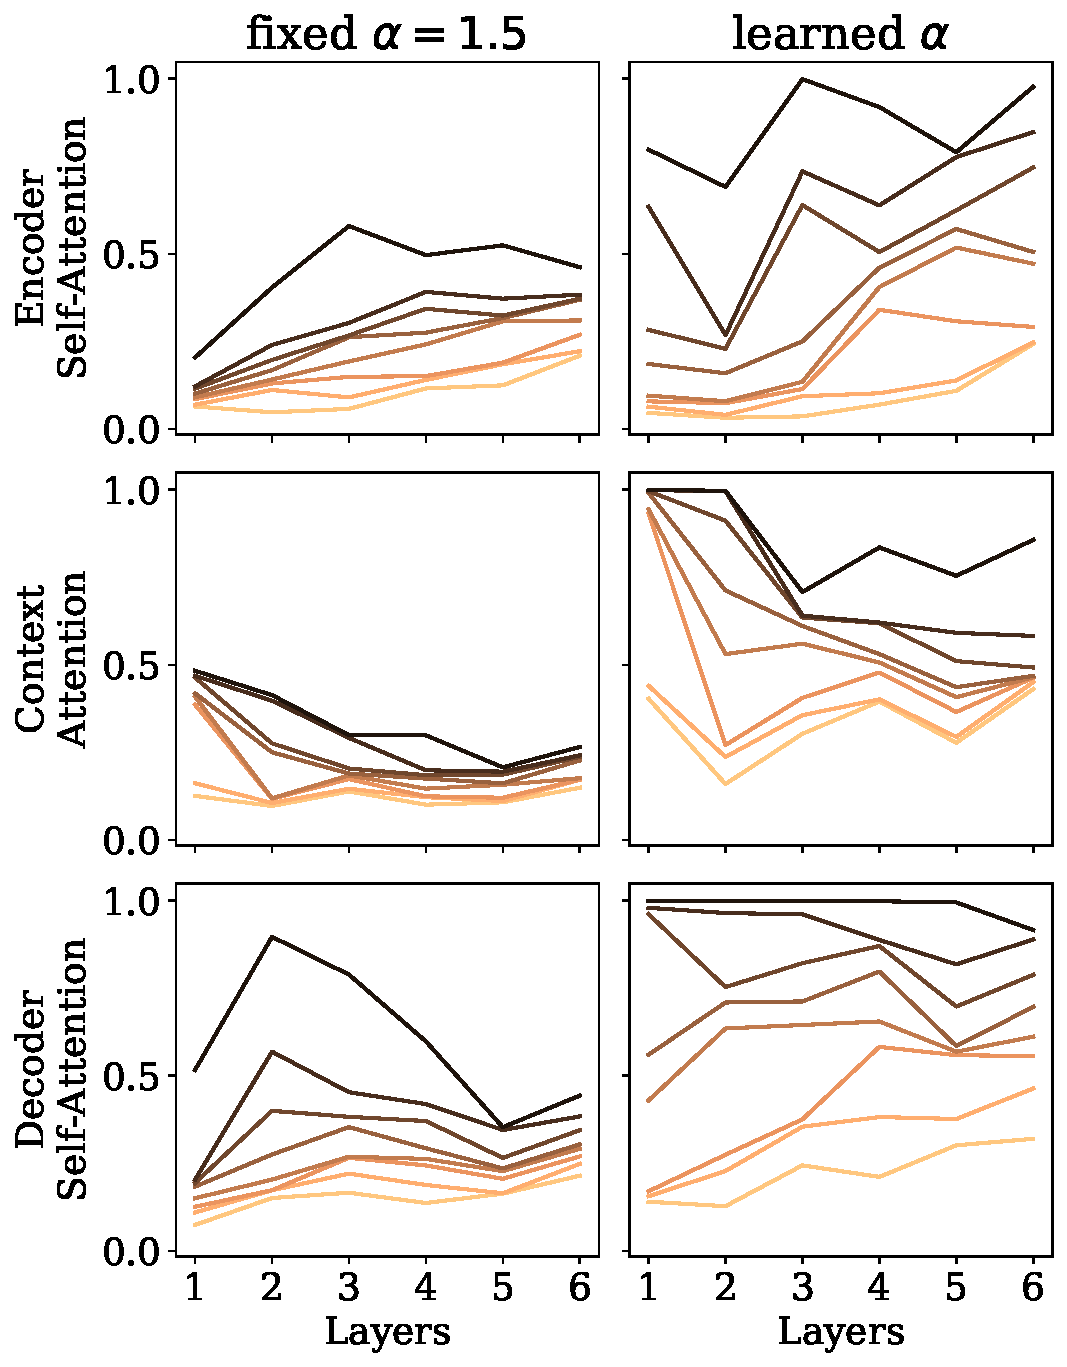
\includegraphics[width=\linewidth]{Figures/head_density_per_layer_ja.pdf}
        \caption{%
            \label{fig:head_density_per_layer_ja}%
            KFTT \langp{ja}{en}.}
    \end{subfigure}

    \begin{subfigure}[b]{.49\linewidth}
        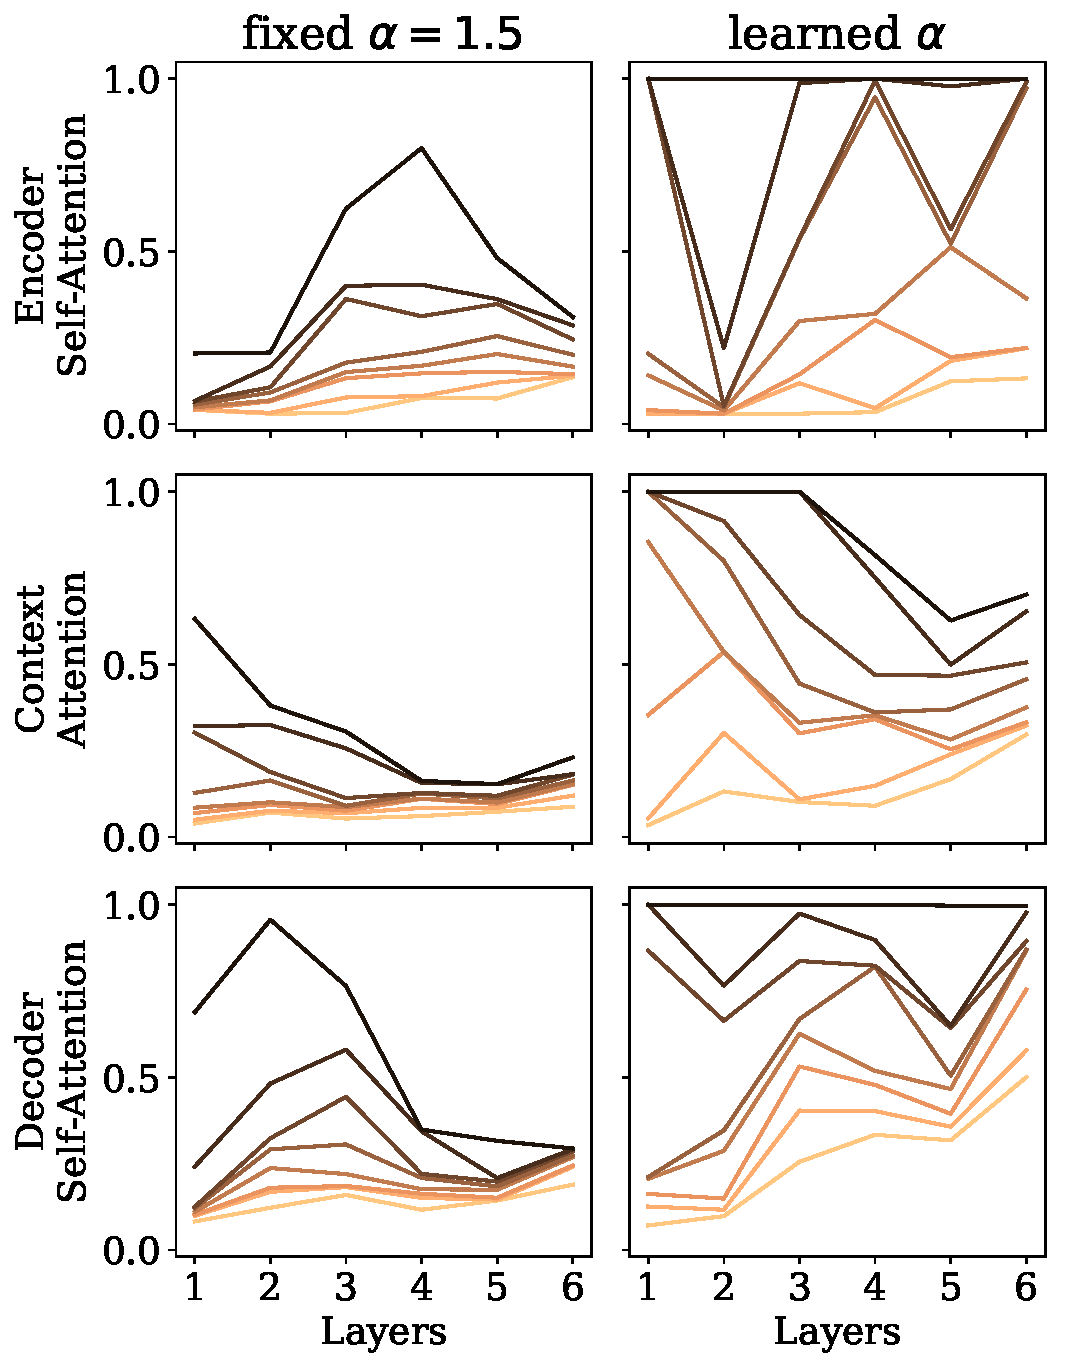
\includegraphics[width=\linewidth]{Figures/head_density_per_layer.pdf}
        \caption{%
            \label{fig:head_density_per_layer_en}%
            WMT 2014 \langp{en}{de}.}
    \end{subfigure}
    \begin{subfigure}[b]{.49\linewidth}
        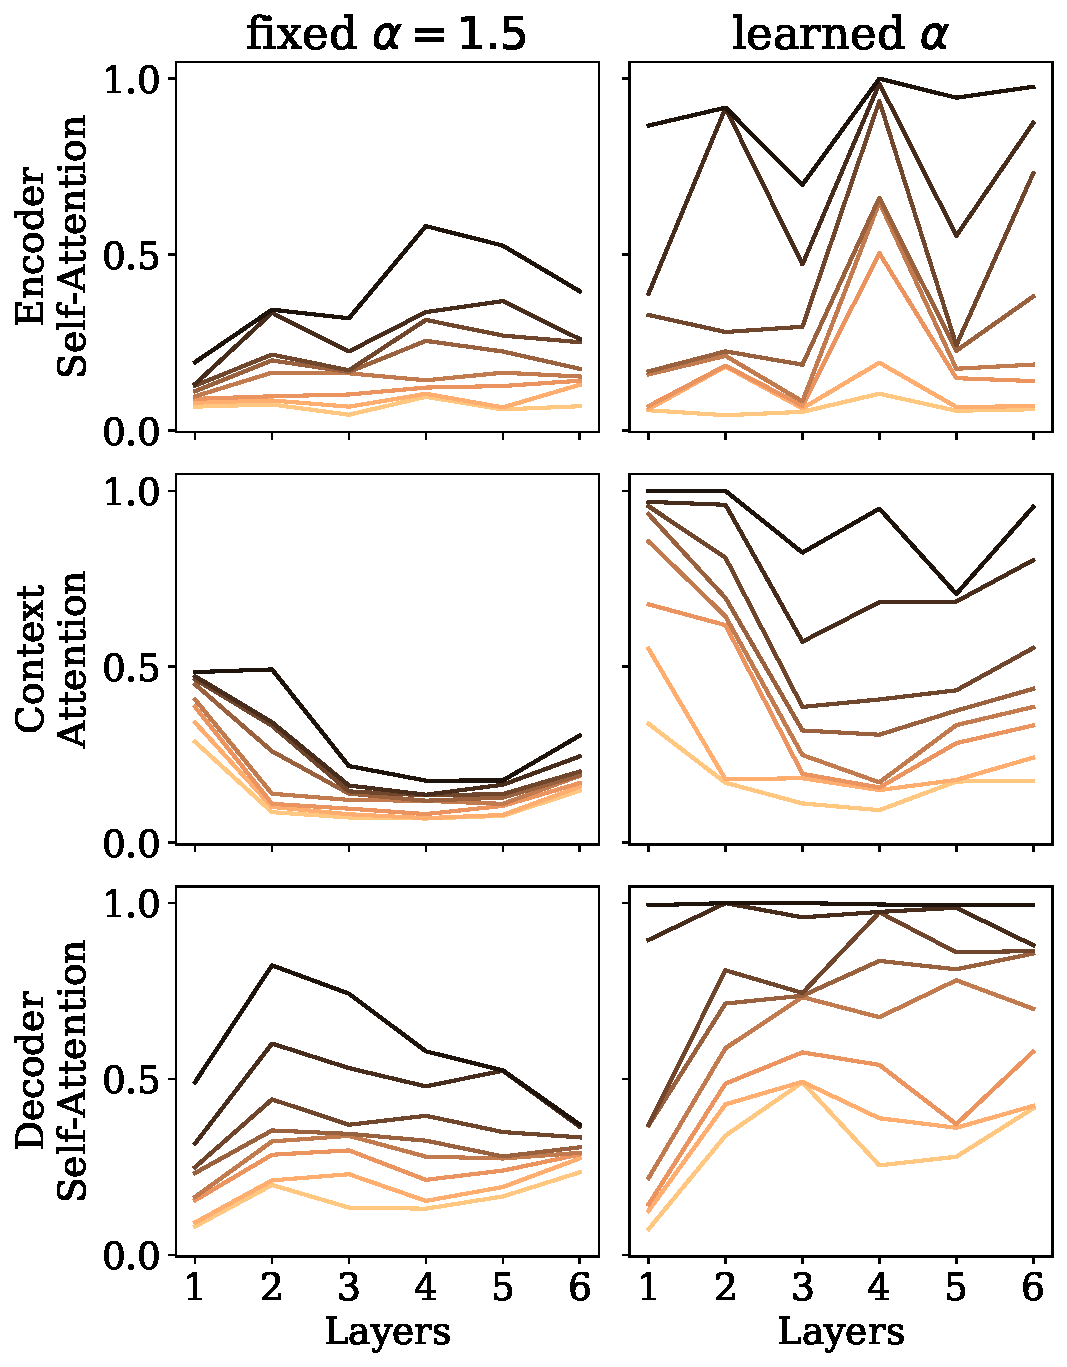
\includegraphics[width=\linewidth]{Figures/head_density_per_layer_de.pdf}
        \caption{%
            \label{fig:head_density_per_layer_de}%
            IWSLT 2017 \langp{de}{en}.}
    \end{subfigure}
    \caption{%
        \label{fig:head_density_per_layer}
        Head density per layer for fixed and learned $\alpha$. Each line
        corresponds to an attention head; lower values mean that that
        attention head is sparser. Learned $\alpha$ has higher variance.
    }
\end{figure}

\begin{figure}[!htbp]
    \centering
    \begin{subfigure}[b]{.49\linewidth}
        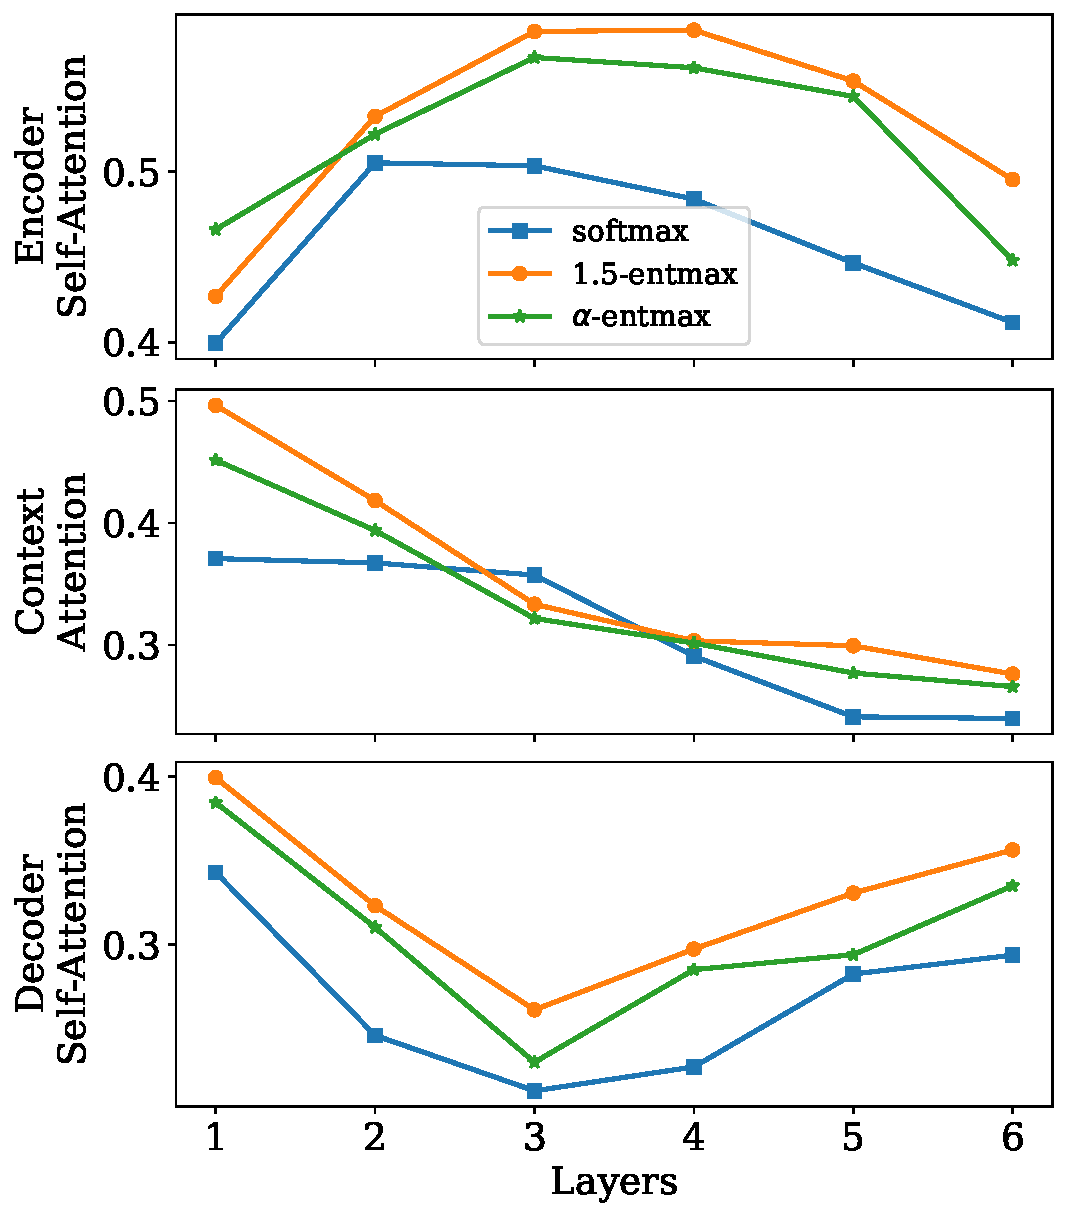
\includegraphics[width=\linewidth]{Figures/js_divs_ro.pdf}
        \caption{%
            \label{fig:js_divs_ro}%
            WMT 2016 \langp{ro}{en}.}
    \end{subfigure}
    \begin{subfigure}[b]{.49\linewidth}
        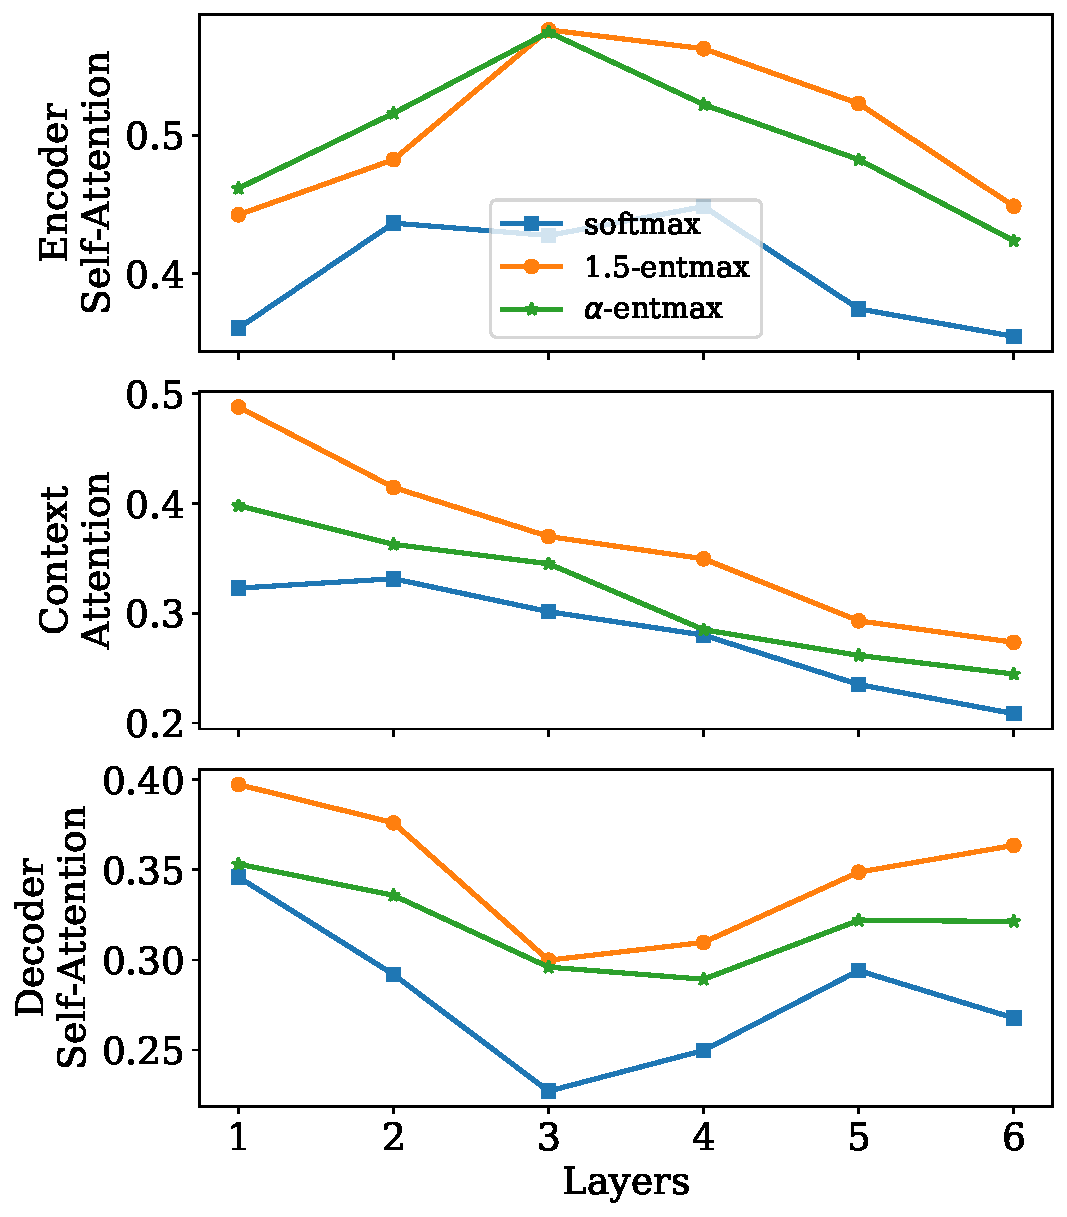
\includegraphics[width=\linewidth]{Figures/js_divs_ja.pdf}
        \caption{%
            \label{fig:js_divs_ja}%
            KFTT \langp{ja}{en}.}
    \end{subfigure}

    \begin{subfigure}[b]{.49\linewidth}
        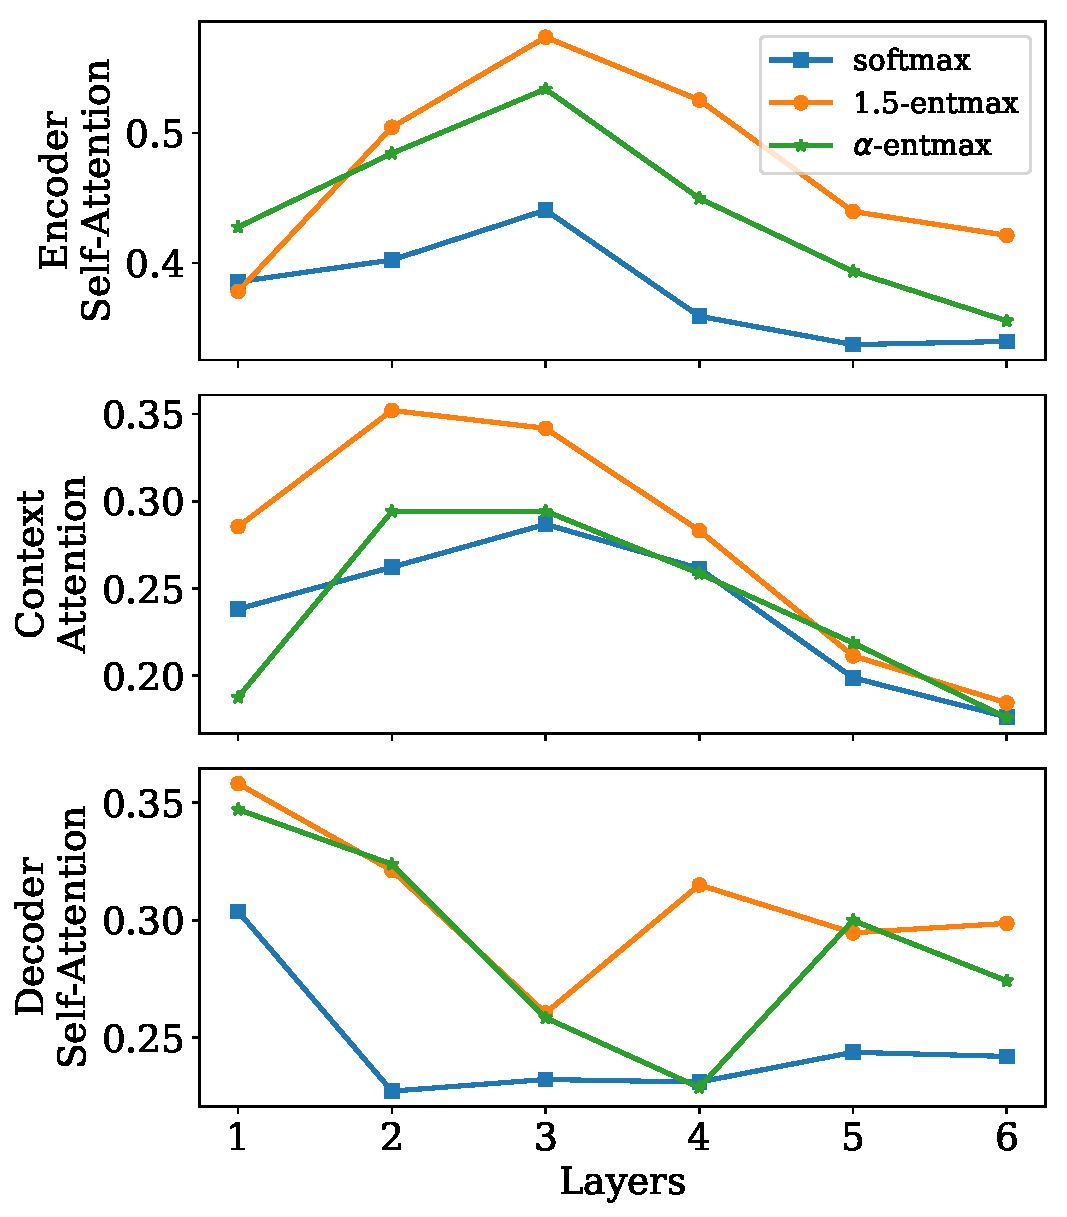
\includegraphics[width=\linewidth]{Figures/js_divs.pdf}
        \caption{%
            \label{fig:js_divs_en}%
            WMT 2014 \langp{en}{de}.}
    \end{subfigure}
    \begin{subfigure}[b]{.49\linewidth}
        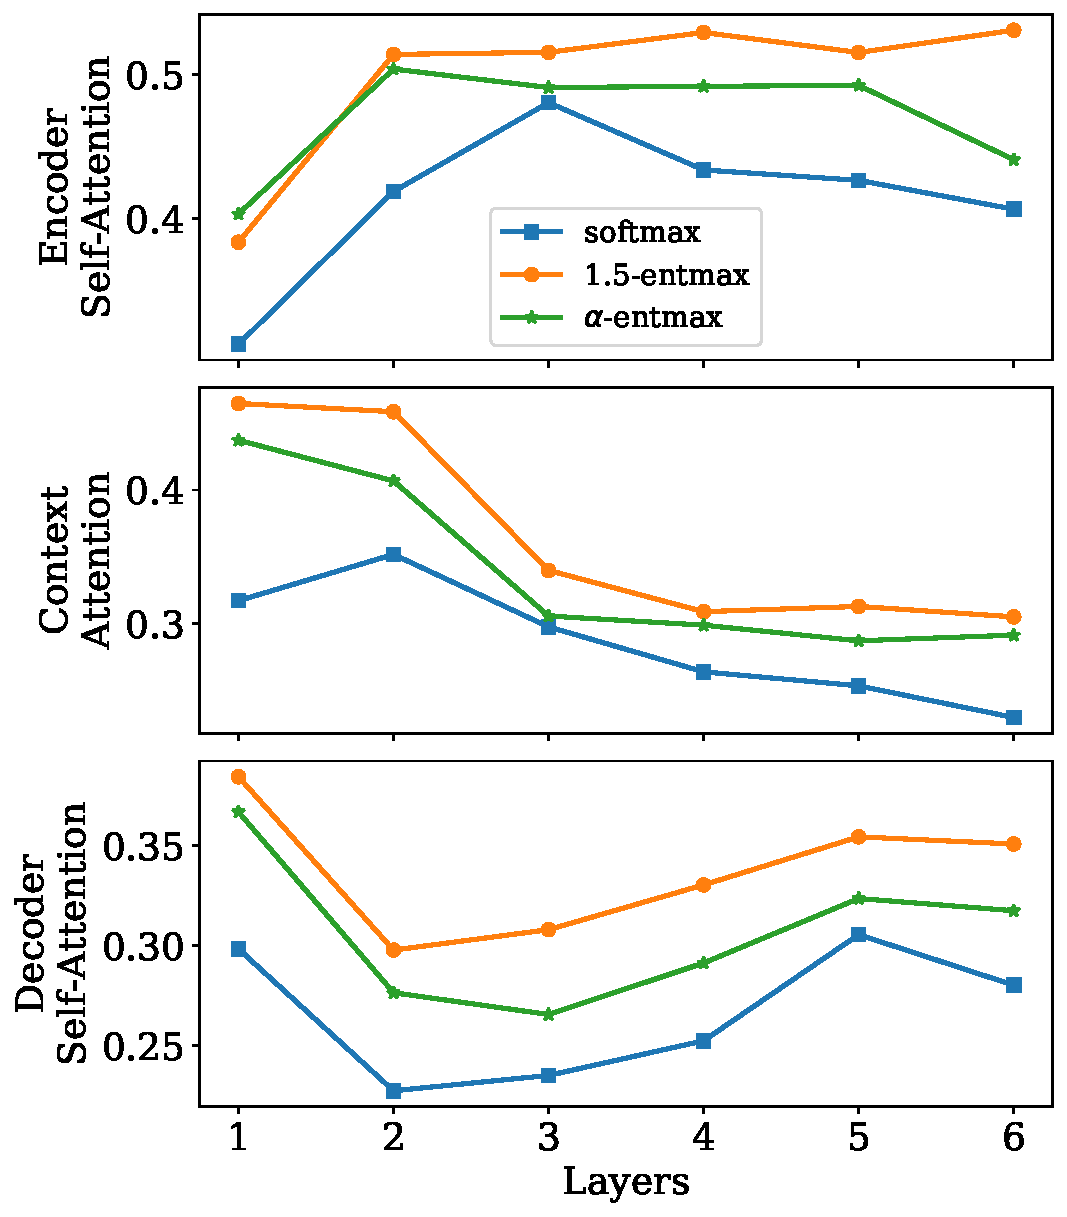
\includegraphics[width=\linewidth]{Figures/js_divs_de.pdf}
        \caption{%
            \label{fig:js_divs_de}%
            IWSLT 2017 \langp{de}{en}.}
    \end{subfigure}
    \caption{%
        \label{fig:js_divs}
        Jensen-Shannon Divergence between heads at each layer. Measures the
        disagreement between heads: the higher the value, the more the heads
        are disagreeing with each other in terms of where to attend. Models
        using sparse \entmaxtext have more diverse attention than the softmax
        baseline.
    }
\end{figure}

\paragraph*{Head diversity.} To measure the overall disagreement
between heads, as a measure of head diversity, we use the
following generalization of the Jensen-Shannon divergence:
%
\begin{equation}
    JS = \HHs\left(\frac{1}{H}\sum_{j=1}^H \bm{p}_{j}\right) -
    \frac{1}{H}\sum_{j=1}^{H}
    \HHs(\bm{p}_j)
\end{equation}
%
where $\bm{p}_j$ is the vector of attention weights assigned by head
$j$ to each word in the sequence, and $\HHs$ is the Shannon entropy,
base-adjusted based on the dimension of $\bm{p}$ such that $JS \leq
    1$. We average this measure over the entire validation set. The
higher this metric is, the more the heads are taking different roles
in the model.

\figref{fig:js_divs} shows that both sparse transformer variants show
more diversity than the traditional softmax one. Interestingly,
diversity seems to often peak in the middle layers of the encoder
self-attention and context attention, while this is not the case for
the decoder self-attention.

\begin{figure}[htbp]
    \centering
    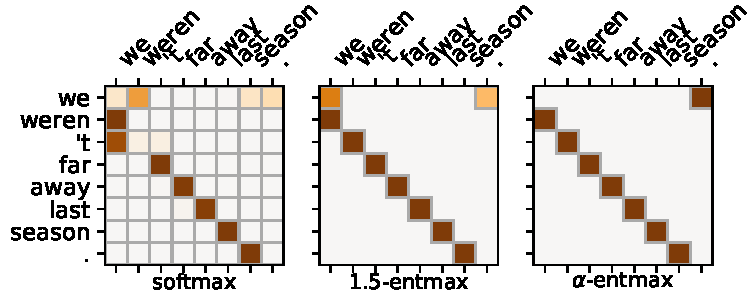
\includegraphics[width=0.95\columnwidth]{Figures/head_prev.pdf}
    \caption{
        Self-attention from the most confidently previous-position head in
        each model. The learned parameter in the $\alpha$-\entmaxtext model
        is $\alpha=1.91$. Quantitatively more confident, visual inspection
        confirms that the adaptive head behaves more consistently.}
    \label{fig:head_prev}
\end{figure}

\begin{figure}[htbp]
    \centering
    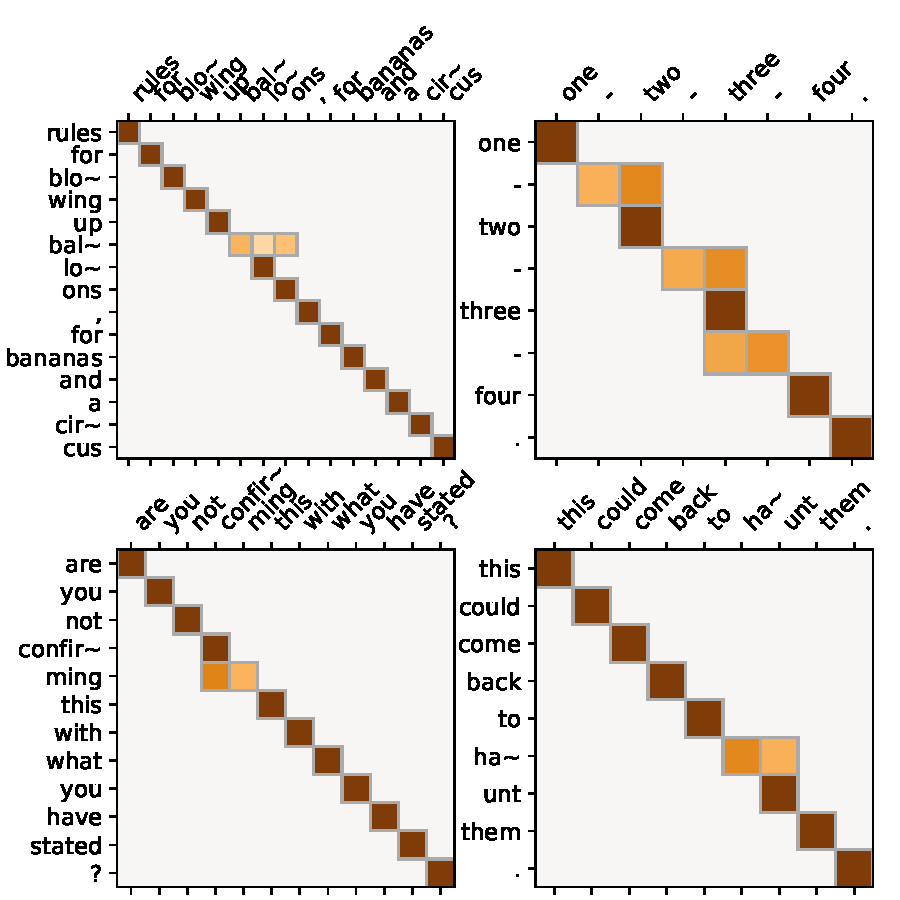
\includegraphics[width=0.95\columnwidth]{Figures/head_bpe}
    \caption{%layer 5+1 / head 6+1, alpha=1.33.
        BPE-merging head $(\alpha=1.91)$ discovered in the
        $\alpha$-\entmaxtext model. Found in the first encoder layer,
        this head learns to discover some subword units and combine their
        information, leaving most words intact. It places $99.09\%$ of
        its probability mass within the same BPE cluster as the current
        token: more than any head in any other model.}
    \label{fig:head_bpe}
\end{figure}

\begin{figure}[htbp]
    \centering
    \begin{subfigure}[b]{0.95\columnwidth}
        \centering
        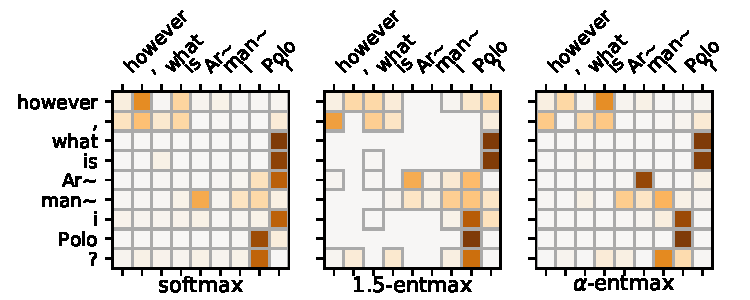
\includegraphics[width=\columnwidth]{Figures/head_interro.pdf}
    \end{subfigure}
    \begin{subfigure}[b]{0.95\columnwidth}
        \centering
        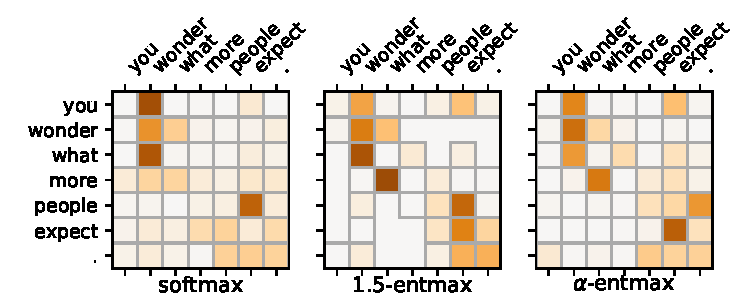
\includegraphics[width=\columnwidth]{Figures/head_interro_not.pdf}
    \end{subfigure}
    \caption{%layer 0+1 head 2+1 alpha=1.05
        Interrogation-detecting heads in the three models. The top sentence
        is interrogative while the bottom one is declarative but includes the
        interrogative word ``what''. In the top example, these {\it
                interrogation heads} assign a high probability to the question mark
        in the time step of the interrogative word (with $\geq 97.0\%$
        probability), while in the bottom example since there is no question
        mark, the same head does not assign a high probability to the last
        token in the sentence during the interrogative word time step.
        Surprisingly, this head prefers a low $\alpha=1.05$, as can be seen
        from the dense weights. This allows the head to identify the noun
        phrase ``Armani Polo" better.}
    \label{fig:head_interro}
\end{figure}

\begin{figure}[htbp]
    \centering
    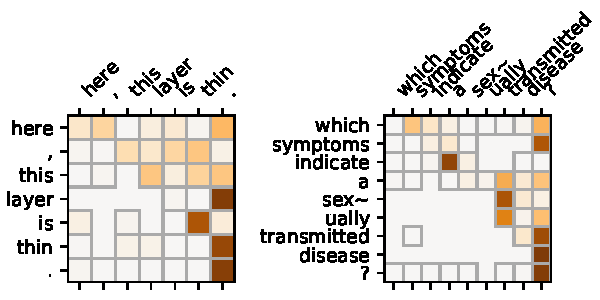
\includegraphics[
        width=0.95\columnwidth]{Figures/sparsity_difference.pdf}
    \caption{%layer 5+1 / head 6+1, alpha=1.33.
        Example of two sentences of similar length where the same head
        ($\alpha=1.33$) exhibits different sparsity. The longer phrase in the
        example on the right ``a sexually transmitted disease'' is handled
        with higher confidence, leading to more sparsity.
    }
    \label{fig:sparsity_difference}
\end{figure}

\subsection{Identifying Head Specializations}\label{sec:spec}

\noindent Previous work pointed out some specific roles played by
different heads in the softmax transformer
model~\citep{voita2018context,tang2018why,specialized}. Identifying
the specialization of a head can be done by observing the
type of tokens or sequences that the head often assigns most
of its attention weight; this is facilitated by sparsity.

\paragraph*{Positional heads.}
One particular type of head, as noted by \citet{specialized}, is the
positional head. These heads tend to focus their attention on either
the previous or next token in the sequence, thus obtaining
representations of the neighborhood of the current time step. In
\figref{fig:head_prev}, we show attention plots for such heads, found for
each of the studied models. The sparsity of our models allows these
heads to be more confident in their representations, by assigning the
whole probability distribution to a single token in the sequence.
Concretely, we may measure a positional head's \textbf{confidence} as
the average attention weight assigned to the previous token. The
softmax model has three heads for position $-1$, with median
confidence $93.5\%$. The $1.5$-\entmaxtext model also has three heads
for this position, with median confidence $94.4\%$. The adaptive
model has four heads, with median confidences $95.9\%$, the
lowest-confidence head being dense with $\alpha=1.18$, while the
highest-confidence head being sparse ($\alpha=1.91$).

For position $+1$, the models each dedicate one head, with confidence
around $95\%$, slightly higher for \entmaxtext. The adaptive model
sets $\alpha=1.96$ for this head.

\paragraph*{BPE-merging head.}
Due to the sparsity of our models, we are able to identify other head
specializations, easily identifying which heads should be further analyzed.
In \figref{fig:head_bpe} we show one such head where the $\alpha$ value
is particularly high (in the encoder, layer 1, head 4 depicted in
\figref{fig:learning_alpha}). We found that this head most often looks at
the current time step with high confidence, making it a positional head
with offset $0$. However, this head often spreads weight sparsely
over 2-3 neighboring tokens, when the tokens are part of the same BPE
cluster\footnote{BPE-segmented words are denoted by $\sim$ in the
    Figures.} or hyphenated words. As this head is in the first layer, it
provides a useful service to the higher layers by combining
information evenly within some BPE clusters.

For each BPE cluster or cluster of hyphenated words,
we computed a score between 0 and 1 that corresponds to the
maximum attention mass assigned by any token to the rest of the
tokens inside the cluster in order to quantify the BPE-merging
capabilities of these heads.\footnote{If the
    cluster has size 1, the score is the weight the token assigns to
    itself.} There are not any attention heads in
the softmax model that are able to obtain a score over $80\%$, while
for $1.5$-\entmaxtext and $\alpha$-\entmaxtext there are two heads
in each ($83.3\%$ and $85.6\%$ for $1.5$-\entmaxtext and $88.5\%$ and
$89.8\%$ for $\alpha$-\entmaxtext).

\paragraph*{Interrogation head.}
On the other hand, in \figref{fig:head_interro} we show a head for which our
adaptively sparse model chose an $\alpha$ close to 1, making it
closer to softmax (also shown in {\it encoder, layer 1, head 3}
depicted in \figref{fig:learning_alpha}). We observe that this head
assigns a high probability to question marks at the end of the
sentence in time steps where the current token is interrogative, thus
making it an interrogation-detecting head. We also observe this type
of heads in the other models, which we also depict in
\figref{fig:head_interro}. The average attention weight placed on the
question mark when the current token is an interrogative word is
$98.5\%$ for softmax, $97.0\%$ for $1.5$-\entmaxtext, and $99.5\%$
for $\alpha$-\entmaxtext.

Furthermore, we can examine sentences where some tendentially sparse
heads become less so, thus identifying sources of ambiguity where the
head is less confident in its prediction. An example is shown in
\figref{fig:sparsity_difference} where sparsity in the same head differs
for sentences of similar length.

\section{Subsequent Work}\label{sec:subsequent_work_adapt}

\noindent \citet{correia2019adaptively} is part of an early line of work
on transformers that sparked interest in making this model more
efficient~\citep[\textit{inter
        alia}]{daras2020SMYRFEfficientAttention,
    li2020SACAcceleratingStructuring, merrill2021EffectsParameterNorm,
    roy2021EfficientContentBasedSparse}, using sparsity to allow for
transformers to use longer contexts more
effectively~\citep[\textit{inter alia}]{jiang2020LongDocumentRanking,
    qiu2020BlockwiseSelfAttentionLong, sukhbaatar2021NotAllMemories}, and
being able to understand transformers better~\citep[\textit{inter
        alia}]{you2020HardCodedGaussianAttention,
    rogers2020PrimerBERTologyWhat, pande2021headshypothesisunifying}.
This transformer variant and $\alpha$-\entmaxtext have also proved
useful in medical applications~\citep{guo2020LearningLatentForests,
    yun2021SpecTrSpectralTransformer}.

Particularly connected to the present work,
\citet{treviso2021PredictingAttentionSparsity} tackles the quadratic
complexity that remains in our approach, as we had focused more on
the interpretability benefits of sparsity and not on its potential
computational benefits.
\citet{treviso2021PredictingAttentionSparsity} propose
\emph{Sparsefinder}, a method that predicts in advance the sparsity
pattern of $\alpha$-\entmaxtext, by projecting queries and keys into
a lower dimensional space, turning our approach into a
computationally efficient alternative to the original transformer.

Still on the topic of computational efficiency,
\citet{ji2021DistributionSparsityInferencetime} focuses on inducing
sparsity on the attention heads only at inference time to avoid
unecessary training of new models and wasting of computational
resources. In order to achieve this, they propose a pruning and
quantization technique that does not lead to decreased performance.
To push the sparsity to the limit,
\citet{xu2021LearningHardRetrieval} propose a hard retrieval approach
that is able to make each attention mechanism attend to only a single
token. This approach also leads to similar performance to the
original transformer but ends up having a 1.43 times faster decoding
performance in translation tasks.

Regarding the concept of Sparse transformers,
\citet{yun2020ConnectionsareExpressive} unify several works that
sparsify transformers in a single framework.
This unified framework is constructed through conditions based on the
sparsity pattern and the probability map. Once such conditions are
satisfied, the authors prove that some sparse transformers (of which
our approach is included) are universal approximators of any
continuous sequence-to-sequence function. Furthermore, they show that
when these sparse transformers have only $\mathcal{O}(n)$ connections (which is
in contrast to the constant $\mathcal{O}(n^2)$ connections of dense
transformers), they still hold the same universal approximation
properties.

\citet{zhang2021SparseAttentionLinear} proposed another approach to
induce sparsity in each attention head of the transformer. In this
work, instead of replacing the softmax with entmax, the authors
replace it with the ReLU activation. When compared to our approach,
Rectified Linear Attention (ReLA) obtains faster training and
decoding time, while achieving close performance in translation
tasks. In their analysis, they followed our methodology and found
that their method had higher JS Divergence than our own, suggesting
that attention heads using ReLA tend to be more diverse in where they
attend at each layer. Furthermore, ReLA is also able to assign null
attention for some queries, that is, to effectively deactivate an
attention head for a specific query, as it is able to assign zero
values to all tokens. Their analysis shows that the rate at which
null attention happens increases in deeper layers, which correlates
with our own analysis that deeper layers contain less information.
Moreover, \citet{zhang2021SparsifyingEncoderOutputs} achieves
sparsity by pruning entire sections of the encoder outputs in the
cross-attention of the decoder. This leads to a significant speed-up
during decoding. It drops whole sections from the source encodings to
speed up decoding, and the authors find that the tokens that end up
being dropped are often uninformative tokens, while the retained ones
are relatively rare.

On the topic of interpretability and understanding the inner workings
of transformers, inspired by our analysis along with other
works~\citep{specialized} that find that
encoder self-attention heads learn fixed patterns
(\secref{sec:spec}), \citet{raganato2020FixedEncoderSelfAttention}
fixes the attention pattern of all but one head in each layer,
letting only a single head in each layer learn its attention. Those
fixed patterns include the positional heads that focus on the
current, previous, and next token and the BPE-merging head that we
found. The parameter footprint of the model drastically decreases
thanks to these simplifications, and the authors show empirically
that translation quality does not drop significantly and even that,
in low-resource scenarios, this approach improves translation
performance.

\section{Final Remarks and Chapter Summary}

In the present chapter, we contributed with a novel strategy for
\textbf{learnable sparse} attention, and, in particular, for adaptively
sparse transformers. We presented the first empirical analysis of
transformers with sparse attention mappings (\ie, \entmaxtext),
showing potential in both translation accuracy as well as in model
interpretability.

In particular, we analyzed how the attention heads in the adaptively
sparse transformer can specialize more and with higher confidence.
Our adaptivity strategy relies only on gradient-based optimization,
side-stepping costly per-head hyperparameter searches. Given the
impact of our work, we believe that similar approaches will continue
to increase in the future, and improving neural
models' efficiency and \textbf{transparency}.

\cleardoublepage

\singlespacing
\fancychapter[Efficient Marginalization of Discrete and Structured Latent Variables via Sparsity]{Efficient Marginalization of Discrete and Structured Latent Variables}
\label{chap:sparsemarg}

\cleardoublepage
\doublespacing

In this chapter, we focus on the objective of making neural models
more \textbf{compact}. We will propose a novel approach to train
discrete and structured latent variable models that achieves an exact
gradient unlike previous strategies in this field. Latent discrete
and structured variables are of particular interest for compactness
of neural models since they can constrain the model and provide
inductive bias. This family of latent variable models can also be easily
semi-supervised, which can further increase the inductive bias and
thus the compactness of the model.

The exactness of the gradient of our approach is achieved through
marginalization. As we shall see, it turns out to be efficient thanks
to parameterizing the distribution over categories or structures with
\textbf{sparsity}. Therefore, while in the previous chapter we have
used sparsity for increased transparency, we will now use sparsity
for increased efficiency. Albeit in a different way than in the
previous chapter, this sparsity will too be \textbf{learned} over
time, increasing as the training progresses due to the model being
more confident on latent variable assignments.

\textit{This chapter is based on \citet{correia2020procneurips}.}

\section{Motivation}
\label{sec:intro}

Training with discrete variables (\secref{sec:discrete_lvm_bg}) can
become challenging, due to the need to compute a gradient of a large
sum over all possible latent variable assignments, with each term
itself being potentially expensive. This challenge is typically
tackled by estimating the gradient with Monte Carlo
methods~\citep[MC;][]{mohamed2019monte}, which rely on sampling
estimates. The two most common strategies for MC gradient estimation
are the score function
estimator~\citep[SFE;][]{rubinstein1976monte,paisley2012variational},
which suffers from high variance, or surrogate methods that rely on
the continuous relaxations, like straight-through~\citep{STE} or
Gumbel-Softmax~\citep{Concrete,GumbelSoftmax}, which potentially
reduce variance but introduce bias and modeling assumptions.

In this work, we take a step back and ask: Can we avoid sampling
entirely, and instead deterministically evaluate the sum with less
computation? To answer affirmatively, we propose an alternative
method to train these models by parameterizing the discrete
distribution with {\bf sparse
        mappings}\,---\,sparsemax~\citep{martins2016softmax} and two
structured counterparts, \smap~\citep{niculae2018sparsemap} and a
novel mapping top-$k$ sparsemax. Sparsity implies that some
assignments of the latent variable are entirely ruled out. This leads
to the corresponding terms in the sum evaluating trivially to zero,
allowing us to disregard potentially expensive computations.

\paragraph*{Contributions.} We introduce a general strategy for
learning discrete latent variable models that hinges on
learning a sparse distribution over the possible assignments. In the
unstructured categorical case our strategy relies on the sparsemax
activation function, presented in~\secref{sec:categorical}, while in the
structured case we propose two strategies, \smap and top-$k$
sparsemax, presented in~\secref{sec:structured}. Unlike existing
approaches, our strategies involve neither MC estimation nor any
relaxation of the discrete latent variable to the continuous space.
We demonstrate our strategy on three different applications: a
semi-supervised generative model, an emergent communication game, and
a bit-vector variational autoencoder. We provide a thorough analysis
and comparison to MC methods, and\,---\,when feasible\,---\,to exact
marginalization. Our approach is consistently a top performer,
combining the accuracy and robustness of exact marginalization with
the efficiency of single-sample estimators.

\section{Previous Work}

\paragraph*{Differentiable sparse mappings.} There has been recent
interest in applying sparse mappings of discrete distributions in
deep discriminative models~\citep{martins2016softmax,
    niculae2018sparsemap, fusedmax, entmax, sparsemapcg}, attention
mechanisms~\citep{malaviya2018sparse, shao2019ssn,
    maruf2019selective, correia2019adaptively}, and in topic
models~\citep{caothesis}. Our work focuses on the parameterization of
distributions over latent variables with sparse mappings, on the
computational advantage to be gained by sparsity, and on the contrast
between our novel training method and common sampling-based methods.

\paragraph*{Reducing sampling noise.} The sampling procedure found in
SFE is a great source of variance in models that use it.
To reduce this variance, many works have proposed
baselines~\citep{Williams1992,MuProp,CV2013}. VIMCO~\citep{VIMCO} is
a multi-sample estimator which exploits variance reduction via
input-dependent baselines as well as a lower bound on marginal
likelihood which is tighter than the ELBO~\citep{IWAE}. The number of
samples in VIMCO is a hyperparameter that stays fixed throughout
training. Our methods, in contrast, may take several decoder calls
initially, but that number automatically decreases over time as
training progresses. While baselines must be independent of the
sample for which we assess the score function, exploiting correlation
in the downstream losses of dependent samples holds potential for
further variance reduction. These are known as control
variates~\citep{GreensmithEtAl}. REBAR~\citep{REBAR} exploits a
continuous relaxation to obtain a dependent sample and uses the
downstream loss assessed at the relaxed sample to define a control
variate. RELAX~\citep{RELAX}, instead, learns to predict the
downstream loss of the relaxed sample with an auxiliary network. In
contrast, sparse marginalization works for any factorization where a
primitive for $1$-best (or $k$-best) enumeration is available, and
takes no additional parameters nor additional optimization
objectives. Another line of work approximates argmax gradients by
perturbed finite differences \cite{lorberbom2019direct,vlastelica};
this requires the same computation primitive as our approach, but is
always biased. ARM~\citep{yin2019arm} is a control variate based on
antithetic samples~\citep{mcbook}: it does not require relaxation nor
additional parameters, but it only applies to factorial Bernoulli
distributions. Closest to our work are variance reduction techniques
that rely on partial marginalization, typically of the top-$k$
assignments to the latent variable~\citep{RB19,Kool2020Estimating}.
These methods show improved performance and variance reduction, but
require rejection sampling, which can be challenging in structured
problems.

\section{Efficient Marginalization via Sparsity}
\label{sec:categorical}

As discussed in \secref{sec:lvm}, the challenge of computing the
exact expectation in \eqnref{eq:fit} is linked to the need to compute
a sum with a large number of terms. This holds when the probability
distribution over latent assignments is {\it dense} ({\it i.e.},
every assignment $z \in \ZZ$ has non-zero probability), which is
indeed the case for most parameterizations of discrete distributions.
Our proposed methods hinge on {\it sparsifying} this sum.

Take the example where $\mathcal Z = \{1, \ldots, K\}$, with a neural
network predicting from $x$ a $K$-dimensional vector of real-valued
scores $\s = \g(x; \theta)$, such that $s_z$ is the score of
$z$.\footnote{Not to be confused with ``score function,'' as in SFE,
    which refers to the gradient of the log-likelihood.} The traditional
way to obtain the vector $\pv$ parameterizing $\pi(z|x,\theta)$ is
with the softmax transform, \ie $\pv = \softmax(\s)$. Since this
gives $\pi(z|x,\theta) \propto \exp(s_z)$, the expectation in
\eqnref{eq:fit} depends on $\ell(x, z; \theta)$ for every possible
$z$.

We rethink this standard parameterization, proposing a
\textbf{sparse} mapping from scores to the simplex. In particular, we
substitute the softmax activation function by
sparsemax~\citep{sparsemax}, described in
\secref{sec:sparsity_background}.

Our main insight is that with a sparse parameterization of $\pi$, we
can compute the expectation in \eqnref{eq:fit} evaluating $\ell(x, z;
    \theta)$ only for assignments $z \in \bar\ZZ \defeq \{z : \pi(z | x,
    \theta) > 0\}$. This leads to a powerful alternative to MC
estimation, which requires fewer than $|\ZZ|$ evaluations of $\ell$,
and which strategically\,---\,yet deterministically\,---\,selects
which assignments $\bar\ZZ$ to evaluate $\ell$ on. Empirically, our
analysis in \secref{sec:applications} reveals an adaptive behavior of
this sparsity-inducing mechanism, performing more loss evaluations in
early iterations while the model is uncertain, and quickly reducing
the number of evaluations, especially for unambiguous data points.
This is a notable property of our learning strategy: In contrast, MC
estimation cannot decide when an ambiguous data point may require
more sampling for accurate estimation; and directly evaluating
\eqnref{eq:fit} with the dense $\pv$ resulting from a softmax
parameterization never reduces the number of evaluations required,
even for simple instances.

\section{\label{sec:structured}Structured Latent Variables}

As discussed in \secref{sec:struct_lvm_bg}, many interesting models
can include latent variables that exist in a set of combinatorial
size. While it may be tempting to consider using sparsemax to avoid
the expensive sum in the exact expectation of \eqnref{eq:fit}, this
is prohibitive too: solving the problem in \eqnref{eq:sparsemax}
still requires explicit manipulation of the large vector $\bm{s} \in
    \mathbb{R}^{|\ZZ|}$, and even if we could avoid this, in the worst
case ($\bm{s}=\bm{0}$) the resulting sparsemax distribution would
still have exponentially large support. Fortunately, we show next
that it is still possible to develop sparsification strategies to
handle the combinatorial explosion of $\ZZ$ in the structured case.
We propose two different methods to obtain a sparse distribution
$\pv$ supported only over a bounded-size subset of $\ZZ$: top-$k$
sparsemax (\secref{sec:topksparse}) and \smap (\secref{sec:smap}).

\subsection{\label{sec:topksparse}\texorpdfstring{Top-{\boldmath $k$}}{Top-k} Sparsemax}

Recall that the sparsemax operator (\eqnref{eq:sparsemax}) is simply
the Euclidean projection onto the $|\ZZ|$-dimensional probability
simplex. While there is a propensity for sparsity, there is no upper
bound on the number of non-zeros of the resulting distribution. When
$\ZZ$ is large, one possibility is to add a cardinality constraint
$\|\pv\|_0 \le k$ for some prescribed $k \in \mathbb{N}$. The
resulting problem becomes

\begin{equation}\label{eq:topk_sparsemax}
    \sparsemaxk(\s) \coloneqq
    \argmin_{\pv \in \simplex^{|\ZZ|}, \, \|\pv\|_0 \le k} \| \pv - \s \|_2^2,
\end{equation}

which is known as a \emph{sparse projection onto the simplex} and has
been studied in detail by \citet{kyrillidis2013sparse} and used to
smooth structured prediction
losses~\citep{NIPS2018_7726,blondel2020}. Remarkably, while this is a
non-convex problem, its solution $\pv^\star$ can be written as a
composition of two functions: a top-$k$ operator $\topk:
    \mathbb{R}^{|\ZZ|} \rightarrow \mathbb{R}^{|\ZZ|}$, which returns a
vector identical to its input but where all the entries not among the
$k$ largest ones are masked out (set to $-\infty$), and the
$k$-dimensional sparsemax operator.

Formally, $\sparsemaxk = \sparsemax(\topk(\s))$. Being a composition
of operators, its Jacobian becomes a product of matrices and hence
simple to compute.\footnote{the Jacobian of $\topk$ is a diagonal matrix whose
    diagonal is a multi-hot vector indicating the top-$k$ elements of
    $\s$}

To apply the top-$k$ sparsemax to a large or combinatorial set $\ZZ$,
all we need is a primitive to compute the top-$k$ entries of
$s$---this is available for many structured problems (for example,
sequential models via $k$-best dynamic programming) and, when $\ZZ$
is the set of joint assignments of $D$ discrete binary variables, it
can be done with a cost $\mathcal{O}(kD)$.

After enumerating this set, we parameterize $\pi(z|x,\theta)$ by
applying sparsemax to that top-$k$, with a
computational cost $\mathcal{O}(k)$. Note that {\bf this method is
        identical to sparsemax whenever $\|\sparsemax(\s)\|_0 \le k$}: if
during training the model learns to assign a sparse distribution to
the latent variable, we are effectively using a sparsemax
parameterization as presented in \secref{sec:categorical} with cheap
computation. In fact, the solution of \eqnref{eq:topk_sparsemax}
gives us a certificate of optimality whenever $\|\pv^\star\|_0 < k$.

\subsection{\label{sec:smap}\smap}

A second possibility to obtain efficient summation over a
combinatorial space without imposing any constraints on $\ell(x, z;
    \theta)$ is to use \smap~\citep{niculae2018sparsemap, sparsemapcg}.
Due to the properties of \smap described in \secref{sec:smap_bg},
assessing the expectation in \eqnref{eq:fit} only requires evaluating
$|\bar\ZZ| = \mathcal{O}(D)$ terms.

\section{\label{sec:applications}Experimental Analysis}

We next demonstrate the applicability of our proposed strategies by
tackling three tasks: a deep generative model with semi-supervision
(\secref{sec:gen}), an emergent communication two-player game over a
discrete channel (\secref{sec:comm}), and a variational autoencoder with
latent binary factors (\secref{sec:bernvae}).

We follow the experimental procedures described
in~\citep{RB19} and~\citep{Lazaridou2017} for~\secref{sec:gen} and
\secref{sec:comm}, respectively. We describe the most relevant
training details and key differences in architectures when
applicable. For other implementation details that we do not mention
here, we refer the reader to the works referenced above. For all
Gumbel baselines, we relax the sample into the continuous space but
assume a discrete distribution when computing the entropy of $\pi(z
    \mid x, \theta)$, as suggested as one implementation option in
\citet{Concrete}. Our code is publicly available\footnote{
    \url{https://github.com/deep-spin/sparse-marginalization-lvm}} and was
largely inspired by the structure and implementations found in
EGG~\citep{Kharitonov2019} and was built upon it.

\subsection{Semi-Supervised Variational Auto-Encoder}\label{sec:gen}

\begin{figure}[htbp]
    \centering
    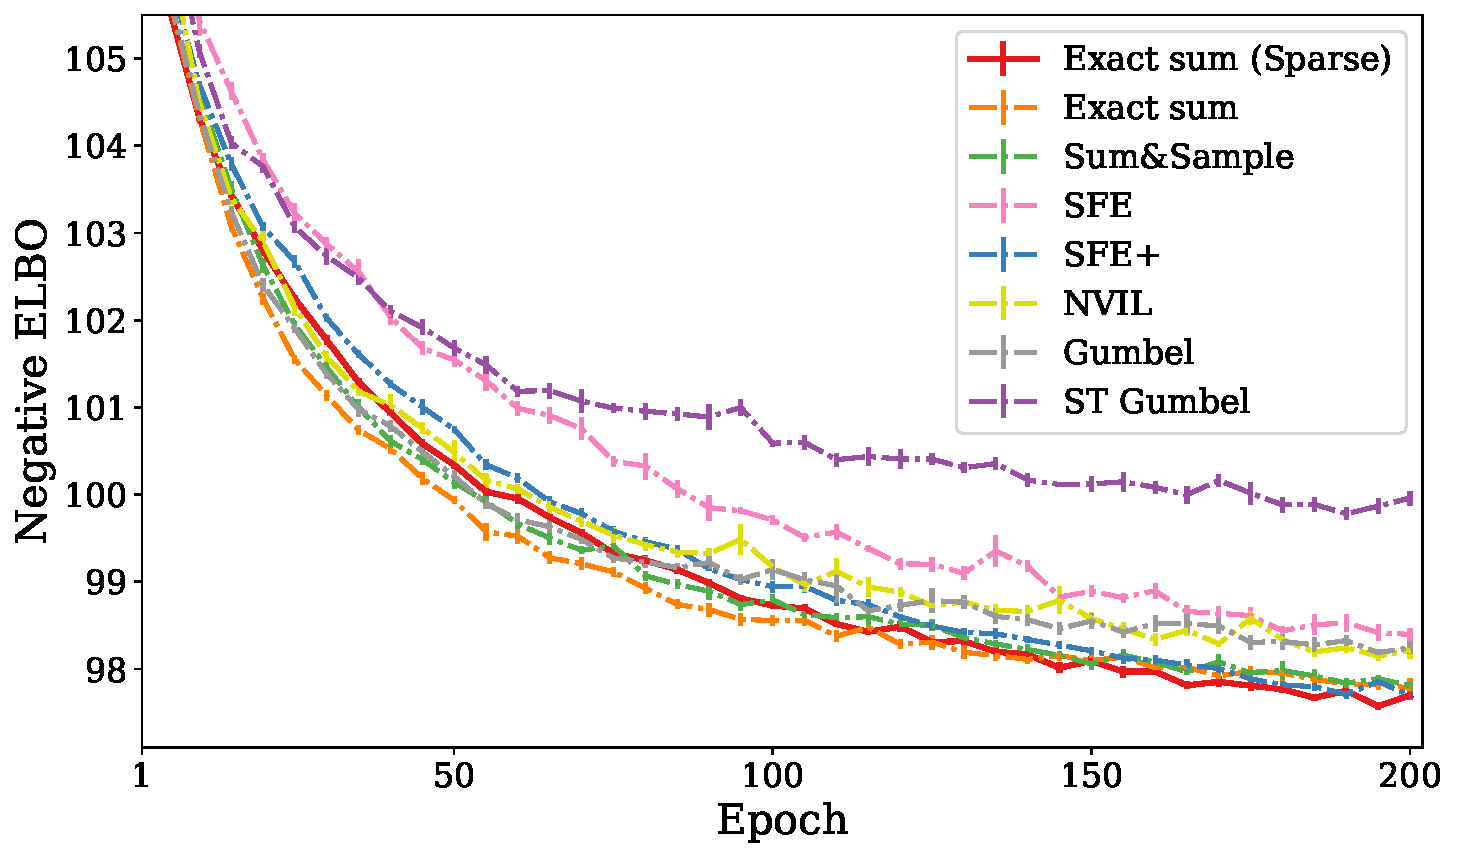
\includegraphics[width=.9\textwidth]{Figures/ss_mnist_elbo_path.pdf}
    \caption{\label{fig:ssvaeelbo}Learning curves on the test set for semi-supervised VAE on MNIST.}
\end{figure}


\begin{table}[t]
    \centering
    \tlfstyle
    \begin{tabular}{lrr}
        \toprule
        Method &
        Accuracy (\%)
               & Decoder calls                                                \\
        \midrule

        \multicolumn{3}{l}{\emph{Monte Carlo}}                                \\
        SFE
               & 94.75{\color{gray}$\pm$ .002} & 1                            \\
        SFE$+$
               & 96.53{\color{gray}$\pm$ .001} & 2                            \\
        NVIL
               & 96.01{\color{gray}$\pm$ .002} & 1                            \\
        Sum\&Sample
               & 96.73{\color{gray}$\pm$ .001} & 2                            \\
        Gumbel
               & 95.46{\color{gray}$\pm$ .001} & 1                            \\
        ST Gumbel
               & 86.35{\color{gray}$\pm$ .006} & 1                            \\
        \spacerule
        \multicolumn{3}{l}{\emph{Marginalization}}                            \\
        Dense
               & 96.93{\color{gray}$\pm$ .001} & 10                           \\
        Sparse {\small \color{gray}{(proposed)}}
               & 96.87{\color{gray}$\pm$ .001} & 1.01{\color{gray}$\pm$ 0.01} \\
        \bottomrule
    \end{tabular}
    \caption{\label{tab:ssvaeelbo}
        Average test results and standard errors over 10 runs for semi-supervised VAE on MNIST.}
\end{table}

We consider the semi-supervised Variational Auto-Encoder (VAE) of \citet{KingmaEtAl2014SSVAE},
which models the joint probability $p(z,h,x|\phi)=p(z)p(h)p(x|z,h)$, where
$x$ is an observation (an MNIST image), $h$ is a continuous latent
variable with a $n$-dimensional standard Gaussian prior, and $z$ is a
discrete random variable with a uniform prior over $K$ categories.
The marginal $p(x | \phi) = \sum_{z=1}^K \int_h p(x | z, h,
    \phi)p(h)p(z) \dd h$ is intractable, due to the marginalization of $h \in
    \mathbb R^n$. For a fixed $h$ (\eg, sampled), marginalizing $z$
requires $K$ calls to the decoder, which can be costly depending on
the decoder's architecture.

To circumvent the need for the marginal likelihood,
\citet{KingmaEtAl2014SSVAE} use variational inference
\citep{Jordan+1999:VI} with an approximate posterior $\pi(z|x,
    \theta_\pi)q(h|z,x, \lambda)$. This trains a
classifier $\pi(z|x, \theta_\pi)$ along with the generative model. In
\citet{KingmaEtAl2014SSVAE}, $h$ is sampled with a
reparameterization, and the expectation over $z$ is computed in
closed-form, that is, assessing all $K$ terms of the sum for a
sampled $h$. Under the notation in \secref{sec:lvm},
we let $\theta_\ell = \{\lambda, \phi\}$ and define
$\pi(z|x, \theta_\pi) \defeq q(z|x, \lambda)$ and
%
\begin{align}
    \begin{split}
        \ell(x, z; \theta_\ell) \defeq
        & - \mathbb E_{q(h|z,  \lambda)}\left[ \log p(x \mid z, h, \phi) \right] \\
        & - \log \frac{p(z)}{\pi(z \mid x, \theta_\pi)}                          \\
        & + \KL\left[q(h \mid x, z, \lambda) \,\,\|\,\, p(h)\right],
        \label{eq:elbonotation}
    \end{split}
\end{align}
%
which turns \eqnref{eq:fit} into the (negative) evidence lower bound
(ELBO). To update $q(h | x, z, \lambda)$, we use the
reparameterization trick to obtain gradients through a sampled $h$.
For $\pi(z | x, \theta_\pi)$, we may still explicitly marginalize over
each possible assignment of $z$, but this has a multiplicative cost
on $K$. As an alternative, we parameterize $\pi(z|x,
    \theta_\pi)$ with a sparse mapping, comparing it to the original
formulation and with stochastic gradients based on SFE and continuous
relaxations of $z$.

\paragraph*{Data and architecture.} We evaluate this model on the
MNIST dataset~\citep{lecun1998gradient}, using 10\% of labeled data,
treating the remaining data as unlabeled. MNIST consists of $28
    \times 28$ gray-scale images of hand-written digits. It contains
60,000 datapoints for training and 10,000 datapoints for testing. We
perform model selection on the last 10,000 datapoints of the training
split. In this experiment, the classification network consists of
three fully connected hidden layers of size 256, using ReLU
activations. The generative and inference network both consist of one
hidden layer of size 128, also with ReLU activations. The
multivariate Gaussian has 8 dimensions and its covariance is
diagonal. For all models we have chosen the learning rate based on
the best ELBO on the validation set, doing a grid search (5e-5, 1e-4,
5e-4, 1e-3, 5e-3). The accuracy shown in \tableref{tab:ssvaeelbo} is
the test accuracy taken after the last epoch of training. The
temperature of the Gumbel models was annealed according to $\tau =
    \max\left(0.5, -rt\right)$, where $t$ is the global training step.
For these models, we also did a grid search over $r$ (1e-5, 1e-4) and
over the frequency of updating $\tau$ every (500, 1000) steps.
Optimization was done with Adam. For our method, in the labeled loss
component of the semi-supervised objective we used the sparsemax
loss~\citep{martins2016softmax}. Following \citet{RB19}, we pretrain
the network with only labeled data prior to training with the whole
training set. Likewise, for our method, we pretrained the network on
the sparsemax loss and every other method with the Negative
Log-Likelihood loss. Each model was trained for 200 epochs.

\paragraph*{Comparisons.} Our proposal's key ingredient is sparsity,
which permits exact marginalization and a deterministic gradient. To
investigate the impact of sparsity alone, we report a comparison
against the exact marginalization over the entire support $\ZZ$ using
a dense softmax parameterization. To investigate the impact of
deterministic gradients, we compare to stochastic gradients:

\begin{itemize}
    \item SFE with a moving average baseline;
    \item SFE with a self-critic
          baseline~\citep[SFE+;][]{rennie2017self}, that is, we use $\log
              p(x|z', h, \phi)$ as baseline, where $z' \sim \pi(z|x, \theta_\pi)$
          is an independent sample;
    \item NVIL~\citep{mnih2014neural}
          with a learned baseline (we train a MLP to predict the learning
          signal by minimizing mean squared error);
          \footnote{NVIL and SFE+ are
              similar, the difference being that the baseline in SFE+ does not
              require additional parameters nor it introduces additional
              objectives.}
    \item Sum-and-sample~\citep{RB19};
    \item Gumbel-Softmax, which relaxes the random variable to the interior of the simplex;
    \item ST Gumbel-Softmax, which discretizes the relaxation in
          the forward pass, but ignores the discretization function in the
          backward pass.\footnote{For Gumbel-Softmax (with and
              without ST), we follow \citet{GumbelSoftmax} and substitute
              $\KL(\pi(z|x, \theta_\pi) \| p(z))$ in the ELBO by the $\KL$
              divergence of $\Cat(\softmax(\s))$ from a discrete uniform prior.
              Strictly speaking this means the objective is not a proper ELBO and
              its relationship to an ELBO is unclear~\citep[Appendix
                  C.2]{Concrete}.}
\end{itemize}

\paragraph*{Results and discussion.}

In \figref{fig:ssvaeelbo}, we see that our proposed sparse
marginalization approach performs just as well as its dense
counterpart, both in terms of ELBO and accuracy. However, by
inspecting the number of times each method calls the decoder for
assessments of $p(x|z, h,\phi)$, we can see that the effective
support of our method is much smaller\,---\,sparsemax-parameterized
posteriors get very confident, and mostly require one, and sometimes
two, calls to the decoder. Regarding the Monte Carlo methods, the
continuous relaxation done by Gumbel-Softmax underperformed all the
other methods, with the exception of SFE with a moving average. While
SFE+ and Sum\&Sample are very strong performers, they will always
require throughout training the same number of calls to the decoder
(in this case, two). On the other hand, sparsemax makes a small
number of decoder calls not due to a choice in hyperparameters but
thanks to the model converging to only using a small support, which
can endow this method with a lower number of computations as it
becomes more confident.

\subsection{Emergent Communication Game}\label{sec:comm}

Emergent communication studies how two agents can develop a
communication protocol to solve a task
collaboratively~\citep{kirby2002natural}. Recent work used neural
latent variable models to train these agents via a ``collaborative
game'' between
them~\citep{lewis1969convention,Lazaridou2017,Havrylov2017,
    jorge2016learning, foerster2016learning, sukhbaatar2016learning}. In
\citet{Lazaridou2017}, one of the agents (the \emph{sender}) sees an
image $v_y$ and sends a single symbol message $z$ chosen from a set
$\mathcal{Z}$ (the \emph{vocabulary}) to the other agent (the
\emph{receiver}), who needs to choose the correct image $v_y$ out of
a collection of images $\mathcal{V} = \left\{ v_1, \dots, v_C
    \right\}$.\footnote{\citet{Lazaridou2017} lets the sender see the
    full set $\mathcal{V}$. In contrast, we follow \citet{Havrylov2017}
    in showing only the correct image $v_y$ to the sender. This makes the
    game harder, as the message $z$ needs to encode a good
    ``description'' of the correct image $v_y$ instead of encoding only
    its differences from $\mathcal{V}\setminus \{v_y\}$.} They found that
the messages communicated this way can be correlated with broad
object properties amenable to interpretation by humans. In our
framework, we let $x = (\mathcal{V}, y)$ and define $\ell (x, z;
    \theta) \coloneqq -\log p(y \mid \mathcal{V}, z, \theta_\ell)$ and
$\pi (z \mid x, \theta) \coloneqq p(z \mid v_y, \theta_\pi)$, where
$p(y \mid \mathcal{V}, z, \theta_\ell)$ corresponds to the sender and
$p(z \mid v_y, \theta_\pi)$ to the receiver. Following
\citet{Lazaridou2017}, we add an entropy regularization of $\pi (z
    \mid x, \theta)$ to the loss, with a coefficient as an
hyperparameter~\citep{Mnih2016}.

\paragraph*{Data and architecture.} In this application, we closely
followed the experimental procedure described
by~\citet{Lazaridou2017} with a few key differences. The architecture
of the sender and the receiver is identical with the exception that
the sender does not take as input the distracting images along with
the correct image\,---\,only the correct image. To make the game even
harder, we increase the collection of images $|\mathcal{V}|$ as
suggested by \citet{Havrylov2017}; in our experiments, we increase it
from 2 to 16. and the vocabulary of the sender was increased to 256.
The hidden size and embedding size was also increased to 512 and 256,
respectively. We did a grid search on the learning rate (0.01, 0.005,
0.001) and entropy regularizer (0.1, 0.05, 0.01) and chose the best
configuration for each model on the validation set based on the
communication success. For the Gumbel models, we applied the same
schedule and grid search to the temperature as described in
\secref{sec:gen}. All models were trained with the Adam optimizer,
with a batch size of 64 and during 200 epochs. We choose the
vocabulary of the sender to be 256, the hidden size to be 512 and the
embedding size to be 256. All methods are trained for 500 epochs. The
data used by \citet{Lazaridou2017} is a subset of ImageNet containing
463,000 images, chosen by sampling 100 images from 463 base-level
concepts. The images are then applied a forward-pass through the
pretrained VGG ConvNet~\citep{convnet} and the representations at the
second-to-last fully connected layer are saved to use as input to the
sender/receiver.

\paragraph*{Comparisons.} We compare our method to stochastic gradient
estimators as well as exact marginalization under a dense softmax
parameterization of $p (z \mid v_y, \theta_\pi)$. Again, we have
unbiased (SFE with moving average baseline, SFE+, and NVIL) and
biased (Gumbel-Softmax and ST Gumbel-Softmax) estimators. For SFE we
also experiment using a 0/1 loss.

\begin{table}[t]
    \begin{center}
        \tlfstyle
        \begin{tabular}{lr@{~}lr}
            \toprule
            Method                                 & \multicolumn{2}{c}{Communication success (\%)} & Decoder calls                   \\
            \midrule
            {\emph{Monte Carlo}}                   &                                                &                           &     \\
            SFE (NLL)                              & 33.05                                          & {\color{gray}$\pm$ 2.84}  & 1   \\
            SFE (0/1)                              & 55.36                                          & {\color{gray}$\pm$ 2.92}  & 1   \\
            SFE$+$ (0/1)                           & 44.32                                          & {\color{gray}$\pm$ 2.72}  & 2   \\
            NVIL                                   & 37.04                                          & {\color{gray}$\pm$ 1.61}  & 1   \\
            Gumbel                                 & 23.51                                          & {\color{gray}$\pm$ 16.19} & 1   \\
            ST Gumbel                              & 27.42                                          & {\color{gray}$\pm$ 13.36} & 1   \\
            \spacerule
            \emph{Marginalization}                 &                                                &                           &     \\
            Dense                                  & 93.37                                          & {\color{gray}$\pm$ 0.42}  & 256 \\
            Sparse {\small \color{gray}(proposed)} &
            93.35                                  & {\color{gray}$\pm$ 0.50}                       &
            3.13{\color{gray}$\pm$ 0.48}                                                                                              \\
            \bottomrule
        \end{tabular}
    \end{center}
    \caption{Emergent communication success test results,
        averaged across 10 runs. Random guess baseline 6.25\%.}
    \label{tab:symbol}
\end{table}

\paragraph*{Results and discussion.}

Table~\ref{tab:symbol} shows the communication success (accuracy of
the receiver at picking the correct image $v_y$). While the
communication success for $|\mathcal{V}|=2$ in \citet{Lazaridou2017}
was close to perfect, we see that increasing $|\mathcal{V}|$ to 16
makes this game much harder to sampling-based approaches. In fact,
only the models that do explicit marginalization achieve close to
perfect communication in the test set. However, as $\ZZ$ increases,
marginalizing with a softmax parameterization gets computationally
more expensive, as it requires $|\ZZ|$ forward and backward passes on
the receiver. Unlike softmax, the model trained with sparsemax
gives a very small support, requiring on average only 3 decoder
calls. In fact, sparsemax
starts off dense while exploring, but quickly becomes very sparse
(\figref{fig:nonzero_comm}).

\begin{figure*}[ht]
    \centering
    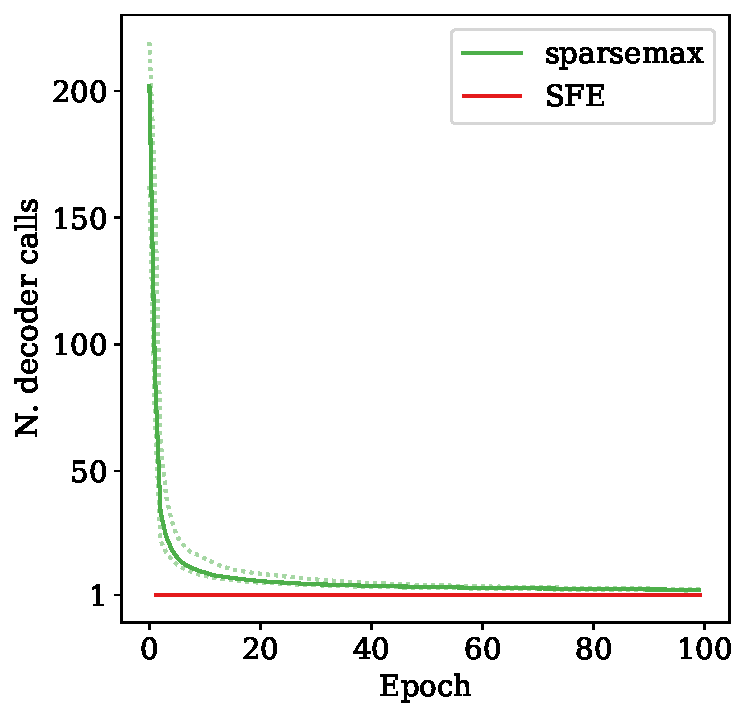
\includegraphics[width=0.65\columnwidth]{Figures/sparsemax_nonzero_em_comm.pdf}
    \caption{
        Median decoder calls per epoch during training
        time with 10 and 90 percentiles in dotted lines by sparsemax.
    }
    \label{fig:nonzero_comm}
\end{figure*}

\subsection{Bit-Vector Variational Auto-Encoder}\label{sec:bernvae}

As described in \secref{sec:structured}, in many interesting problems,
combinatorial interactions and constraints make $\ZZ$ exponentially
large. In this section, we study the illustrative case of encoding
(compressing) images into a binary codeword $z$, by training a latent
bit-vector variational autoencoder~\citep{GumbelSoftmax,
    mnih2014neural}. One approach for parameterizing the approximate
posterior is to use a Gibbs distribution, decomposable as a product
of independent Bernoulli, $q(z \mid x, \lambda) \propto
    \exp(\DP{\bm{a}_z}{\bm{t}}) = \prod_{i=1}^D q(z_i \mid x, \lambda)$,
with each $z_i$ being a Bernoulli with parameter $t_i$, and $D$ being
the number of binary latent variables. While marginalizing over all the
possible $z \in \ZZ$ is intractable, drawing samples can be done
efficiently by sampling each component independently, and the entropy
has a closed-form expression.
This efficient sampling and entropy computation relies on an independence
assumption; in general, we may not have access to such efficient
computation.

\begin{sloppypar}
    Training this VAE to minimize the negative ELBO corresponds to
    $\ell(x, z; \theta_\ell) \defeq - \log \frac{p(x, z | \phi)}{q(z | x,
            \lambda)} $; we use a uniform prior $p(z)=1/|\ZZ|=1/{2^D}$. This
    objective does not constrain $\pi(z| x,\theta_\pi) \defeq q(z \mid x,
        \lambda)$ to the Gibbs parameterization, and thus to apply our
    methods we will differ from it.
\end{sloppypar}

\paragraph*{Top-{\boldmath $k$} sparsemax parameterization.} As pointed
out in \secref{sec:structured}, we cannot explicitly handle the
structured sparsemax distribution $\pv = \sparsemax(\s)$, as it
involves a vector of dimension $2^D$. However, given $\bm{t}$, we can
efficiently find the $k$ largest configurations in time
$\mathcal{O}(kD)$, with the procedure described in
\secref{sec:topksparse}, and thus we can evaluate $\sparsemaxk(\s)$
efficiently.

\paragraph*{\smap parameterization.} Another sparse alternative to the
intractable structured sparsemax, as discussed in
\secref{sec:structured}, is \smap. In this case, we compute an optimal
distribution $\pv$ using the active set algorithm of
\citet{niculae2018sparsemap}, by using a maximization oracle which
can be computed in $\mathcal{O}(D)$:
\begin{equation}
    \argmax_z \DP{\bm{a}_z}{\bm{t}} = z^\star \quad \text{s.t.}\quad
    [\bm{a}_{z^\star}]_i = \begin{cases}
        1, & t_i \geq 0 \\
        0, & t_i < 0    \\
    \end{cases}.
\end{equation}
Since SparseMAP can handle structured problems, we also experimented
with adding a \emph{budget constraint} to SparseMAP: this is done by
adding a constraint $\|\bm{z}\|_1 \le B$, where $B \le D$; we used
$b=\frac{D}{2}$. The budget constraint ensures the images are
represented with sparse codes, and the maximization oracle can be
computed in $\mathcal{O}(D \log D)$. This
is done by sorting the Bernoulli scores and selecting the entries
among the top-$B$ which have a positive score.

We stress that, with both top-$k$ sparsemax and \smap parameterizations,
$z$ does not decompose into a product of independent
binary variables: this property is specific to the Gibbs parameterization.
However, since these new approaches induce a very sparse approximate posterior
$q$, we may compute the terms $\EE_{q(z\mid x, \lambda)} [\log p(x \mid z,
        \phi)]$ and $\EE_{q(z\mid x, \lambda)} [\log q(z \mid x, \lambda)]$
explicitly.

\begin{figure}[htbp]
    \centering
    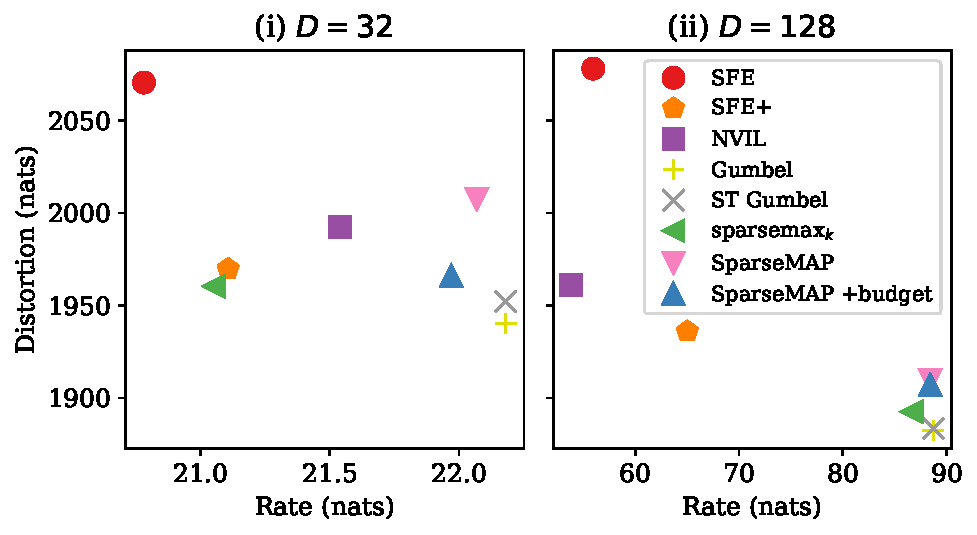
\includegraphics[width=0.95\textwidth]{Figures/distortion-rate.pdf}
    \caption{\label{fig:distortion_rd}Test results for Fashion-MNIST. RD plots
        (the closer to the lower right corner, the better).}
\end{figure}

\begin{table}
    \centering
    \tlfstyle
    \begin{tabular}{lrr}
        \toprule
        Method            & $D=32$ & $D=128$       \\
        \midrule
        \multicolumn{3}{l}{\emph{Monte Carlo}}     \\
        SFE               & 3.74   & 3.77          \\
        SFE$+$            & 3.61   & 3.59          \\
        NVIL              & 3.65   & 3.60          \\
        Gumbel            & 3.57   & 3.49          \\
        ST Gumbel         & 3.53   & 3.55          \\
        \spacerule
        \multicolumn{3}{l}{\emph{Marginalization}} \\
        Top-$k$ sparsemax & 3.62   & 3.61          \\
        \smap             & 3.72   & 3.67          \\
        \smap (w/ budget) & 3.64   & 3.66          \\
        \bottomrule
    \end{tabular}
    \vspace{5pt}
    \caption{\label{tab:distortion_tab}
        Test results for Fashion-MNIST. NLL in bits/dim (lower, the better).}
\end{table}

\paragraph*{Data and architecture.} We use
Fashion-MNIST~\citep{fmnist}, consisting of $28 \times 28$, 256-level
gray-scale images of clothes. It contains 60K datapoints for training
and 10K datapoints for testing. We perform model selection on the
last 10K datapoints of the training split. The decoder uses an
independent categorical distribution for each pixel, $p(x \mid z,
    \phi) = \prod_{i=1}^{28} \prod_{j=1}^{28} p(x_{ij} \mid z, \phi)$.
For top-$k$ sparsemax, we choose $k=10$. We have set the generative
and inference network to consist of one hidden layer with 128 nodes,
using ReLU activations. We have searched a learning rate doing grid
search (0.0005, 0.001, 0.002) and chosen the model based on the ELBO
performance on the validation set. For the Gumbel models, we applied
the same schedule and grid search to the temperature as described in
\secref{sec:gen}. We used the Adam optimizer.

\begin{sloppypar}
    \paragraph*{Comparisons.} This time, exact marginalization under a
    dense parameterization of $q (z | x, \lambda)$ is truly intractable,
    so we can only compare our method to stochastic gradient estimators.
    We have unbiased SFE-based estimators (SFE with moving average
    baseline, SFE+, and NVIL), and biased reparameterized gradient
    estimators (Gumbel-Softmax and ST Gumbel-Softmax). As there is no
    supervision for the latent code, we cannot compare the methods in
    terms of accuracy or task success. Instead, we display the trained
    models in the rate-distortion (RD)
    plane~\citep{Alemi2018}\footnote{Distortion is the expected value of
        the reconstruction negative log-likelihood, while rate is the average
        KL divergence from the prior to the approximate posterior.} and also
    report bits-per-dimension of $x$, estimated with importance sampling,
    on held-out data.
\end{sloppypar}

\begin{sloppypar}
    Bits-per-dimension is the negative logarithm of marginal likelihood
    normalized per number of pixels in the image, thus we need to assess
    or estimate the marginal likelihood of observations. For dense
    parameterizations, the usual option is importance sampling (IS) using
    the trained approximate posterior as importance distribution: \ie,
    $\log p(x|\phi) \overset{\text{IS}}{\approx} \log \left(\frac{1}{S}
        \sum_{s=1}^S \frac{p(z^{(s)}, x|\phi)}{q(z^{(s)} | x, \lambda)}
        \right)$ with $z^{(s)} \sim q(z|x, \lambda)$. The result is a
    stochastic lower bound which converges to the true log-marginal in
    the limit as $S \to \infty$. With a sparse posterior approximation we
    can split the marginalization
\end{sloppypar}

\begin{equation}
    \log p(x|\phi) = \log \left( \sum_{z \in \bar \ZZ}
    p(z)p(x|z, \phi) + \sum_{z \in \ZZ \setminus \ZZ} p(z)p(x|z, \phi)
    \right)
\end{equation}

\noindent into one part that handles outcomes in the support $\bar \ZZ$ of the
sparse posterior approximation and another that handles the
outcomes in the complement set $\ZZ \setminus \bar \ZZ$. We compute
the first part exactly and estimate the second part via rejection
sampling from $p(z)$.

\paragraph*{Results and discussion.} \tableref{tab:distortion_tab}
shows an importance sampling estimate ($1024$ samples per test
example were taken) of the negative log-likelihood for the several
methods, together with the converged values of each method in the RD
plane in \figref{fig:distortion_rd}. Both show results for which the
bit-vector has dimensionality $D=32$ and $D=128$. Regarding the
estimated negative log-likelihood, our methods exhibit increased
performance when compared to SFE, and top-$k$ sparsemax is
competitive with the remaining unbiased estimators. However, in the
RD plane, both our methods show comparable performance to SFE$+$ and
NVIL for $D=32$, but for $D=128$ all of our methods have a
significantly higher rate and lower distortion than any unbiased
estimator, suggesting a better fit of $p(x|\phi)$~\citep{Alemi2018}.
In \figref{fig:structcalls}, we can observe the training progress in
number of calls to $p(x \mid z, \phi)$ for the models with 32 and 128
latent bits, respectively. While $\sparsemaxk$ introduces bias
towards the most probable assignments and may discard outcomes that
$\sparsemax$ would assign non-zero probability to, as training
progresses distributions may (or tend to) be sufficiently sparse and
this mismatch disappears, making the gradient computation exact.

\begin{figure}[htbp]
    \centering
    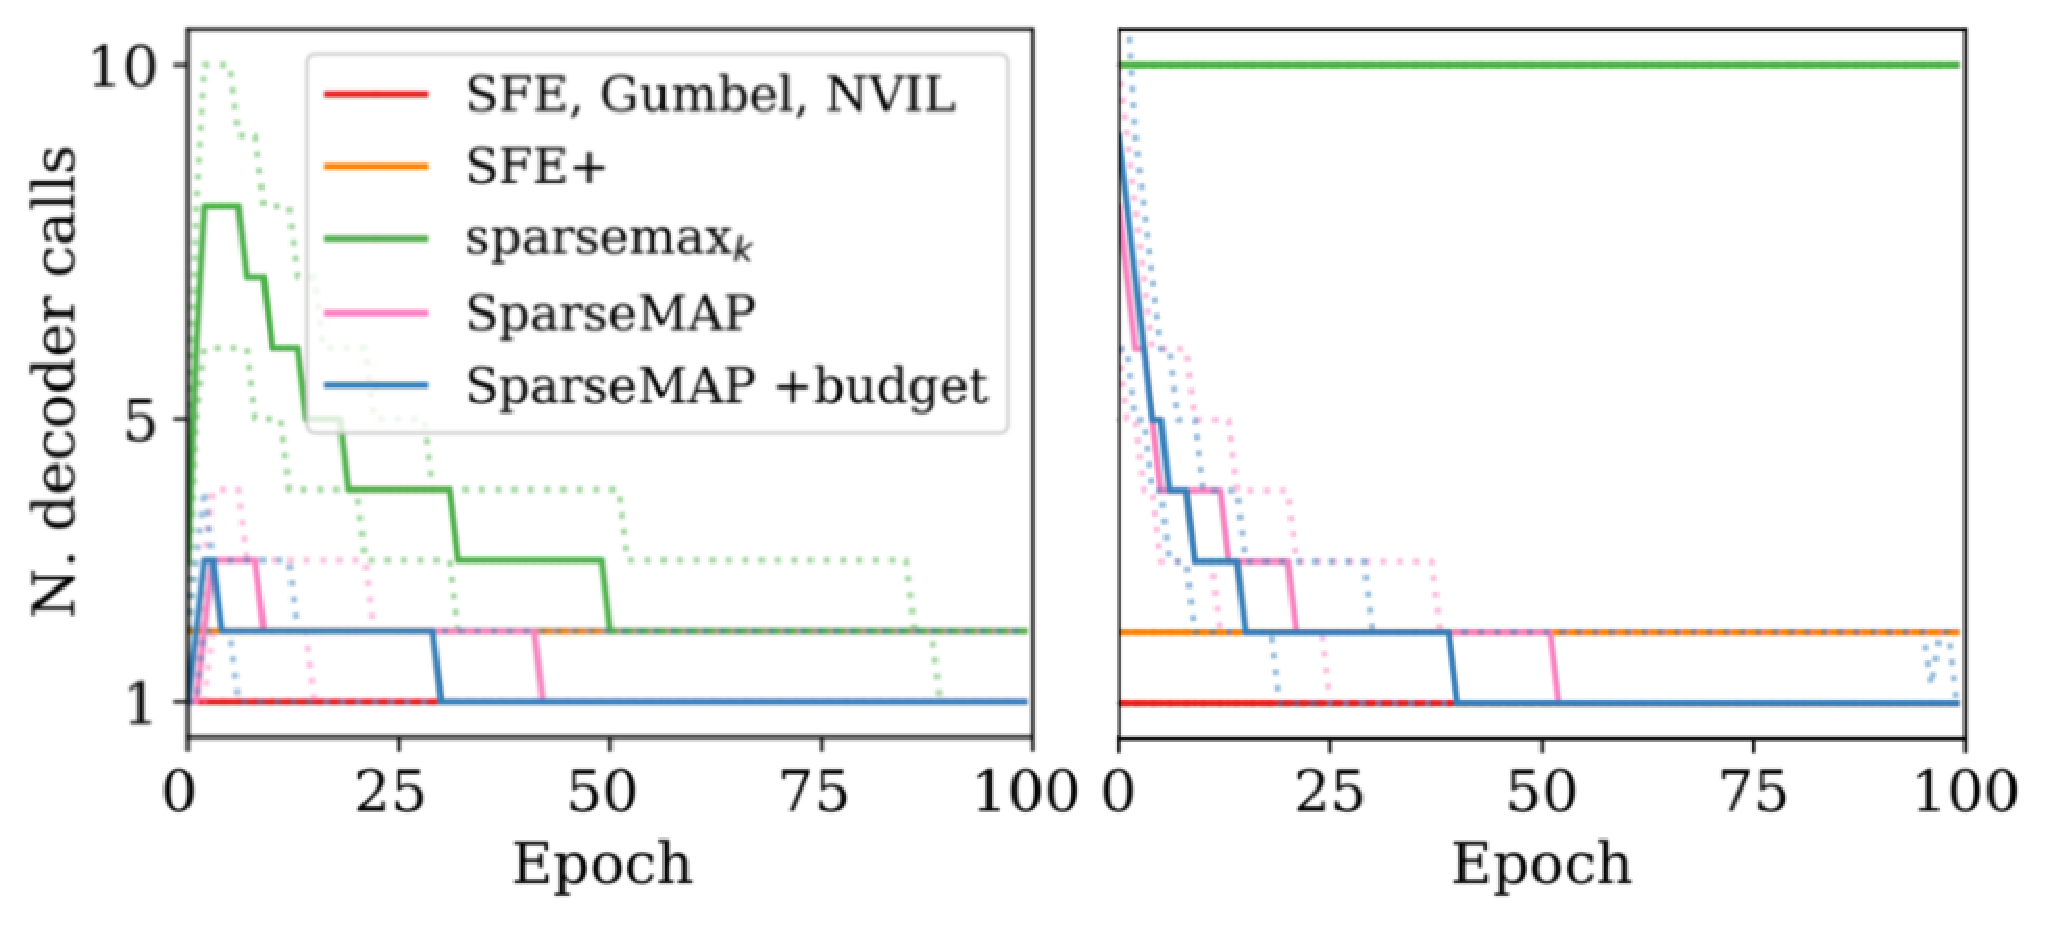
\includegraphics[width=0.95\textwidth]{Figures/spars.pdf}
    \caption{Bit vector VAE median and quartile decoder calls per
        epoch,
        $D=32$ (left) / $D=128$ (right).\label{fig:structcalls}}
\end{figure}

Remarkably, this happens for $D\!=\!32$\,---\,the support of
$\sparsemaxk$ is smaller than $k$, giving the true gradient to
$q(z\mid x, \lambda)$ for most of the training. This no longer
happens for $D\!=\!128$, for which it remains with full support
throughout, due to the much larger search space. On the other hand,
\smap solutions become very sparse from the start in both cases,
while still obtaining good performance. There is, therefore, a
trade-off between the solutions we propose: on one hand,
$\sparsemaxk$ can become exact with respect to the expectation in
\eqnref{eq:fit}, but it only does so if the chosen $k$ is suitable to
the difficulty of the model; on the other hand, \smap may not offer
an exact gradient to $q(z\mid x, \lambda)$, but its performance is
very close to $\sparsemaxk$ and its higher propensity for sparsity
gifts it with less computation. \figref{fig:elbo_bit} shows the
downstream loss (ELBO) over epochs and over the median number of
decoder calls per epoch. The plots on \figref{fig:elbo_bit_calls}
show how our methods have comparable computational overhead to
sampling approaches. Oftentimes, our methods could have been trained
in less epochs to obtain the same performance as the sampling
estimators have for 100 epochs.

\begin{figure}[ht]
    \centering
    \begin{subfigure}[b]{0.49\textwidth}
        \centering
        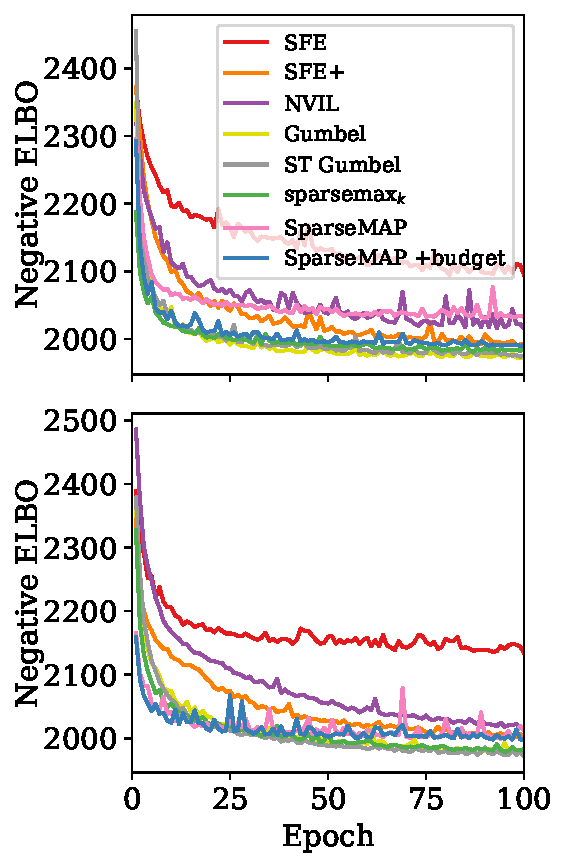
\includegraphics[width=\textwidth]{Figures/elbo-bit-vector.pdf}
        \caption{Neg. ELBO over training epochs.}
        \label{fig:elbo_bit_epochs}
    \end{subfigure}
    \begin{subfigure}[b]{0.49\textwidth}
        \centering
        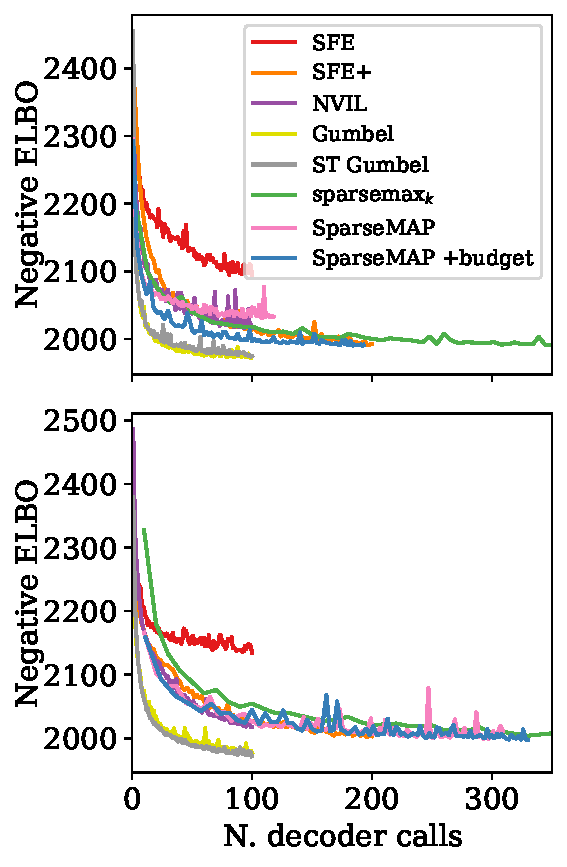
\includegraphics[width=\textwidth]{Figures/elbo-calls.pdf}
        \caption{Neg. ELBO over decoder calls.}
        \label{fig:elbo_bit_calls}
    \end{subfigure}
    \caption{Performance on the validation set
        for the experiment in \secref{sec:bernvae},
        $D=32$ (top) / $D=128$ (bottom). For $D=32$, top-$k$ sparsemax continues
        until a total of 561 median decoder calls, and for $D=128$ it continues
        until a total of 998.}
    \label{fig:elbo_bit}
\end{figure}

Concerning relaxed estimators, note that the reconstruction loss is
computed given a continuous sample, rather than a discrete one,
allowing it more flexibility to directly reduce distortion and
potentially explaining why it does well in that regard. Moreover, the
rate of the relaxed model is unknown,\footnote{Estimating it would
    require a choice of Binary Concrete prior and an estimate of the KL
    divergence from that to the Binary Concrete approximate posterior
    \citep[Appendix C.3.2]{Concrete}.} and instead we plot the rate as if
$z$ was given discrete treatment, which, although common practice,
makes comparisons to other estimators inadequate. For ST
Gumbel-Softmax the situation is different since, after training, $z$
is given discrete treatment throughout. Its success shows that,
unlike in the other tasks considered, training on biased gradients is
not too problematic.

\section{Subsequent Work}
\label{sec:subsequent}

\citet{correia2020procneurips} proved to be a relevant
contribution to the field of discrete and structured latent variable
modelling. In particular, and most closely related to our work,
\citet{chen2021EvidentialSoftmaxSparse} added another method to the
family of efficient marginalization techniques that we started in
\citet{correia2020procneurips}. They introduce a new
function called \emph{ev-softmax} that has its origins in evidential
theory and evidential sparsification~\citep{itkina2020evidential}.
The properties of this function are more similar to \emph{softmax}
than \emph{sparsemax}, while still allowing for a sparse
distribution. They show that their method is less prone to
multimodality collapse~\citep{itkina2020evidential} and show improved
results in the experiment described in \secref{sec:gen}.

In another application of sparsity for discrete latent variable
models, \citet{farinhas2022SparseCommunicationMixed} introduced a new
family of mixed discrete-continuous random variables that can be used
to train these models. Their method has its origins in the recent
field of sparse and continuous
distributions~\citep{martins2020SparseContinuousAttention}. Their
method is applied to the experiments that we described in
\secref{sec:comm} and \secref{sec:bernvae} and show promising
results. As in our case, their method also bypasses the need for
methods with high variance, as in SFE, and relaxations of the
discrete space, as in Gumbel-Softmax; however, in their case, that's
not due to explicit marginalization but rather due to the nature of
the mixed random variables that they introduce.

As we will explore further in the next chapter, we believe that the
methods we have proposed here have potential for structured
applications. In particular, due to the structured nature of
language, the explicit marginalization of the structured space can
prove valuable to NLP. For example, our method has been applied
successfully for semantic
parsing~\citep{wang2021LearningExecutionsSemantic}. In this work, the
authors use our top-$k$ sparsemax method in the E-step of an EM
algorithm. Since they do not have access to a true top-$k$, they
approximate it using beam search. When compared to the other
baselines and other methods proposed, the approach that used top-$k$
sparsemax had the best performance.

\section{Final Remarks and Chapter Summary}

We described a novel training strategy for discrete latent variable
models, eschewing the common approach based on MC gradient estimation
in favor of deterministic, exact marginalization under a sparse
distribution. Sparsity leads to a powerful \textbf{adaptive} method,
which can investigate fewer or more latent assignments $z$ depending
on the ambiguity of a training instance $x$, as well as on the stage
in training. We showcase the performance and flexibility of our
method by investigating a variety of applications, with both discrete
and structured latent variables, with positive results. Our models
very quickly approach a small number of latent assignment evaluations
per sample, but make progress much faster and overall lead to
superior results.

Our proposed method thus offer the accuracy and robustness of exact
marginalization while meeting the efficiency and flexibility of score
function estimator methods, providing a promising alternative to
successfully train more \textbf{compact} neural models. As we are
learning from subsequent works (\secref{sec:subsequent}), we believe
that our method can be used to address the challenges of training
these sorts of models in a variety of applications, particularly NLP.

\cleardoublepage

\singlespacing
\fancychapter[Conclusions]{Conclusions}
\label{chap:conclusions}

\cleardoublepage
\doublespacing

\noindent To wrap up the present thesis, we review the main contributions
developed in this work, and discuss their impact, limitations, and
potential directions for future work.

\section{Summary of Contributions}

\noindent Throughout this thesis, we have developed models and
techniques that aim to make neural models more data-efficient, transparent,
and compact.

In \chapref{chap:ape}, we achieved \textbf{data-efficiency} by
leveraging the \textbf{transfer learning} power of a pre-trained
language model to avoid the need for producing a large synthetic
dataset, in the context of a real-world application: Automatic
Post-Editing.

In \chapref{chap:adaptsparse}, we proposed a model with increased
\textbf{transparency} by letting it \textbf{learn its own sparsity}.
The chosen application was NMT, and we showed
how the sparsity can help to interpret the various roles of each
attention head in the model.

Finally, in \chapref{chap:sparsemarg}, we once again leveraged
\textbf{learnable sparsity} by introducing a new method to train
latent variable models with discrete or structured nodes. We show the
efficacy of our method in several applications: semi-supervised
learning, emergent communication, and unsupervised learning of
bit-vector representations. This method achieves better performance
than standard methodologies for training discrete latent variable
models and as such aids in the development of more \textbf{compact}
neural models.

A common theme in this thesis is sparsity, particularly
sparse probability distributions. We have followed in the footsteps
of work started by \citet{sparsemax} and proposed novel uses of
these sparse distributions and promising alternatives to them.
In all works described, we have shown how in different applications
we can let neural models learn how much sparsity they need; be it
in the context of an attention mechanism, or in the context of
the number of relevant latent assignments during training.

On another front, we tackle some forms of \textbf{weak supervision}.
On one hand, we use transfer learning and minimize the amount of data
required to train an APE model in \chapref{chap:ape}. On the other
hand, we also applied our method of \chapref{chap:sparsemarg} to
obtain improved performance on a semi-supervised learning task.
Additionally, in \secref{sec:subsequent_work_adapt} we saw how our
discovered attention head roles can be used to fix attention patterns
in a Transformer, increasing inductive bias in the
process~\citep{raganato2020FixedEncoderSelfAttentiona}.

\section{Open Problems and Limitations}

\noindent In the pursuit of diligent research, we briefly discuss some of the
open problems and limitations of the work presented in this thesis.
We seek not to diminish any of these limitations, but rather present
them fairly.
We will also discuss the ethical ramifications of our
work in a later section (\secref{sec:impact}).

As previously stated, sparsity is a prominent theme in this work.
That sparsity is achieved through probability normalization functions
such as sparsemax, $\alpha$-\entmaxtext, and SparseMAP. While
sparsity can lead to increased efficiency, we do not fully take
advantage of this in the present thesis or in the publicly released
code. For example, for $\alpha$-\entmaxtext, further speed-ups are
possible, with careful engineering, by leveraging more parallelism in
the bisection algorithm for computing it.
This is a relevant research direction, as it is now possible to
exploit recent generations of GPU architectures which are more
sparse-friendly than before.

In \chapref{chap:ape}, we have used a large pre-trained model to
circumvent the need to train MT models to produce a large synthetic
dataset and then train an APE model on it. Although we believe
this to be a way to spare resources, we do not wish to underplay
the resources used to train the pre-trained model itself.

While we have shown promising results in \chapref{chap:sparsemarg},
we are aware that the experiments we conducted were performed on toy
datasets. While this may overemphasize the success of the work, we
have seen in \secref{sec:subsequent} that our method has already been
successfully applied to applications that have real-world datasets.
We hope to continue seeing this trend in the future.

\section{Future Directions}

\noindent We further list in this section exciting directions for future work
that draw inspiration from the methods proposed in this thesis. We
hope this might inspire other researchers in the field to explore
these directions and extend the ideas presented.

\paragraph*{Semi-supervised Learning.} Some forms of weak
supervision were explored in this work. In particular, we have shown
promising results in \chapref{chap:sparsemarg} by introducing a new
method to train discrete latent variable models, which can be used to
train semi-supervised models (\secref{sec:gen}). We believe that our
method can be used in real-world applications where supervision is
limited and that it will lead to better results than standard
methods. For example, in NLP, there are many applications where a
relaxation of the discrete space is not possible~\citep{Lee2019}.
We can consider the semi-supervised loss
%
\begin{equation}
    \mathcal{L}_{x}(\theta) =
    \sum_{z \in \mathcal{Z}} \pi(z | x) \ell(x, z; \theta)
    + \sum_{z \in \mathcal{Z}} \pi(z | x, y) \ell(x, y, z; \theta)
    + \mathcal{R}(\theta)\,,
\end{equation}
%
which is very similar to the loss used in \secref{sec:gen},
and apply it to more challenging datasets.
Whereas before we could only rely on high variance methods if we wished to
train such a model, we can now circumvent this limitation
by using our training method and computing deterministic gradients.

\paragraph*{Non-differentiability of the LVM learning signal.} We
note how, in \eqnref{eq:fit}, the training of the parameters that
learn $\pi(z|x;\theta)$ is decoupled from the training of the
parameters of the generative model of the downstream loss: when
marginalizing the latent variables, the downstream loss only scales
the gradients computed from $\pi(z|x;\theta)$. This means that our
method can still be applied when the downstream loss component does
not have any trainable parameters. Furthermore, that component in
\eqnref{eq:fit} can be replaced by any function, even
non-differentiable, akin to a reward signal. One example of a
real-world application where the downstream loss doesn't have
learnable parameters is the prompting of large pre-trained language
models~\citep{liu2021PretrainPromptPredict}. In this line of work,
the pre-trained model is assumed to already have the knowledge
required to handle the task at hand stored in its parameters and only
a prompt is required to generate the desired output. This problem
could be framed as a latent variable model and one could interpret a
natural language prompt as a discrete latent variable. Using the
property we just described, the downstream task can be optimized via
any differentiable or non-differentiable reward signal
%
\begin{equation}
    \mathcal{L}_{x}(\theta) =
    - \sum_{z \in \mathcal{Z}} \pi(z | x) r(x, z),
\end{equation}
%
where note that $r$ does not depend on the model's parameters $\theta$.

\paragraph*{Latent draft translation.} Related to the overall present
thesis topics of increasing transparency and compactness of neural
models in NLP, we highlight the potential of prototype
editing~\citep{guu2018GeneratingSentencesEditing,
    he2020LearningSparsePrototypes}. In this generative model, the
generative process has two main steps: (1) selecting a prototype
sequence of tokens $\bm{t}$ from a list of possible prototypes (\eg
the training data), and (2) editing that prototype by sampling a latent
edit vector $z$ that encodes the type of edit (\eg active to passive,
reordering, \textit{inter alia}). We note the promising possibility
of using this approach to NMT: While \citep{he2020LearningSparsePrototypes} apply their
sparse neural editor to language modeling, we will model instead a
conditional distribution over $\mathcal{X} \times \mathcal{Y}$:
%
\begin{equation}
    p(y, \bm{t}, \bm{z} | \bm{x}) =
    p(\bm{t} | \bm{x}; \theta)
    p(\bm{z} | \bm{x}; \theta)
    p(\bm{y} | \bm{t}, \bm{z}; \theta)\,.
\end{equation}
%
We may think of t as being a template for y\,---\,it can be a
lexicalized rule with gaps or variables, a phrase-based mapping
from a section of $\bm x$ to a string in the target language, among others.
Once again, for deterministic gradients and greater training stability, we
may use the training method proposed in \chapref{chap:sparsemarg}.

\section{Broader Impact}\label{sec:impact}

\noindent We discuss here the broader impact of our work.

First of all, we note that all of our code has been
open-sourced to ensure it's scrutinizable by
anyone and to boost any related future work that other researchers
might want to pursue.

A common theme in this thesis is transparency.
The main objective of improving such property in neural models
is to have superior explanatory power and therefore to aid in understanding cases
in which the model failed the downstream task. Interpretability of
deep neural models can be essential to better discover any ethically
harmful biases that exist in the data or in the model itself.

On the other hand, the models discussed in this work may
also pave the way for malicious use cases, such as is the case for generative models with
\emph{Deepfakes}, fake human avatars used by malevolent Twitter
users, or generation models that automatically generate fraudulent news,
often based on the large pre-trained language models used in this thesis.
Particularly, generative models as the ones used in \chapref{chap:sparsemarg}
are remarkable at sampling new instances of fake data and, with the
power of latent variables, the interpretability discussed before can
be used maliciously to further push harmful biases instead of
removing them. Furthermore, our work in \chapref{chap:sparsemarg} is promising in improving the
performance of latent variable models with several discrete
variables, that can be trained as attributes to control the sample
generation. Attributes that can be activated or deactivated at will
to generate fake data can both help beneficial and malignant users to
finely control the generated sample. Our work may be currently
agnostic to this, but we recognize the dangers and encourage effort to
combating any malicious applications.

Energy-wise, our data-efficient and compact models aim to require
less data and computation than other models that rely on a massive
amount of data and infrastructure. This makes our models ideal for
situations where data is scarce, or where there are few computational
resources to train large models. We believe that data efficiency and
compactness are a step forward in the direction of alleviating
environmental concerns of deep learning
research~\citep{strubell2019energy}. However, we note that, for
example, the adaptive sparsity of the models proposed in
\chapref{chap:sparsemarg} tend to use more resources earlier on
than standard methods. Even though in the applications shown
they consume much less as training progresses, it's not clear if that
trend is still observed in all potential applications.

Regarding sparsity, we note how sparsity may exhibit a larger risk of
disregarding certain correlations or groups of observations,
and thus may contribute to misinforming a practitioner.
Where such a model that uses sparsity informs decision-makers on matters that affect
lives, these decisions may be based on an incomplete view of the
correlations in the data and/or these correlations may be exaggerated
in harmful ways.
At this point, it is
unclear to which extent this happens and, if it does, whether it is
consistent across various uses. We believe that a better understanding
of the impact of sparsity in potentially oversimplifying correlations is an
additional interesting avenue of future work.


\cleardoublepage

\singlespacing
% \input{99.Conclusions/conclusions.tex}
\cleardoublepage
\phantomsection
\addcontentsline{toc}{chapter}{Bibliography}
%% Use with Cite and Natbib
%% check styles in https://en.wikibooks.org/wiki/LaTeX/Bibliography_Management
\bibliography{refs}
\bibliographystyle{unsrtnat}
%% Use with Biblatex (.bib file is set in Packages) (Not working)
%\printbibliography

\cleardoublepage

\begin{appendices}
    \begin{appendix}
        \pagenumbering{bychapter}
        \def\RR{{\mathbb{R}}}
\def\EE{{\mathbb{E}}}
\def\RRY{\RR^{|\cY|}}
\def\y{\bm{y}}
\def\triangleY{\triangle^{|\cY|}}
\def\sizeY{{|\cY|}}
\def\cC{{\mathcal{C}}}
\def\cD{{\mathcal{D}}}
\def\cX{{\mathcal{X}}}
\def\cY{{\mathcal{Y}}}

\fancychapter{Proof of Proposition~\ref{prop:grad_alpha}}\label{app:fenchelyoung}

\cleardoublepage
\onehalfspacing

\section*{Jacobian of {\boldmath $\alpha$}-\entmaxtext \wrt the shape parameter
      {\boldmath $\alpha$}}
\label{app:alpha_grad}

Recall that the \entmaxtext transformation is defined as:
\begin{equation}\label{eq:entmax_form_supp}
    \aentmax(\bm{z}) \coloneqq
    \argmax_{\p \in \simplex^d} \bm{p}^\top\bm{z} + \HHt_{\alpha}(\bm{p}),
\end{equation}
where $\alpha \geq 1$ and $\HHt_{\alpha}$ is the Tsallis entropy,
\begin{equation}%
    \HHt_{\alpha}(\bm{p})\!\coloneqq\!
    %(\alpha-1)^{-1} \left(1 - \sum_j p_j^{\alpha}\right)
    %= k(\alpha-1)^{-1}(1 - \|\p\|_{\alpha}^{\alpha}
    \begin{cases}
        \frac{1}{\alpha(\alpha-1)}\sum_j\!\left(p_j - p_j^\alpha\right)\!, &
        \!\!\!\alpha \ne 1,                                                  \\
        \HHs(\bm{p}),                                                      &
        \!\!\!\alpha = 1,
    \end{cases}
\end{equation}
and $\HHs(\bm{p}):= -\sum_j p_j \log p_j$ is the Shannon entropy.

In this section, we derive the Jacobian of $\entmax$ with respect to the scalar parameter $\alpha$.

\section*{General case of {\boldmath $\alpha>1$}}

From the KKT conditions associated with the optimization problem in
Eq.~\ref{eq:entmax_form_supp}, we have that the solution $\bm{p}^{\star}$ has the following form, coordinate-wise:
\begin{equation}\label{eq:p_kkt}
    p_i^{\star} = [(\alpha-1)(z_i - \tau^{\star})]_+^{1/(\alpha-1)},
\end{equation}
where $\tau^{\star}$ is a scalar Lagrange multiplier that ensures that
$\bm{p}^{\star}$ normalizes to 1, \ie, it is defined implicitly by the condition:
\begin{equation}\label{eq:tau_condition}
    \sum_i [(\alpha-1)(z_i - \tau^{\star})]_+^{1/(\alpha-1)} = 1.
\end{equation}
For general values of $\alpha$, Eq.~\ref{eq:tau_condition} lacks a closed form solution. This makes the computation of the
Jacobian
\begin{equation}
    \frac{\partial \aentmax(\bm{z})}{\partial \alpha}
\end{equation}
non-trivial. Fortunately, we can use the technique of implicit differentiation
to obtain this Jacobian.

The Jacobian exists almost everywhere, and the expressions we derive
expressions yield a generalized Jacobian~\citep{clarke_book} at any
non-differentiable points that may occur for certain ($\alpha$, $\x$)
pairs. We begin by noting that $\frac{\partial p_i^{\star}}{\partial
    \alpha} = 0$ if $p_i^{\star} = 0$, because increasing $\alpha$ keeps
sparse coordinates sparse.\footnote{This follows from the margin
    property of $\HHt_\alpha$~\citep{blondel2019learning}.}
Therefore we need to worry only
about coordinates that are in the support of $\bm{p}^\star$. We will assume
hereafter that the $i$\textsuperscript{th} coordinate of $\bm{p}^\star$ is non-zero.
We have:
\begin{eqnarray}\label{eq:gradient_alpha_01}
    \frac{\partial p_i^{\star}}{\partial \alpha} &=& \frac{\partial}{\partial \alpha} [(\alpha-1)(z_i - \tau^{\star})]^{\frac{1}{\alpha-1}}\nonumber\\
    &=& \frac{\partial}{\partial \alpha} \exp \left[\frac{1}{\alpha-1} \log [(\alpha-1)(z_i - \tau^{\star})]\right]\nonumber\\
    &=& p_i^{\star} \frac{\partial}{\partial \alpha} \left[\frac{1}{\alpha-1} \log [(\alpha-1)(z_i - \tau^{\star})]\right]\nonumber\\
    &=& \frac{p_i^{\star}}{(\alpha-1)^2} \left[\frac{\frac{\partial}{\partial \alpha} [(\alpha-1)(z_i - \tau^{\star})]}{z_i - \tau^{\star}} - \log[(\alpha-1)(z_i - \tau^{\star})] \right]\nonumber\\
    &=& \frac{p_i^{\star}}{(\alpha-1)^2} \left[\frac{z_i - \tau^{\star} - (\alpha-1)\frac{\partial \tau^{\star}}{\partial \alpha} }{z_i - \tau^{\star}} - \log[(\alpha-1)(z_i - \tau^{\star})] \right]\nonumber\\
    &=& \frac{p_i^{\star}}{(\alpha-1)^2} \left[1 - \frac{\alpha-1}{z_i - \tau^{\star}}\frac{\partial \tau^{\star}}{\partial \alpha} - \log[(\alpha-1)(z_i - \tau^{\star})] \right].
\end{eqnarray}
We can see that this Jacobian depends on $\frac{\partial \tau^{\star}}{\partial \alpha}$, which we now compute using implicit differentiation.

Let $\mathcal{S} = \{i: \pp^\star_i > 0 \}$).
By differentiating both sides of Eq.~\ref{eq:tau_condition}, re-using some of
the steps in Eq.~\ref{eq:gradient_alpha_01}, and recalling Eq.~\ref{eq:p_kkt},
we get
\begin{eqnarray}\label{eq:gradient_tau_implicit}
    0 &=& \sum_{i \in \mathcal{S}} \frac{\partial}{\partial \alpha} [(\alpha-1)(z_i - \tau^{\star})]^{1/(\alpha-1)}\nonumber\\
    &=& \sum_{i \in \mathcal{S}} \frac{p_i^{\star}}{(\alpha-1)^2} \left[1 - \frac{\alpha-1}{z_i - \tau^{\star}}\frac{\partial \tau^{\star}}{\partial \alpha} - \log[(\alpha-1)(z_i - \tau^{\star})] \right]\nonumber\\
    &=&  \frac{1}{(\alpha-1)^2} - \frac{\partial \tau^{\star}}{\partial \alpha} \sum_{i \in \mathcal{S}} \frac{p_i^{\star}}{(\alpha - 1)(z_i - \tau^{\star})} - \sum_{i \in \mathcal{S}} \frac{p_i^{\star}}{(\alpha-1)^2} \log[(\alpha-1)(z_i - \tau^{\star})] \nonumber\\
    &=&  \frac{1}{(\alpha-1)^2} - \frac{\partial \tau^{\star}}{\partial \alpha} \sum_{i} (p_i^{\star})^{2-\alpha} - \sum_{i} \frac{p_i^{\star}}{\alpha-1} \log p_i^{\star}\nonumber\\
    &=&  \frac{1}{(\alpha-1)^2} - \frac{\partial \tau^{\star}}{\partial \alpha} \sum_{i} (p_i^{\star})^{2-\alpha} + \frac{\HHs(\bm{p}^*)}{\alpha-1},
\end{eqnarray}
from which we obtain:
\begin{eqnarray}\label{eq:gradient_tau}
    \frac{\partial \tau^{\star}}{\partial \alpha} &=& \frac{\frac{1}{(\alpha-1)^2} + \frac{\HHs(\bm{p}^{\star})}{\alpha-1}}{\sum_i (p_i^{\star})^{2-\alpha}}.
\end{eqnarray}

Finally, plugging Eq.~\ref{eq:gradient_tau} into Eq.~\ref{eq:gradient_alpha_01}, we get:
\begin{eqnarray}\label{eq:gradient_alpha}
    \frac{\partial p_i^{\star}}{\partial \alpha} &=&  \frac{p_i^{\star}}{(\alpha-1)^2} \left[1 - \frac{1}{(p_i^{\star})^{\alpha-1}}\frac{\partial \tau^{\star}}{\partial \alpha} - (\alpha-1)\log p_i^{\star} \right]\nonumber\\
    &=&  \frac{p_i^{\star}}{(\alpha-1)^2} \left[1 - \frac{1}{(p_i^{\star})^{\alpha-1}}\frac{\frac{1}{(\alpha-1)^2} + \frac{\HHs(\bm{p}^{\star})}{\alpha-1}}{\sum_i (p_i^{\star})^{2-\alpha}} - (\alpha-1)\log p_i^{\star} \right]\nonumber\\
    &=& \frac{p_i^{\star} - \tilde{p}_i(\alpha)}{(\alpha-1)^2} - \frac{p_i^{\star}\log p_i^{\star} + \tilde{p}_i(\alpha)\HHs(\bm{p}^{\star})}{\alpha-1},
\end{eqnarray}
where we denote by
\begin{equation}
    \tilde{p}_i(\alpha) = \frac{(p_i^{\star})^{2-\alpha}}{\sum_j (p_j^{\star})^{2-\alpha}}.
\end{equation}
The distribution $\tilde{\bm{p}}(\alpha)$ can be interpreted as a ``skewed''
distribution obtained from $\bm{p}^{\star}$, which appears in the Jacobian of
$\aentmax(\x)$ \wrt $\x$ as well~\cite{entmax}.


\section*{Solving the indetermination for {\boldmath $\alpha=1$}}

We can write Eq.~\ref{eq:gradient_alpha} as
\begin{eqnarray}\label{eq:gradient_alpha_fraction}
    \frac{\partial p_i^{\star}}{\partial \alpha} &=&
    \frac{p_i^{\star} - \tilde{p}_i(\alpha) - (\alpha-1)(p_i^{\star}\log p_i^{\star} + \tilde{p}_i(\alpha)\HHs(\bm{p}^{\star}))}{(\alpha-1)^2}.
\end{eqnarray}
When $\alpha \rightarrow 1^+$, we have $\tilde{\bm{p}}(\alpha) \rightarrow \bm{p}^{\star}$, which leads to a $\frac{0}{0}$ indetermination.

To solve this indetermination, we will need to apply L'H\^opital's rule twice.
Let us first compute the derivative of $\tilde{p}_i(\alpha)$ with respect to $\alpha$. We have
\begin{equation}
    \frac{\partial}{\partial \alpha} (p_i^\star)^{2-\alpha} = -(p_i^{\star})^{2-\alpha} \log p_i^{\star},
\end{equation}
therefore
\begin{eqnarray}
    \frac{\partial}{\partial \alpha} \tilde{p}_i(\alpha) &=& \frac{\partial}{\partial \alpha} \frac{(p_i^\star)^{2-\alpha}}{\sum_j (p_j^\star)^{2-\alpha}}\nonumber\\
    &=& \frac{-(p_i^{\star})^{2-\alpha} \log p_i^{\star} \sum_j (p_j^\star)^{2-\alpha} + (p_i^{\star})^{2-\alpha} \sum_j (p_j^{\star})^{2-\alpha} \log p_j^{\star}}{\left( \sum_j (p_j^\star)^{2-\alpha} \right)^2}\nonumber\\
    &=& -\tilde{p}_i(\alpha)\log p_i^{\star} + \tilde{p}_i(\alpha) \sum_j \tilde{p}_j(\alpha) \log p_j^{\star}.
\end{eqnarray}
Differentiating the numerator and denominator in Eq.~\ref{eq:gradient_alpha_fraction}, we get:
\begin{eqnarray}\label{eq:gradient_alpha_shannon_01}
    \frac{\partial p_i^{\star}}{\partial \alpha} &=&
    \lim_{\alpha \rightarrow 1^+} \frac{(1 + (\alpha-1)\HHs(\bm{p}^{\star})) \tilde{p}_i(\alpha) (\log p_i^{\star} - \sum_j \tilde{p}_j(\alpha) \log p_j^{\star}) - p_i^{\star}\log p_i^{\star} - \tilde{p}_i(\alpha) \HHs(\bm{p}^{\star})}{2(\alpha-1)} \nonumber\\
    &=& A + B,
\end{eqnarray}
with
\begin{eqnarray}\label{eq:A_shannon}
    A &=& \lim_{\alpha \rightarrow 1^+} \frac{\HHs(\bm{p}^{\star}) \tilde{p}_i(\alpha) (\log p_i^{\star} - \sum_j \tilde{p}_j(\alpha) \log p_j^{\star}) \HHs(\bm{p}^{\star})}{2}\nonumber\\
    &=& \frac{\HHs(\bm{p}^{\star}) p_i^{\star}\log p_i^{\star} + p_i^{\star} (\HHs(\bm{p}^{\star}))^2}{2},
\end{eqnarray}
and
\begin{equation}\label{eq:B_shannon}
    B = \lim_{\alpha \rightarrow 1^+} \frac{\tilde{p}_i(\alpha) (\log p_i^{\star} - \sum_j \tilde{p}_j(\alpha) \log p_j^{\star}) - p_i^{\star}\log p_i^{\star} - \tilde{p}_i(\alpha) \HHs(\bm{p}^{\star})}{2(\alpha-1)}.
\end{equation}
When $\alpha\rightarrow 1^+$, $B$ becomes again a $\frac{0}{0}$ indetermination, which we can solve by applying again L'H\^opital's rule. Differentiating the numerator and denominator in Eq.~\ref{eq:B_shannon}:
\begin{eqnarray}\label{eq:B_shannon_02}
    B &=& \frac{1}{2}\lim_{\alpha \rightarrow 1^+} \left\{ \tilde{p}_i(\alpha) \log p_i^{\star} \left(\sum_j \tilde{p}_j(\alpha) \log p_j^{\star} - \log p_i^{\star}\right) \right. \nonumber\\
    && - \tilde{p}_i(\alpha) \left(\sum_j \tilde{p}_j(\alpha) \log p_j^{\star} - \log p_i^{\star}\right) \left(\sum_j \tilde{p}_j(\alpha) \log p_j^{\star} + \HHs(\bm{p}^{\star})\right) \nonumber\\
    && \left. - \tilde{p}_i(\alpha) \sum_j \tilde{p}_j(\alpha) \log p_j^{\star} \left(\sum_k \tilde{p}_k(\alpha) \log p_k^{\star} - \log p_j^{\star}\right)\right\}\nonumber\\
    &=& \frac{-p_i^{\star} \log p_i^{\star}(\HHs(\bm{p}^{\star}) + \log p_i^{\star})
    +p_i^{\star} \sum_j p_j^{\star} \log p_j^{\star}(\HHs(\bm{p}^{\star}) + \log p_j^{\star})}{2}\nonumber\\
    &=& \frac{-\HHs(\bm{p}^{\star}) p_i^{\star}\log p_i^{\star} - p_i^{\star} (\HHs(\bm{p}^{\star}))^2 - p_i^{\star}\log^2 p_i^{\star} + p_i^{\star} \sum_j p_j^{\star}\log^2 p_j^{\star}}{2}.
\end{eqnarray}
Finally, summing Eq.~\ref{eq:A_shannon} and Eq.~\ref{eq:B_shannon_02}, we get
\begin{eqnarray}\label{eq:gradient_alpha_shannon_02}
    \frac{\partial p_i^{\star}}{\partial \alpha}\bigg|_{\alpha=1} &=& \frac{- p_i^{\star}\log^2 p_i^{\star} + p_i^{\star} \sum_j p_j^{\star}\log^2 p_j^{\star}}{2}.
\end{eqnarray}

\section*{Summary}

To sum up, we have the following expression for the Jacobian of $\aentmax$ with respect to $\alpha$:

\begin{equation}\label{eq:final_gradient_alpha_supp}
    \frac{\partial p_i^{\star}}{\partial \alpha} =
    \left\{
    \begin{array}{ll}
        \frac{p_i^{\star} - \tilde{p}_i(\alpha)}{(\alpha-1)^2} - \frac{p_i^{\star}\log p_i^{\star} + \tilde{p}_i(\alpha)\HHs(\bm{p}^{\star})}{\alpha-1}, & \text{for $\alpha > 1$}  \\
        \frac{- p_i^{\star}\log^2 p_i^{\star} + p_i^{\star} \sum_j p_j^{\star}\log^2 p_j^{\star}}{2},                                                    & \text{for $\alpha = 1$.}
    \end{array}
    \right.
\end{equation}

\cleardoublepage
\singlespacing
        \cleardoublepage
    \end{appendix}
\end{appendices}

\end{document}